% !TeX program = lualatex
% Für echtes Arial/Calibri: lualatex/xelatex + biber verwenden.
% Fallback mit pdflatex funktioniert (sans: TeX Gyre Heros).

\documentclass[11pt,a4paper]{article}

% ---------- Pakete: Sprache, Schrift, Mikrotypografie ----------
\usepackage[a4paper,margin=2cm]{geometry} % 2,00 cm Ränder
\usepackage[ngerman,english]{babel}       % Silbentrennung DE/EN
\usepackage{microtype}                    % Mikrotypografie (Silbentrennung/Zeilenumbrüche)
\usepackage[T1]{fontenc}
\usepackage[utf8]{inputenc}
\usepackage{iftex}
\ifPDFTeX
% Fallback: pdfLaTeX (Arial-ähnlich)
\usepackage[scale=0.95]{tgheros}   % TeX Gyre Heros ~ Helvetica/Arial
\renewcommand{\familydefault}{\sfdefault}
\else
% Echte Systemschriften mit Lua/XeLaTeX:
\usepackage{fontspec}
\usepackage{xcolor}
\setmainfont{Arial}[
Ligatures=TeX,
Scale=1.0
]
% Optionaler alternativer Sans-Font:
% \setmainfont{Calibri}[Ligatures=TeX,Scale=1.0]
\fi

% ---------- Zeilen & Absätze ----------
\usepackage{setspace}
\onehalfspacing                           % 1,5-zeilig
\setlength{\parindent}{0pt}               % kein Einzug
\setlength{\parskip}{6pt}                 % 6 pt Abstand nach Absatz

% ---------- Mathe, Grafik, Tabellen ----------
\usepackage{amsmath,amssymb}
\usepackage{graphicx}
\usepackage{booktabs}
\usepackage{float}
\usepackage{subcaption}
\usepackage{siunitx}
\sisetup{detect-all}                      % Sans-Serif in siunitx
\usepackage{csquotes}                     % saubere Anführungszeichen / Blockzitate
\usepackage{mwe}                          % Beispielbilder (example-image*)

% ---------- Code ----------
\usepackage{listings}

% dezente Farben
\definecolor{lwbg}{rgb}{0.98,0.98,0.98}     % leichter Hintergrund
\definecolor{lwkeyword}{rgb}{0.0,0.45,0.30} % keywords (dezent grün)
\definecolor{lwcomment}{rgb}{0.45,0.45,0.45}
\definecolor{lwstring}{rgb}{0.5,0.15,0.15}

\lstdefinestyle{python-academic}{
    language=Python,
    backgroundcolor=\color{lwbg},
    basicstyle=\ttfamily\small,        % gut lesbare Größe im Fließtext
    numbers=left,
    numberstyle=\tiny\color{gray},
    stepnumber=1,
    numbersep=8pt,
    frame=single,                      % klarer, aber dezenter Rahmen
    rulecolor=\color{black!20},
    tabsize=4,
    breaklines=true,
    breakatwhitespace=false,
    showstringspaces=false,
    captionpos=b,
    aboveskip=6pt,
    belowskip=6pt,
    xleftmargin=4pt,
    keywordstyle=\bfseries\color{lwkeyword},
    commentstyle=\itshape\color{lwcomment},
    stringstyle=\color{lwstring},
    upquote=true,                      % gerade quotes, falls nötig
    escapeinside={(*@}{@*)},           % für LaTeX-Math etc. im Listing
}

\lstset{style=python-academic}

% Nutzung: entweder inline
% \begin{lstlisting}[caption={Minimalbeispiel},label={lst:mini}]
    % def foo(x):
    %     return x**2
    % \end{lstlisting}
%
% oder aus Datei:
% \lstinputlisting[language=Python, caption={Script X}, label={lst:scriptx}]{path/to/script.py}

% ---------- Bild-/Tabellenunterschriften (10 pt) ----------
\usepackage{caption}
\captionsetup{font=footnotesize,labelfont=bf,labelsep=colon}
\addto\captionsngerman{\renewcommand{\figurename}{Abb.}}
\addto\captionsngerman{\renewcommand{\tablename}{Tab.}}
\newcommand{\source}[1]{\caption*{\footnotesize #1}} % Quellenangabe 10 pt

% ---------- Überschriften: Größen/Abstände/Nummerntiefe ----------
\usepackage{titlesec}
% H1: 16 pt, 12/12
\titleformat{\section}{\bfseries\fontsize{16pt}{18pt}\selectfont}{\thesection}{0.6em}{}
\titlespacing*{\section}{0pt}{12pt}{12pt}
% H2: 14 pt, 12/6
\titleformat{\subsection}{\bfseries\fontsize{14pt}{16pt}\selectfont}{\thesubsection}{0.6em}{}
\titlespacing*{\subsection}{0pt}{12pt}{6pt}
% H3: 11 pt, 12/6
\titleformat{\subsubsection}{\bfseries\fontsize{11pt}{13pt}\selectfont}{\thesubsubsection}{0.6em}{}
\titlespacing*{\subsubsection}{0pt}{12pt}{6pt}
\setcounter{secnumdepth}{3}
\setcounter{tocdepth}{3}

% Jede Section (Ebene 1) startet auf neuer Seite
\usepackage{etoolbox}
\pretocmd{\section}{\clearpage}{}{}

% ---------- Inhaltsverzeichnis: nur Ebene 1 fett ----------
\usepackage{tocloft}
\renewcommand{\cftsecfont}{\bfseries}
\renewcommand{\cftsecpagefont}{}

% ---------- Fußnoten explizit 10 pt ----------
\makeatletter
\renewcommand\footnotesize{\@setfontsize\footnotesize{10pt}{12pt}}
\makeatother

% ---------- Seitenzahlen: zentriert im Fuß ----------
\usepackage{fancyhdr}
\pagestyle{fancy}
\fancyhf{}
\cfoot{\thepage}

% ---------- Hyperlinks schwarz (keine Farben/Rahmen) ----------
\usepackage[hidelinks]{hyperref}

% ---------- APA7 Literatur (Biber) + deutscher Mapping ----------
\usepackage[
style=apa,
backend=biber,
sorting=nyt,
uniquename=init,
maxcitenames=2, % "et al." ab 3
maxbibnames=99,
doi=true,
url=true,
dateabbrev=false, % Vollständige Datumsangaben
eprint=false, % Unterdrücke eprint-Felder wenn DOI vorhanden
isbn=false, % ISBN normalerweise nicht in APA7
giveninits=true % Nur Initialen für Vornamen
]{biblatex}
\DeclareLanguageMapping{ngerman}{ngerman-apa}

% Zusätzliche APA7-Konfigurationen
\ExecuteBibliographyOptions{maxbibnames=999} % Alle Autoren im Literaturverzeichnis
\ExecuteBibliographyOptions{giveninits=true} % Nur Initialen
\ExecuteBibliographyOptions{uniquename=init} % Eindeutigkeit durch Initialen

% DOI-Formatierung anpassen
\DeclareFieldFormat{doi}{%
  \mkbibacro{DOI}\addcolon\space
  \ifhyperref
    {\href{https://doi.org/#1}{\nolinkurl{#1}}}
    {\nolinkurl{#1}}}

% Hängender Einzug 1.27 cm, 1,5-zeilig wie Text
\setlength{\bibhang}{1.27cm}
\defbibenvironment{bibliography}
{\list
    {\printtext[labelnumberwidth]{\printfield[labelnumberwidth]{labelnumber}}}
    {\setlength{\leftmargin}{\bibhang}
        \setlength{\itemindent}{-\bibhang}
        \setlength{\itemsep}{\baselineskip} % 1.5-Zeilenabstand wie Text
        \setlength{\parsep}{0pt}}
    \renewcommand*{\makelabel}[1]{##1\hss}}
{\endlist}
{\item}

% Beispiel-Bibliothek im Dokument (kannst du ersetzen)
\begin{filecontents*}{\jobname.bib}
    @book{Goodfellow2016,
        author    = {Goodfellow, Ian and Bengio, Yoshua and Courville, Aaron},
        year      = {2016},
        title     = {Deep Learning},
        publisher = {MIT Press},
        address   = {Cambridge, MA},
        isbn      = {978-0262035613}
    }
    @book{Bishop2006,
        author    = {Bishop, Christopher M.},
        year      = {2006},
        title     = {Pattern Recognition and Machine Learning},
        publisher = {Springer},
        address   = {New York, NY},
        doi       = {10.1007/978-0-387-45528-0}
    }
    @book{Hastie2009,
        author    = {Hastie, Trevor and Tibshirani, Robert and Friedman, Jerome},
        year      = {2009},
        title     = {The Elements of Statistical Learning},
        subtitle  = {Data Mining, Inference, and Prediction},
        edition   = {2},
        publisher = {Springer},
        address   = {New York, NY},
        doi       = {10.1007/978-0-387-84858-7}
    }
    @article{Kingma2015,
        author  = {Kingma, Diederik P. and Ba, Jimmy},
        year    = {2015},
        title   = {Adam: A Method for Stochastic Optimization},
        journaltitle = {Proceedings of the 3rd International Conference on Learning Representations},
        venue   = {San Diego, CA},
        eprint  = {1412.6980},
        eprinttype = {arxiv},
        url     = {https://arxiv.org/abs/1412.6980}
    }
    @incollection{Platt1999,
        author    = {Platt, John},
        year      = {1999},
        title     = {Probabilistic Outputs for Support Vector Machines and Comparisons to Regularized Likelihood Methods},
        booktitle = {Advances in Large Margin Classifiers},
        editor    = {Smola, Alexander J. and Bartlett, Peter and Schölkopf, Bernhard and Schuurmans, Dale},
        publisher = {MIT Press},
        address   = {Cambridge, MA},
        pages     = {61--74}
    }
    @online{Mueller2023,
        author = {Müller, Andreas and Schmidt, Maria},
        year   = {2023},
        title  = {Aktuelle Entwicklungen im Machine Learning},
        url    = {https://example.com/ml-trends},
        urldate = {2024-01-15}
    }
\end{filecontents*}
\addbibresource{Praxisprojekt_4.bib}

% ---------- Automatische Verzeichnisse nur bei ≥3 Einträgen ----------
\usepackage{totcount}
\regtotcounter{figure}
\regtotcounter{table}
\newcommand{\addtoTOC}[1]{\addcontentsline{toc}{section}{#1}}
\newcommand{\printlistsconditional}{%
    % Wirksam nach erneutem LaTeX-Lauf (Zähler aus .aux):
    \ifnum\totvalue{figure}>2
    \renewcommand{\listfigurename}{Abbildungsverzeichnis}
    \listoffigures
    \addtoTOC{Abbildungsverzeichnis}
    \clearpage
    \fi
    \ifnum\totvalue{table}>2
    \renewcommand{\listtablename}{Tabellenverzeichnis}
    \listoftables
    \addtoTOC{Tabellenverzeichnis}
    \clearpage
    \fi
}

% ---------- Blockzitat ≥ 40 Wörter (APA) ----------
\newenvironment{blockzitat}{%
    \begin{quote}\setlength{\leftskip}{1.27cm}\itshape\upshape\mdseries\selectfont
    }{\end{quote}}

% ---------- Meta-Felder für Titelseite ----------
\newcommand{\university}{Internationale Hochschule Duales Studium}
\newcommand{\studyprogram}{B.Sc. Informatik}
\newcommand{\thesistype}{Projektarbeit}
\newcommand{\papertitle}{Inwieweit sind Machine-Learning-Modelle für Netzwerk-Anomalieerkennung zwischen verschiedenen Datensätzen übertragbar?}
\newcommand{\authorname}{Jonas Weirauch}
\newcommand{\matno}{10237021}
\newcommand{\address}{Im Wiesengrund 19, 55286 Sulzheim}
\newcommand{\advisor}{Dominic Lindner}
\newcommand{\submissiondate}{30.09.2025}

% ============================================================
%                         DOKUMENT
% ============================================================
\begin{document}
    \selectlanguage{ngerman}

    % ---------- Titelblatt (zählt als I, ohne Zahl) ----------
    \pagenumbering{Roman}
    \setcounter{page}{1}
    \begin{titlepage}
        \thispagestyle{empty}
        \vspace*{-1cm}

        % IU Logo
        \begin{center}
            \includegraphics[width=5cm]{/home/jonas/Documents/Studium/Allgemein/IU_Logo.png}
        \end{center}

        \vspace{3cm}

        % Projektarbeit
        \begin{center}
            {\fontsize{11pt}{13pt}\selectfont \thesistype}
        \end{center}

        \vspace{2cm}

        % University and Program
        \begin{center}
            {\fontsize{11pt}{13pt}\selectfont \university}

            \vspace{0.5cm}

            {\fontsize{11pt}{13pt}\selectfont Studiengang: \studyprogram}
        \end{center}

        \vspace{2cm}

        % Title
        \begin{center}
            {\bfseries\fontsize{12pt}{14pt}\selectfont \papertitle}
        \end{center}

        \vspace{2cm}

        % Author details
        \begin{center}
            {\fontsize{11pt}{13pt}\selectfont \authorname}

            {\fontsize{11pt}{13pt}\selectfont Matrikelnummer: \matno}

            {\fontsize{11pt}{13pt}\selectfont \address}
        \end{center}

        \vspace{2cm}

        % Supervisor and date
        \begin{center}
            {\fontsize{11pt}{13pt}\selectfont Betreuende Person: \advisor}

            {\fontsize{11pt}{13pt}\selectfont Abgabedatum: \submissiondate}
        \end{center}

        \vfill
    \end{titlepage}

    % ---------- Erklärung / Sperrvermerk (optional je nach Arbeit) ----------
%    \section*{Erklärung / Sperrvermerk}
%    \addtoTOC{Erklärung / Sperrvermerk}
%    Hier ggf. die Eigenständigkeits- und Sperrvermerkserklärung gemäß Vorgaben der Hochschule.
%    \clearpage

    % ---------- Danksagung (optional) ----------
%    \section*{Danksagung}
%    \addtoTOC{Danksagung}
%    Optionaler Text für Danksagungen.
%    \clearpage

    % ---------- Abstracts (Deutsch & Englisch, je ca. 200 Wörter) ----------
%    \section*{Abstract (Deutsch)}
%    \addtoTOC{Abstract (Deutsch)}
%    Kurzfassung der Arbeit (ca. 200 Wörter): Problemstellung, Methode, Ergebnisse, Implikationen.
%    \clearpage

%    \begin{otherlanguage*}{english}
%        \section*{Abstract (English)}
%        \addtoTOC{Abstract (English)}
%        Abstract (approx. 200 words): problem, method, results, implications.
%    \end{otherlanguage*}
%    \clearpage

    % ---------- Inhaltsverzeichnis ----------
    \renewcommand{\contentsname}{Inhaltsverzeichnis}
    \tableofcontents
    \clearpage

    % ---------- Abbildungs-/Tabellenverzeichnis (nur bei ≥3) ----------
    \printlistsconditional

    % ---------- Abkürzungsverzeichnis ----------
    \section*{Abkürzungsverzeichnis}
    \addtoTOC{Abkürzungsverzeichnis}
    \begin{tabular}{@{}ll}
        \textbf{AI}           & Artificial Intelligence \\
        \textbf{AUC}          & Area Under the Curve \\
        \textbf{CIC-IDS-2017} & Canadian Institute for Cybersecurity Intrusion Detection System 2017 \\
        \textbf{DoS}          & Denial-of-Service \\
        \textbf{EFB}          & Exclusive Feature Bundling \\
        \textbf{FPR}          & False Positive Rate \\
        \textbf{GOSS}         & Gradient-based One-Side Sampling \\
        \textbf{HIDS}         & Host-based Intrusion Detection Systems \\
        \textbf{IDS}          & Intrusion Detection Systems \\
        \textbf{k-NN}         & k-Nearest Neighbors \\
        \textbf{ML}           & Machine Learning \\
        \textbf{MLP}          & Multi-Layer Perceptron \\
        \textbf{NIDS}         & Network-based Intrusion Detection Systems \\
        \textbf{NSL-KDD}      & Network Security Laboratory - Knowledge Discovery and Data Mining \\
        \textbf{ROC}          & Receiver Operating Characteristic \\
        \textbf{SVM}          & Support Vector Machines \\
        \textbf{TPR}          & True Positive Rate \\
    \end{tabular}
    \clearpage

    % ---------- Hauptteil: arabische Seitenzahlen ab "Einleitung" ----------
    \pagenumbering{arabic}
    \setcounter{page}{1}

    \section{Einleitung}
    \subsection{Motivation und Problemstellung}

    Mit über 10,5 Billionen US-Dollar geschätzten jährlichen Schäden bis 2025 stellen Cyberangriffe eine der größten globalen Bedrohungen dar \parencite{GlobalRisksReport2024}. Gemäß dem Global Risk Report 2024 des Weltwirtschaftsforums gehören Cyberangriffe zu den fünf bedeutendsten globalen Risiken in den nächsten Jahren, was einer Verdreifachung der finanziellen Verluste im Vergleich zu 2015 entspricht \parencite{GlobalRisksReport2024}. Diese besorgniserregenden Statistiken unterstreichen die akute Notwendigkeit wirksamer Sicherheitsvorkehrungen zum Schutz kritischer Infrastrukturen \parencite{Taman2024}.

    Traditionelle signaturbasierte Intrusion Detection Systeme (IDS) erreichen zunehmend ihre Grenzen bei der Erkennung neuartiger Zero-Day-Exploits und unbekannter Angriffsmuster \parencite{Ring2019,Belavagi2016}. Diese Systeme können lediglich bekannte Signaturen identifizieren und versagen bei der Detektion innovativer Bedrohungen. Gleichzeitig führen die steigende Vernetzung und Digitalisierung zu einer kontinuierlichen Zunahme der Angriffsvektoren und einer erhöhten Komplexität der Netzwerkumgebungen.

    Machine Learning (ML) bietet das Potenzial, diese Limitationen zu überwinden und auch bisher unbekannte Angriffsmuster aufzudecken \parencite{Vinayakumar2019}. Dennoch ist die tatsächliche Wirksamkeit verschiedener ML-Modelle in heterogenen Netzwerken noch nicht vollständig geklärt. Ein kritisches Problem stellt dabei die Generalisierungsfähigkeit dar: Während Modelle auf spezifischen Trainingsdaten exzellente Leistungen erzielen, zeigen sie oft dramatische Leistungseinbußen beim Transfer auf neue Netzwerkumgebungen oder unterschiedliche Datensätze \parencite{Ring2019}.

    \subsection{Forschungsfrage und Zielsetzung}

    Diese Arbeit untersucht systematisch die Generalisierungsfähigkeit von zwölf ML-Modellen über zwei fundamental unterschiedliche Netzwerk-Datensätze hinweg. Die zentrale Forschungsfrage lautet:

    \textit{„Inwieweit sind Machine-Learning-Modelle für Netzwerk-Anomalieerkennung zwischen verschiedenen Datensätzen übertragbar?"}

    Die Untersuchung fokussiert sich auf die Cross-Dataset-Transferierbarkeit zwischen dem NSL-KDD-Datensatz \parencite{NSLKDD2024} (simulierter Netzwerkverkehr von 1998 mit 125.973 Trainingsdatensätzen) und dem CIC-IDS-2017-Datensatz \parencite{CICIDS2017,Sharafaldin2018} (realistischer Netzwerkverkehr mit 2,8 Millionen Datenpunkten aus einer fünftägigen Netzwerkumgebung). Diese Datensätze unterscheiden sich fundamental in ihrer Datenverteilung, Merkmalsdimensionalität und den abgebildeten Angriffsszenarien \parencite{Mourouzis2021}.

    Die konkreten Forschungsziele umfassen:

    \begin{itemize}
        \item \textbf{Vergleichende Evaluation}: Systematische Bewertung von Baseline-Modellen (Random Forest, Decision Tree, k-NN) und Advanced-Modellen (XGBoost, LightGBM, Neural Networks) hinsichtlich ihrer Intra-Dataset-Performance und Cross-Dataset-Robustheit.
        \item \textbf{Cross-Dataset-Transferierbarkeit}: Quantifizierung der Generalisierungslücken beim Transfer zwischen NSL-KDD und CIC-IDS-2017 sowie Identifikation der robustesten Algorithmen für heterogene Netzwerkumgebungen.
        \item \textbf{Praktische Effizienzbetrachtung}: Analyse des Trade-offs zwischen Erkennungsleistung und computational Effizienz durch systematische Messung von Trainings- und Inferenzzeiten zur Bewertung der Praktikabilität in Echtzeit-Systemen.
    \end{itemize}

    Die Ergebnisse sollen konkrete Handlungsempfehlungen für die effektive Anwendung von ML-Modellen in verschiedenen Netzwerkszenarien liefern und zur aktuellen Forschungslandschaft der adaptiven Anomalieerkennung beitragen.

    \subsection{Aufbau der Arbeit}

    Die Arbeit gliedert sich in vier aufeinander aufbauende Hauptteile. Zunächst werden in den \textit{theoretischen Grundlagen} die konzeptionellen Fundamente der Netzwerk-Anomalieerkennung etabliert. Dabei erfolgt eine systematische Einordnung signaturbasierter versus anomaliebasierter Detektionsansätze sowie eine Taxonomie der eingesetzten Machine-Learning-Verfahren – von traditionellen Algorithmen wie Random Forest über moderne Ensemble-Methoden bis hin zu neuronalen Netzen \parencite{McHugh2000,Vinayakumar2019}.

    Im \textit{methodischen Teil} wird das dreistufige Evaluationsframework vorgestellt, das Within-Dataset-Validation, Cross-Dataset-Transfer und Feature-Harmonisierung systematisch kombiniert. Besondere Berücksichtigung finden dabei die Herausforderungen der Datenvorverarbeitung und die Behandlung von Klassenimbalance in heterogenen Netzwerkumgebungen \parencite{Gharib2016}.

    Die \textit{empirische Analyse} präsentiert die Ergebnisse der umfassenden Modellvergleiche zwischen NSL-KDD und CIC-IDS-2017. Neben klassischen Performance-Metriken werden neuartige Transfer-Kennzahlen wie Generalization Gap und Transfer Ratio eingeführt, um die Cross-Dataset-Robustheit quantitativ zu bewerten. Feature-Importance-Analysen decken die prädiktiven Schlüsselvariablen auf und charakterisieren deren datensatzspezifische Eigenschaften.

    Abschließend werden in der \textit{Diskussion} die praktischen Implikationen für IDS-Deployments erörtert. Die Erkenntnisse münden in konkrete Handlungsempfehlungen für die Modellauswahl sowie einen Ausblick auf zukünftige Forschungsrichtungen in Transfer Learning und Explainable AI für Cybersicherheitsanwendungen. Der wissenschaftliche Beitrag liegt in der erstmaligen systematischen Cross-Dataset-Evaluation von zwölf ML-Modellen unter realistischen Transferbedingungen und der empirischen Quantifizierung von Generalisierungslücken zwischen historischen und modernen IDS-Benchmarks.


    \section{Theoretische Fundierung}

    \subsection{Grundlagen der Netzwerk-Anomalieerkennung und Intrusion Detection Systems}

    Die Erkennung von Anomalien im Netzwerkverkehr stellt einen fundamentalen Baustein moderner Cybersicherheitsarchitekturen dar. Intrusion Detection Systems (IDS) fungieren als Frühwarnsysteme, die darauf ausgelegt sind, ungewöhnliche Muster im Netzwerkverkehr zu identifizieren, welche  auf potenzielle Sicherheitsbedrohungen hindeuten könnten \parencite{Ring2019}. Diese Systeme operieren kontinuierlich im Hintergrund und analysieren den gesamten Datenfluss einer Netzwerkinfrastruktur, um Angriffe wie Denial-of-Service (DoS), unbefugtes Eindringen, Datenexfiltration oder Malware-Aktivitäten zu erkennen \parencite{Vinayakumar2019}.

    \textbf{Architektonische Klassifikation von IDS} erfolgt primär nach zwei Dimensionen: dem Einsatzort und der Detektionsmethodik \parencite{Ring2019}. \textbf{Network-based IDS (NIDS)} überwachen den Netzwerkverkehr an strategischen Punkten und analysieren Pakete in Echtzeit, während \textbf{Host-based IDS (HIDS)} direkt auf einzelnen Systemen implementiert werden und Systemlogs, Dateizugriffe und Prozessaktivitäten überwachen. \textbf{Hybrid-Systeme} kombinieren beide Ansätze zur Maximierung der Abdeckung und Minimierung blinder Flecken \parencite{Gharib2016}. Die Wahl der Architektur beeinflusst fundamental die verfügbaren Feature-Sets und damit die Anwendbarkeit verschiedener ML-Algorithmen.

    \textbf{Deployment-Modi} unterscheiden zwischen passiver Überwachung durch Mirroring von Netzwerktraffic und aktiver Inline-Implementierung mit direkter Paketfilterung. Passive Systeme bieten den Vorteil der Latenz-neutralen Überwachung, während Inline-Systeme proaktive Threat-Mitigation ermöglichen, jedoch Durchsatz-Limitationen unterliegen \parencite{Vinayakumar2019}. Diese architektonischen Entscheidungen determinieren die verfügbaren Datencharakteristika und beeinflussen die Generalisierbarkeit trainierter Modelle zwischen verschiedenen Netzwerkumgebungen.

    Die theoretische Grundlage der Anomalieerkennung basiert auf der systematischen Unterscheidung zwischen normalem und abnormalem Netzwerkverhalten. Dabei lassen sich drei fundamentale Kategorien von Anomalien differenzieren \parencite{Ring2019}. \textbf{Punktuelle Anomalien} bezeichnen einzelne Datenpunkte, die signifikant von der erwarteten Normalverteilung abweichen, wie beispielsweise ungewöhnlich hohe Bandbreitennutzung durch einzelne Verbindungen. \textbf{Kontextuelle Anomalien} sind Datenpunkte, die nur unter Berücksichtigung ihres spezifischen Kontexts als anormal klassifiziert werden können. Ein hoher Datenverkehr während Nachtstunden könnte kontextuell anomal sein, obwohl derselbe Verkehr während der Geschäftszeiten normal erscheint. \textbf{Kollektive Anomalien} beziehen sich auf Gruppen von Datenpunkten, die gemeinsam ein ungewöhnliches Verhalten zeigen, obwohl einzelne Werte innerhalb normaler Parameter liegen könnten, wie etwa koordinierte Botnet-Aktivitäten \parencite{Ring2019}.

    Die praktische Implementierung von IDS erfordert jedoch mehr als nur die technische Fähigkeit zur Mustererkennung. Moderne Netzwerkumgebungen sind durch hohe Dynamik, heterogene Infrastrukturen und kontinuierlich evolvierende Bedrohungslandschaften charakterisiert \parencite{Gharib2016}. Dies führt zu dem Phänomen des \textbf{Concept Drift}, bei dem sich die statistische Verteilung der Netzwerkdaten über die Zeit verändert, was die Anpassungsfähigkeit und Generalisierungsfähigkeit der eingesetzten Detektionssysteme vor erhebliche Herausforderungen stellt \parencite{Ring2019}.


    \subsection{Traditionelle versus Machine Learning-basierte Detektionsansätze}

    Die Evolution der Anomalieerkennungstechnologien lässt sich in zwei fundamentale Paradigmen unterteilen: signaturbasierte und anomaliebasierte Verfahren, wobei letztere zunehmend durch Machine Learning-Ansätze implementiert werden \parencite{Ring2019, Belavagi2016}.

    \textbf{Signaturbasierte Systeme} operieren nach dem Prinzip des Musterabgleichs und vergleichen den aktuellen Netzwerkverkehr mit einer Datenbank bekannter Angriffssignaturen \parencite{Ring2019}. Diese Systeme zeichnen sich durch hohe Präzision bei der Erkennung bereits katalogisierter Bedrohungen aus und generieren typischerweise niedrige False-Positive-Raten. Die fundamentale Limitation signaturbasierter Ansätze liegt jedoch in ihrer Reaktivität: Sie können ausschließlich Angriffe identifizieren, deren Signaturen bereits in der Datenbank hinterlegt sind \parencite{Vinayakumar2019}. Diese Eigenschaft macht sie anfällig für Zero-Day-Exploits, polymorphe Malware und neuartige Angriffstechniken, die noch nicht in den Signaturdatenbanken erfasst sind.

    \textbf{Anomaliebasierte Systeme} verfolgen einen proaktiven Ansatz, indem sie zunächst ein statistisches Modell des normalen Netzwerkverhaltens etablieren und anschließend Abweichungen von diesem Baseline-Verhalten als potenzielle Bedrohungen klassifizieren \parencite{Ring2019}. Der entscheidende Vorteil dieses Paradigmas liegt in der theoretischen Fähigkeit zur Detektion unbekannter Angriffsmuster und Zero-Day-Exploits \parencite{Vinayakumar2019}. Allerdings erfordert die praktische Umsetzung eine präzise Modellierung des Normalverhaltens sowie die Definition geeigneter Schwellenwerte zur Minimierung von False-Positive-Meldungen.

    Machine Learning-basierte Ansätze haben das Potenzial, die Limitationen beider traditioneller Paradigmen zu überwinden. Überwachte Lernverfahren können komplexe, nichtlineare Beziehungen zwischen Netzwerkfeatures und Angriffskategorien erlernen, während unüberwachte Methoden in der Lage sind, neuartige Anomaliemuster ohne vorherige Kennzeichnung zu identifizieren \parencite{Vinayakumar2019}. Die Integration von Deep Learning-Techniken ermöglicht zudem die automatische Feature-Extraction aus hochdimensionalen Netzwerkdaten, wodurch manuell entwickelte Heuristiken obsolet werden \parencite{Goodfellow2016}.

    \subsection{Machine Learning-Taxonomie für Anomalieerkennung}

    Die systematische Evaluation von ML-Verfahren in der Netzwerk-Anomalieerkennung erfordert eine strukturierte Kategorisierung nach Komplexität und methodischen Ansätzen. Diese Arbeit implementiert eine zweigeteilte Evaluationsstrategie mit sechs Baseline-Modellen und sechs Advanced-Modellen, um sowohl etablierte als auch moderne Verfahren zu bewerten \parencite{Vinayakumar2019}.

    \textbf{Baseline-Modelle} repräsentieren etablierte, interpretierbare Algorithmen mit moderater Komplexität und geringen computational Anforderungen. \textbf{Random Forest} implementiert Ensemble-Learning durch Bootstrap Aggregating (Bagging) von Entscheidungsbäumen und reduziert Overfitting durch Diversifikation \parencite{Hastie2009}. Die theoretische Robustheit basiert auf dem Law of Large Numbers: Die Aggregation unkorrelierter Schätzer reduziert die Gesamtvarianz proportional zur Anzahl der Bäume. \textbf{Decision Tree} bietet maximale Interpretierbarkeit durch hierarchische if-then-Regeln, neigt jedoch zu Overfitting bei komplexen Datensätzen ohne Regularisierung \parencite{Hastie2009}.

    \textbf{Logistic Regression} modelliert Klassenwahrscheinlichkeiten durch die Sigmoid-Funktion $P(y=1|x) = \frac{1}{1+e^{-(\beta_0 + \beta_1 x)}}$ und ermöglicht probabilistische Klassifikationsentscheidungen mit linearen Entscheidungsgrenzen \parencite{Bishop2006}. Die computational Effizienz macht das Verfahren ideal für Echtzeit-IDS, limitiert jedoch die Modellierung nichtlinearer Feature-Interaktionen. \textbf{Naive Bayes} basiert auf dem Bayes'schen Theorem unter der Unabhängigkeitsannahme $P(x_1,...,x_n|y) = \prod_{i=1}^{n} P(x_i|y)$ \parencite{Bishop2006}. Trotz der oft verletzten Unabhängigkeitsannahme zeigt der Algorithmus robuste Performance bei hochdimensionalen Netzwerk-Features.

    \textbf{k-Nearest Neighbors (k-NN)} implementiert instanzbasiertes Lernen ohne explizites Modelltraining und klassifiziert basierend auf der Mehrheitsentscheidung der k nächsten Nachbarn im Feature-Space \parencite{Bishop2006}. Die Curse of Dimensionality führt jedoch zu Performance-Degradation in hochdimensionalen Netzwerkdaten, da alle Punkte nahezu äquidistant werden \parencite{Hastie2009}. \textbf{Support Vector Machines (Linear SVM)} maximieren den Margin zwischen Klassen durch Optimierung der Hyperebene $w^T x + b = 0$ \parencite{Platt1999}. Die lineare Kernelfunktion bietet computational Effizienz bei großen Datensätzen, jedoch ohne nichtlineare Separierbarkeit.

    \textbf{Advanced-Modelle} repräsentieren moderne, hochperformante Algorithmen mit erhöhter Modellkomplexität und superior Generalisierungsfähigkeit. \textbf{XGBoost (Extreme Gradient Boosting)} implementiert optimiertes Gradient Boosting mit erweiterten Regularisierungstechniken \parencite{Hastie2009}. Die Zielfunktion $\mathcal{L} = \sum_{i=1}^{n} l(y_i, \hat{y}_i) + \sum_{k=1}^{K} \Omega(f_k)$ kombiniert Verlustfunktion mit Regularisierungsterm $\Omega(f_k)$ zur Overfitting-Kontrolle. Jeder neue Baum $f_t$ minimiert die Residuen der vorherigen Iteration: $\hat{y}_i^{(t)} = \hat{y}_i^{(t-1)} + \epsilon f_t(x_i)$.

    \textbf{LightGBM} erweitert Gradient Boosting durch Gradient-based One-Side Sampling (GOSS) und Exclusive Feature Bundling (EFB) \parencite{Zhou2020}. GOSS retainiert Samples mit großen Gradienten und sampelt zufällig aus kleinen Gradienten, wodurch Trainingseffizienz bei erhaltener Accuracy erreicht wird. EFB bündelt sparse Features zur Dimensionsreduktion ohne Informationsverlust. \textbf{Gradient Boosting} implementiert die klassische Sequential-Ensemble-Strategie durch iterative Addition schwacher Lerner zur Residuen-Minimierung \parencite{Hastie2009}.

    \textbf{Extra Trees (Extremely Randomized Trees)} erweitert Random Forest durch zusätzliche Randomisierung in der Split-Punkt-Auswahl \parencite{Hastie2009}. Anstatt optimal Splits zu suchen, werden Split-Punkte zufällig gewählt, was Trainingszeit reduziert und Overfitting minimiert. \textbf{Multi-Layer Perceptron (MLP)} implementiert universelle Funktionsapproximation durch mehrschichtige neuronale Architekturen mit nichtlinearen Aktivierungsfunktionen \parencite{Goodfellow2016}. Die Backpropagation optimiert Gewichte durch Gradientenabstieg: $w_{ij}^{(l)} \leftarrow w_{ij}^{(l)} - \eta \frac{\partial \mathcal{L}}{\partial w_{ij}^{(l)}}$.

    \textbf{Voting Classifier} kombiniert heterogene Basis-Lerner durch Soft-Voting zur Vorhersageaggregation: $\hat{y} = \arg\max_c \sum_{i=1}^{m} w_i \cdot P_i(c|x)$, wobei $P_i(c|x)$ die Klassenwahrscheinlichkeiten des i-ten Modells repräsentieren \parencite{Hastie2009}. Die Diversität zwischen Ensemble-Mitgliedern (Tree-based, Boosting, Neural Network) maximiert die Bias-Variance-Dekomposition und verbessert Generalisierungsrobustheit.

    \subsection{Feature Engineering und Datenvorverarbeitung}

    Die Qualität der Feature-Repräsentation determiniert fundamental die Performance der zwölf evaluierten ML-Algorithmen \parencite{Gharib2016}. \textbf{NSL-KDD Features} umfassen 41 Dimensionen mit kategorialen (Protokoll-Typ, Service, Flag) und numerischen Attributen (Dauer, Bytes, Paketanzahl), während \textbf{CIC-IDS-2017} 79 Flow-basierte Features wie Inter-Arrival-Time-Statistiken und Paket-Size-Distributionen bereitstellt \parencite{Sharafaldin2018}.

    \textbf{Skalierung und Normalisierung} sind kritisch für distanzbasierte Algorithmen (k-NN, SVM) und neuronale Netze (MLP) \parencite{Bishop2006}. Min-Max-Skalierung transformiert Features in [0,1]: $x_{norm} = \frac{x - x_{min}}{x_{max} - x_{min}}$, während Z-Score-Normalisierung Standardnormalverteilung erzeugt: $x_{std} = \frac{x - \mu}{\sigma}$. Tree-basierte Modelle (Random Forest, Decision Tree, XGBoost, LightGBM) sind skalierungsinvariant und erfordern keine Vorverarbeitung.

    \textbf{Klassenimbalance} stellt eine zentrale Herausforderung dar, da normale Verbindungen 95-99\% der Samples ausmachen \parencite{Ring2019}. \textbf{Class Weight Balancing} in Ensemble-Modellen (XGBoost, LightGBM) verwendet inverse Klassenfrequenzen: $w_c = \frac{n_{samples}}{n_{classes} \cdot n_{samples\_c}}$. Probabilistische Modelle (Logistic Regression, Naive Bayes) profitieren von Threshold-Tuning zur Optimierung der Precision-Recall-Balance \parencite{Hastie2009}.

    \subsection{Transfer Learning und Cross-Dataset-Generalisierung}

    Die Transferierbarkeit von Machine Learning-Modellen zwischen verschiedenen Datensätzen stellt eine der zentralen Herausforderungen in der praktischen Anwendung von Anomalieerkennungssystemen dar. \textbf{Transfer Learning} definiert die Fähigkeit eines Systems, Wissen aus einer Quelldomäne zu nutzen, um die Performance in einer verwandten Zieldomäne zu verbessern \parencite{Goodfellow2016}. Im Kontext der Netzwerk-Anomalieerkennung manifestiert sich diese Problematik in der Frage, inwieweit Modelle, die auf einem spezifischen Datensatz trainiert wurden, auf andere Netzwerkumgebungen oder zeitlich versetzte Datenverteilungen generalisieren können.

    \textbf{Domain Adaption} beschreibt den systematischen Transfer von Lernmodellen zwischen Quell- und Zieldomänen, die durch unterschiedliche Datenverteilungen charakterisiert sind \parencite{Goodfellow2016}. In der Praxis unterscheiden sich Netzwerk-Datensätze fundamental in ihrer \textbf{Feature-Dimensionalität} (NSL-KDD: 41 Features vs. CIC-IDS-2017: 79 Features), \textbf{temporalen Abdeckung} (historische vs. moderne Angriffsmuster) und \textbf{Netzwerktopologie} (simulierte vs. reale Umgebungen). Diese Divergenzen führen zu \textbf{Distribution Shift}, einem Phänomen, bei dem die Joint-Probability-Distribution P(X,Y) zwischen Training und Test differiert.

    Die \textbf{Generalisierungslücke} quantifiziert die Performance-Degradation beim Transfer zwischen Datensätzen und lässt sich formal definieren als:

    \begin{equation}
        \text{Generalization Gap} = \text{Performance}_{\text{source}} - \text{Performance}_{\text{target}}
    \end{equation}

    \textbf{Concept Drift} beschreibt zeitliche Veränderungen in der zugrundeliegenden Datenverteilung, die besonders relevant für die Cybersicherheit sind, da sich Angriffstechniken kontinuierlich weiterentwickeln \parencite{Ring2019}. \textbf{Covariate Shift} tritt auf, wenn sich die Eingabedatenverteilung $P(X)$ ändert, während die bedingte Verteilung $P(Y|X)$ konstant bleibt. \textbf{Prior Probability Shift} bezeichnet Veränderungen in der Klassenverteilung $P(Y)$, während \textbf{Concept Shift} fundamentale Änderungen in der Beziehung $P(Y|X)$ beschreibt.

    \textbf{Cross-Dataset-Robustheit} erfordert die Entwicklung von Metriken, die über traditionelle Within-Dataset-Evaluationen hinausgehen. Die \textbf{Transfer Ratio} quantifiziert die relative Performance-Retention:

    \begin{equation}
        \text{Transfer Ratio} = \frac{\text{Performance}_{\text{cross-dataset}}}{\text{Performance}_{\text{within-dataset}}}
    \end{equation}

    Werte nahe 1.0 indizieren hohe Transferierbarkeit, während niedrige Werte auf domänenspezifische Überanpassung hindeuten. Die theoretische Erwartung basiert auf der Hypothese, dass robuste Algorithmen invariante Feature-Repräsentationen erlernen, die weniger anfällig für Domain-Specific-Bias sind.

    Die \textbf{Wasserstein-Distanz} bietet eine theoretisch fundierte Metrik zur Quantifizierung der Divergenz zwischen Datenverteilungen und ermöglicht die systematische Analyse der Domain-Gap zwischen NSL-KDD und CIC-IDS-2017. Diese Distanz-basierte Analyse kann prädiktive Insights bezüglich der erwarteten Transfer-Performance verschiedener Algorithmus-Klassen liefern.

    \subsection{Evaluationsmetriken und Cross-Dataset-Transferierbarkeit}

    Die Bewertung der zwölf ML-Modelle erfordert IDS-spezifische Metriken, die Klassenimbalance und praktische Deployment-Anforderungen berücksichtigen \parencite{Belavagi2016}. \textbf{Accuracy} kann bei imbalancierten Datensätzen irreführend sein, da ein "always normal"-Klassifikator bereits 95\% Accuracy erreicht. \textbf{F1-Score} harmonisiert Precision und Recall: $F_1 = 2 \cdot \frac{Precision \cdot Recall}{Precision + Recall}$ und bietet ausgewogene Performance-Bewertung \parencite{Hastie2009}.

    \textbf{Cross-Dataset-Transferierbarkeit} quantifiziert die Generalisierungsfähigkeit zwischen NSL-KDD und CIC-IDS-2017 durch neuartige Transfer-Metriken. Die \textbf{Transfer Ratio} misst relative Performance-Retention: $TR = \frac{Performance_{cross}}{Performance_{within}}$, wobei Werte nahe 1.0 hohe Transferierbarkeit indizieren \parencite{Mourouzis2021}. Die \textbf{Generalization Gap} quantifiziert absolute Performance-Degradation: $GG = Performance_{source} - Performance_{target}$.

    \textbf{Computational Efficiency} wird durch Trainings- und Inferenzzeiten charakterisiert, kritisch für Echtzeit-IDS-Deployments. Ensemble-Modelle (XGBoost, LightGBM) bieten optimale Balance zwischen Accuracy und Effizienz, während k-NN hohe Inferenzzeiten bei großen Trainingsdatensätzen aufweist \parencite{Vinayakumar2019}. \textbf{5-Fold Cross-Validation} mit zeitlicher Stratifizierung verhindert Data Leakage und respektiert temporale Abhängigkeiten in Netzwerkdaten \parencite{Tavallaee2009}.

    \section{Methodik}
    Design, Daten, Preprocessing, Metriken, Validierung.
    \subsection{Daten}
    Kurzbeschreibung der Datensätze.
    \subsection{Modelle und Hyperparameter}
    Tabellenbeispiel mit Quellenangabe (10 pt):
    \begin{table}[h]
        \centering
        \begin{tabular}{lcc}
            \toprule
            \textbf{Parameter} & \textbf{Wert A} & \textbf{Wert B} \\
            \midrule
            Lernrate & 0{,}001 & 0{,}01 \\
            Batchgröße & 64 & 64 \\
            \bottomrule
        \end{tabular}
        \caption{Beispielhafte Hyperparameter.}
        \source{Eigene Darstellung.}
        \label{tab:hyper}
    \end{table}

    \section{Ergebnisse}

    % Abbildung 1: Zentrale Performance-Übersicht
    \begin{figure}[h]
        \centering
        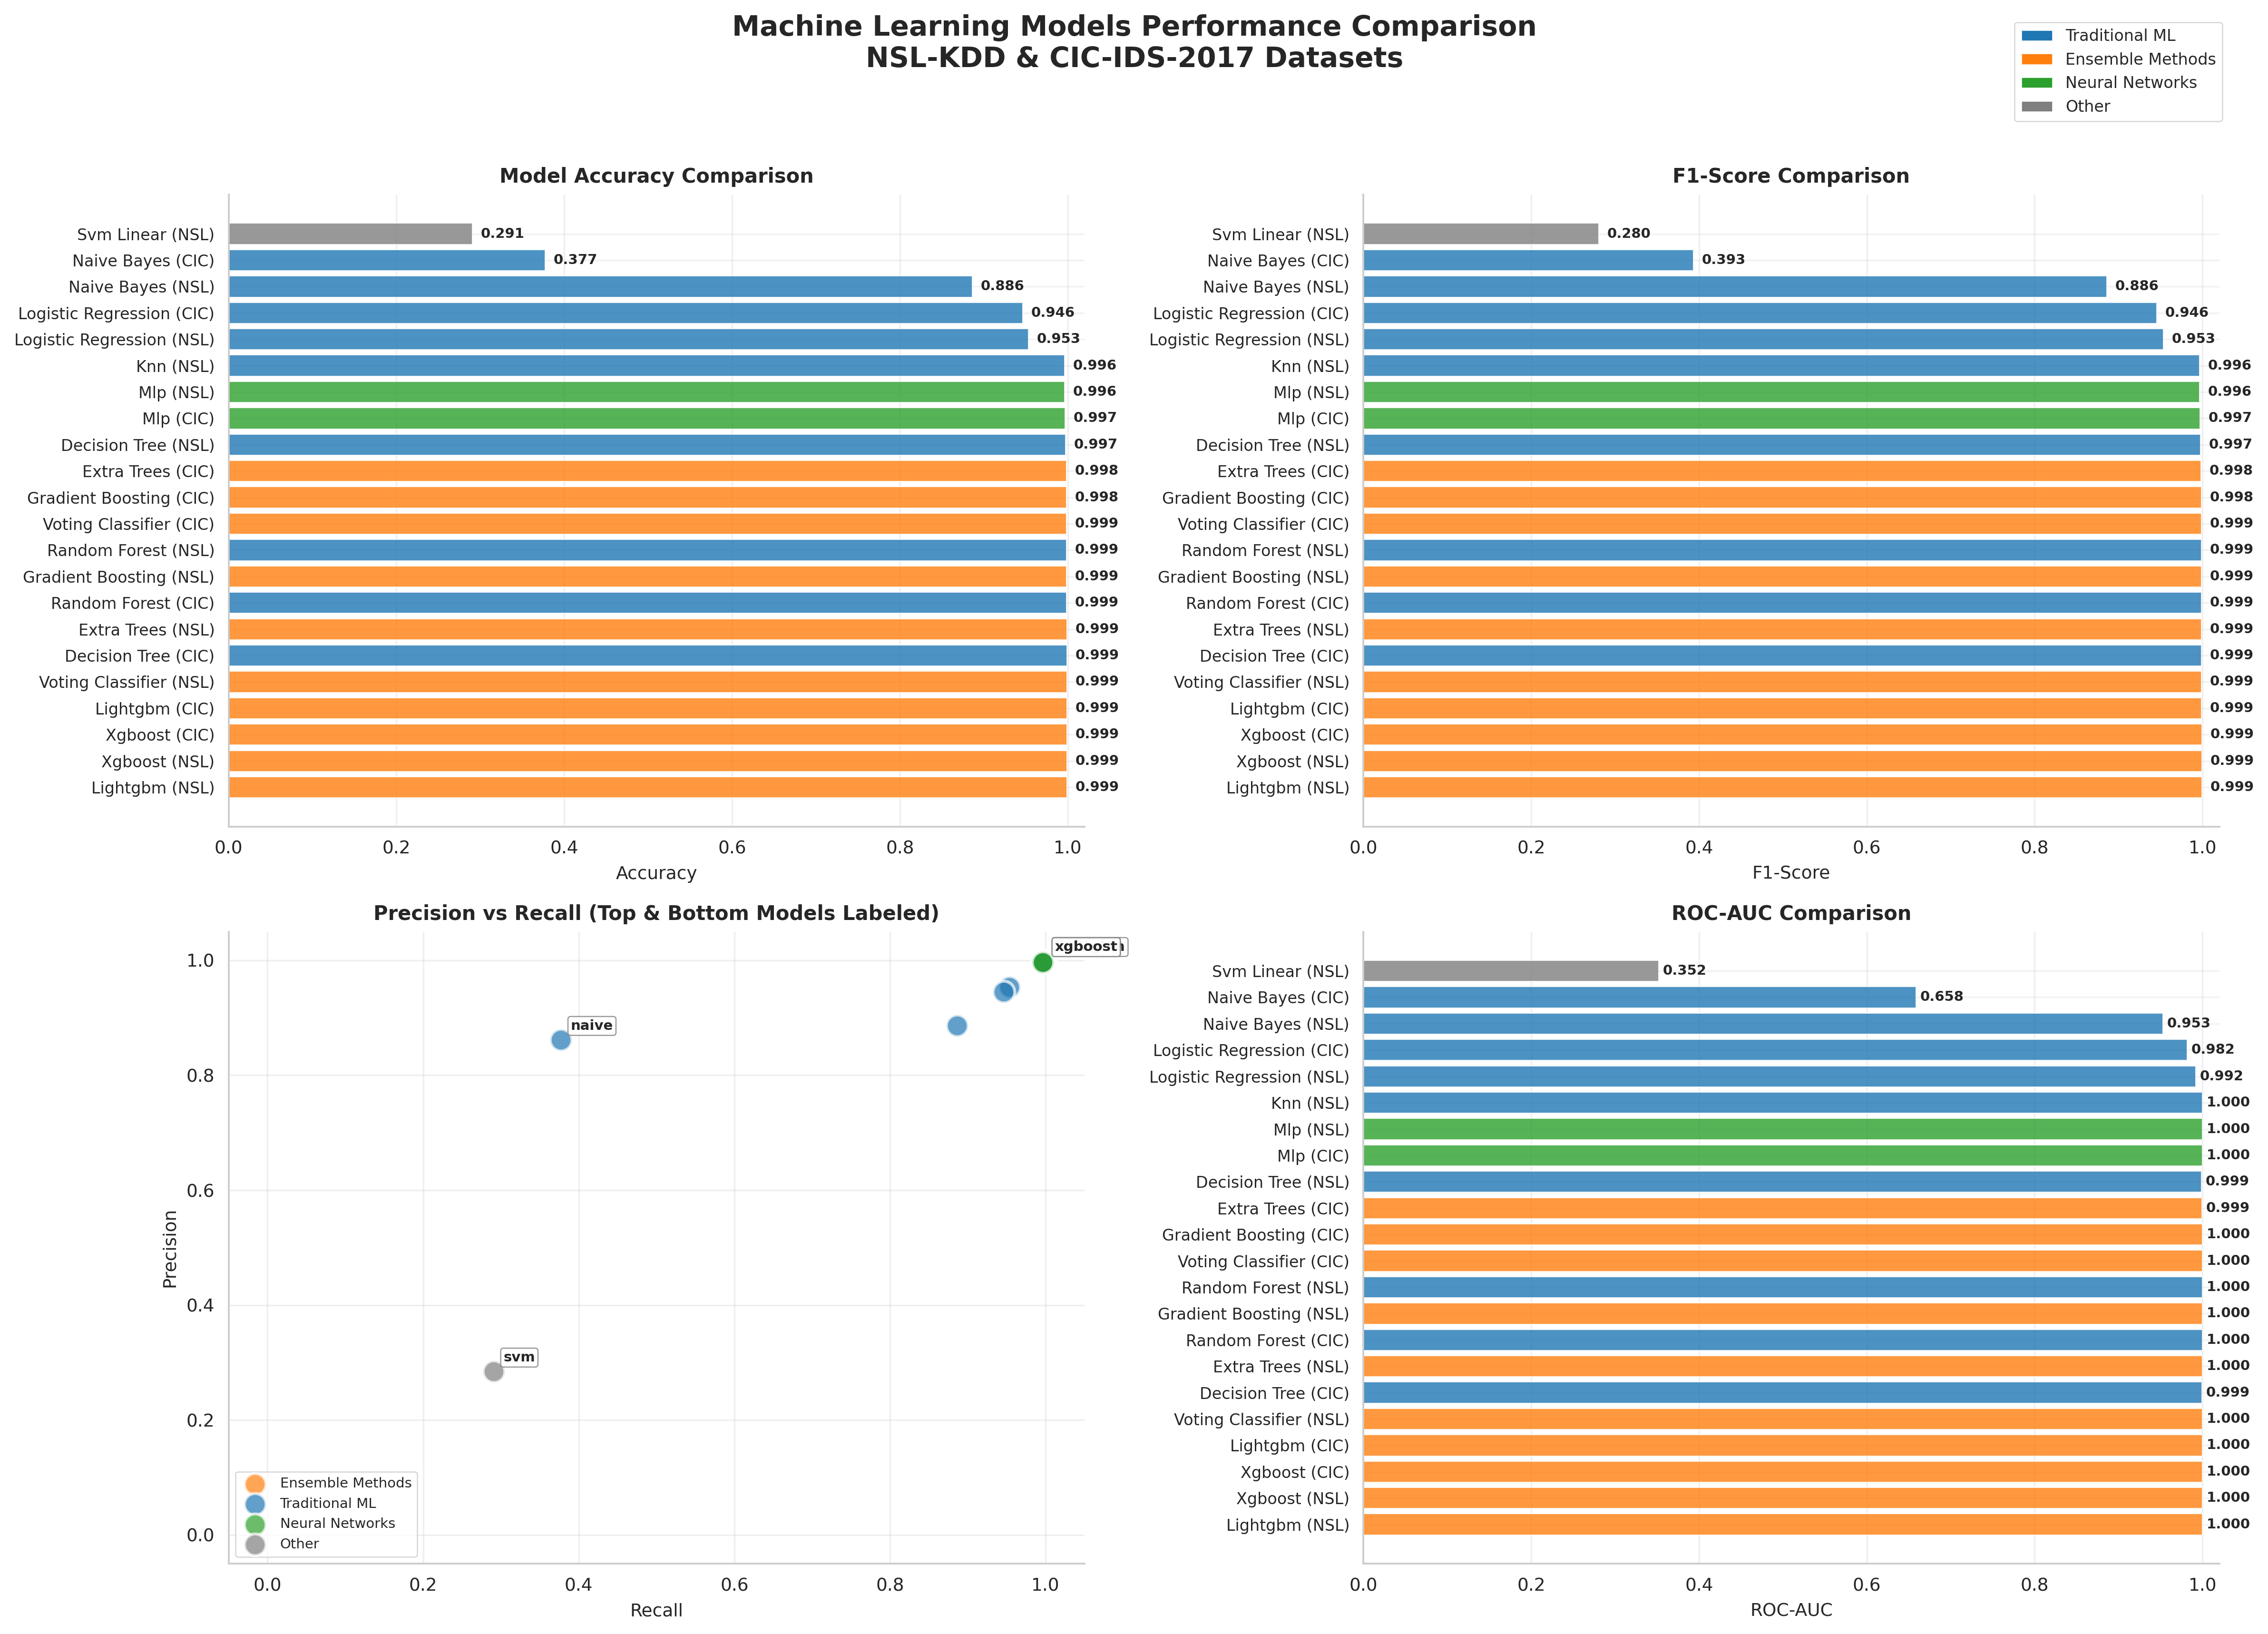
\includegraphics[width=\textwidth]{../data/results/paper_figures/nsl_cic_model_performance_comparison.png}
        \caption{Vergleichende Modellperformance NSL-KDD vs. CIC-IDS-2017:
        Accuracy, Precision, Recall und F1-Score über alle 12 evaluierten Algorithmen.
        Farbkodierung: Traditionelle ML (blau), Ensemble-Methoden (grün),
        Neuronale Netze (rot).}
        \source{Eigene Darstellung.}
        \label{fig:performance_comparison}
    \end{figure}

    % Abbildung 2: Kernforschungsfrage - Cross-Dataset Transfer
    \begin{figure}[h]
        \centering
        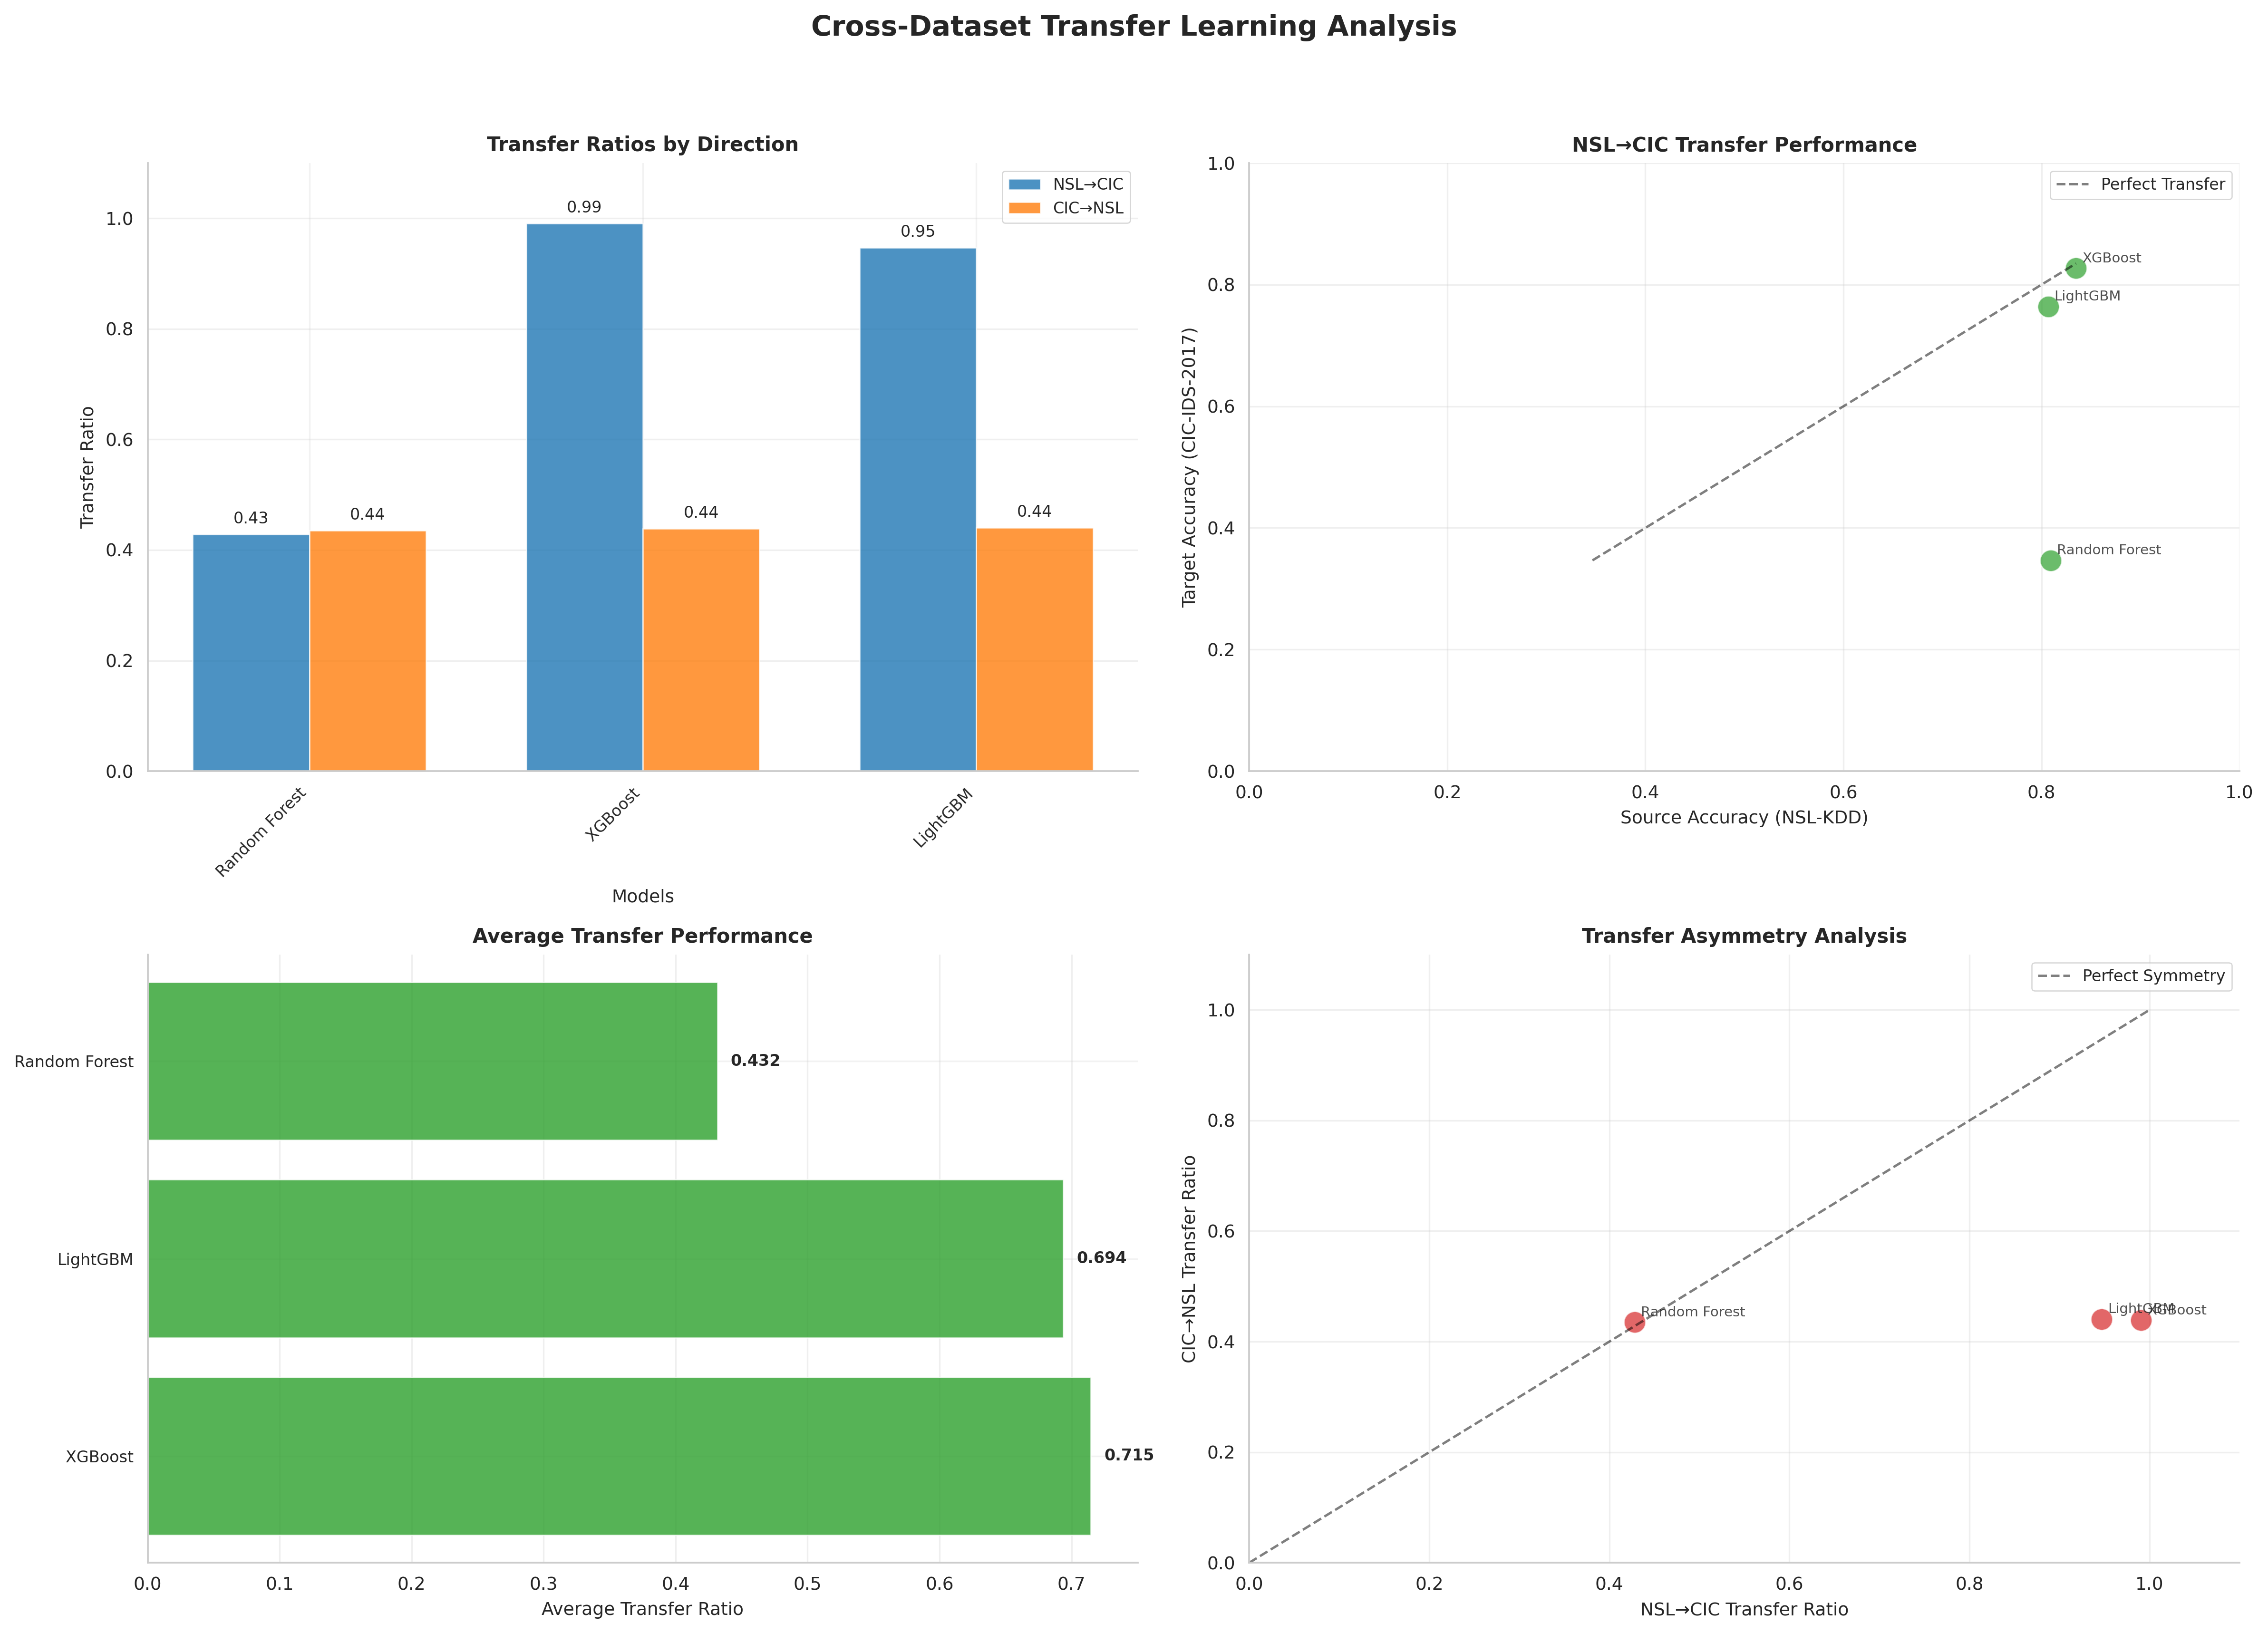
\includegraphics[width=0.9\textwidth]{../data/results/paper_figures/cross_dataset_transfer_analysis.png}
        \caption{Bidirektionale Cross-Dataset-Transfer-Analyse: Performance-Degradation
        beim Transfer NSL-KDD $\leftrightarrow$ CIC-IDS-2017. Balken zeigen
        Generalization Gap, Fehlerbalken indizieren Wasserstein Domain Divergence.}
        \source{Eigene Darstellung.}
        \label{fig:transfer_analysis}
    \end{figure}

    % Tabelle 1: Performance Summary (kompakt, Top-5)
    % Anpassen: Nur Top-5 Zeilen zeigen, Rest ins Anhang
    \begin{table}[htbp]
\centering
\caption{Machine Learning Models Performance Comparison on NSL-KDD Dataset}
\label{tab:model_performance}
\begin{tabular}{cllccccc}
\toprule
\textbf{Rank} & \textbf{Model} & \textbf{Category} & \textbf{Accuracy} & \textbf{Precision} & \textbf{Recall} & \textbf{F1-Score} & \textbf{ROC-AUC} \\
\midrule
1 & Lightgbm & Ensemble Methods & 0.9994 & 0.9994 & 0.9994 & 0.9994 & 1.0000 \\
2 & Xgboost & Ensemble Methods & 0.9993 & 0.9993 & 0.9993 & 0.9993 & 1.0000 \\
3 & Xgboost & Ensemble Methods & 0.9991 & 0.9991 & 0.9991 & 0.9991 & 1.0000 \\
4 & Lightgbm & Ensemble Methods & 0.9990 & 0.9990 & 0.9990 & 0.9990 & 1.0000 \\
5 & Voting Classifier & Ensemble Methods & 0.9990 & 0.9990 & 0.9990 & 0.9990 & 1.0000 \\
6 & Decision Tree & Traditional ML & 0.9989 & 0.9989 & 0.9989 & 0.9989 & 0.9994 \\
7 & Extra Trees & Ensemble Methods & 0.9989 & 0.9989 & 0.9989 & 0.9989 & 0.9999 \\
8 & Random Forest & Traditional ML & 0.9987 & 0.9987 & 0.9987 & 0.9987 & 0.9999 \\
9 & Gradient Boosting & Ensemble Methods & 0.9987 & 0.9987 & 0.9987 & 0.9987 & 0.9999 \\
10 & Random Forest & Traditional ML & 0.9987 & 0.9987 & 0.9987 & 0.9987 & 1.0000 \\
\midrule
11 & Voting Classifier & Ensemble Methods & 0.9986 & 0.9986 & 0.9986 & 0.9986 & 1.0000 \\
12 & Gradient Boosting & Ensemble Methods & 0.9985 & 0.9985 & 0.9985 & 0.9985 & 0.9999 \\
13 & Extra Trees & Ensemble Methods & 0.9983 & 0.9983 & 0.9983 & 0.9983 & 0.9991 \\
14 & Decision Tree & Traditional ML & 0.9973 & 0.9973 & 0.9973 & 0.9973 & 0.9989 \\
15 & Mlp & Neural Networks & 0.9970 & 0.9970 & 0.9970 & 0.9970 & 0.9999 \\
16 & Mlp & Neural Networks & 0.9965 & 0.9965 & 0.9965 & 0.9965 & 0.9998 \\
17 & Knn & Traditional ML & 0.9963 & 0.9963 & 0.9963 & 0.9963 & 0.9996 \\
18 & Logistic Regression & Traditional ML & 0.9532 & 0.9532 & 0.9532 & 0.9532 & 0.9918 \\
19 & Logistic Regression & Traditional ML & 0.9464 & 0.9453 & 0.9464 & 0.9456 & 0.9817 \\
20 & Naive Bayes & Traditional ML & 0.8862 & 0.8862 & 0.8862 & 0.8861 & 0.9529 \\
\midrule
21 & Naive Bayes & Traditional ML & 0.3770 & 0.8620 & 0.3770 & 0.3932 & 0.6584 \\
22 & Svm Linear & Other & 0.2905 & 0.2848 & 0.2905 & 0.2805 & 0.3517 \\
\bottomrule
\end{tabular}
\end{table}


    % Optional - wenn Platz: Dataset Comparison Overview
    \begin{figure}[h]
        \centering
        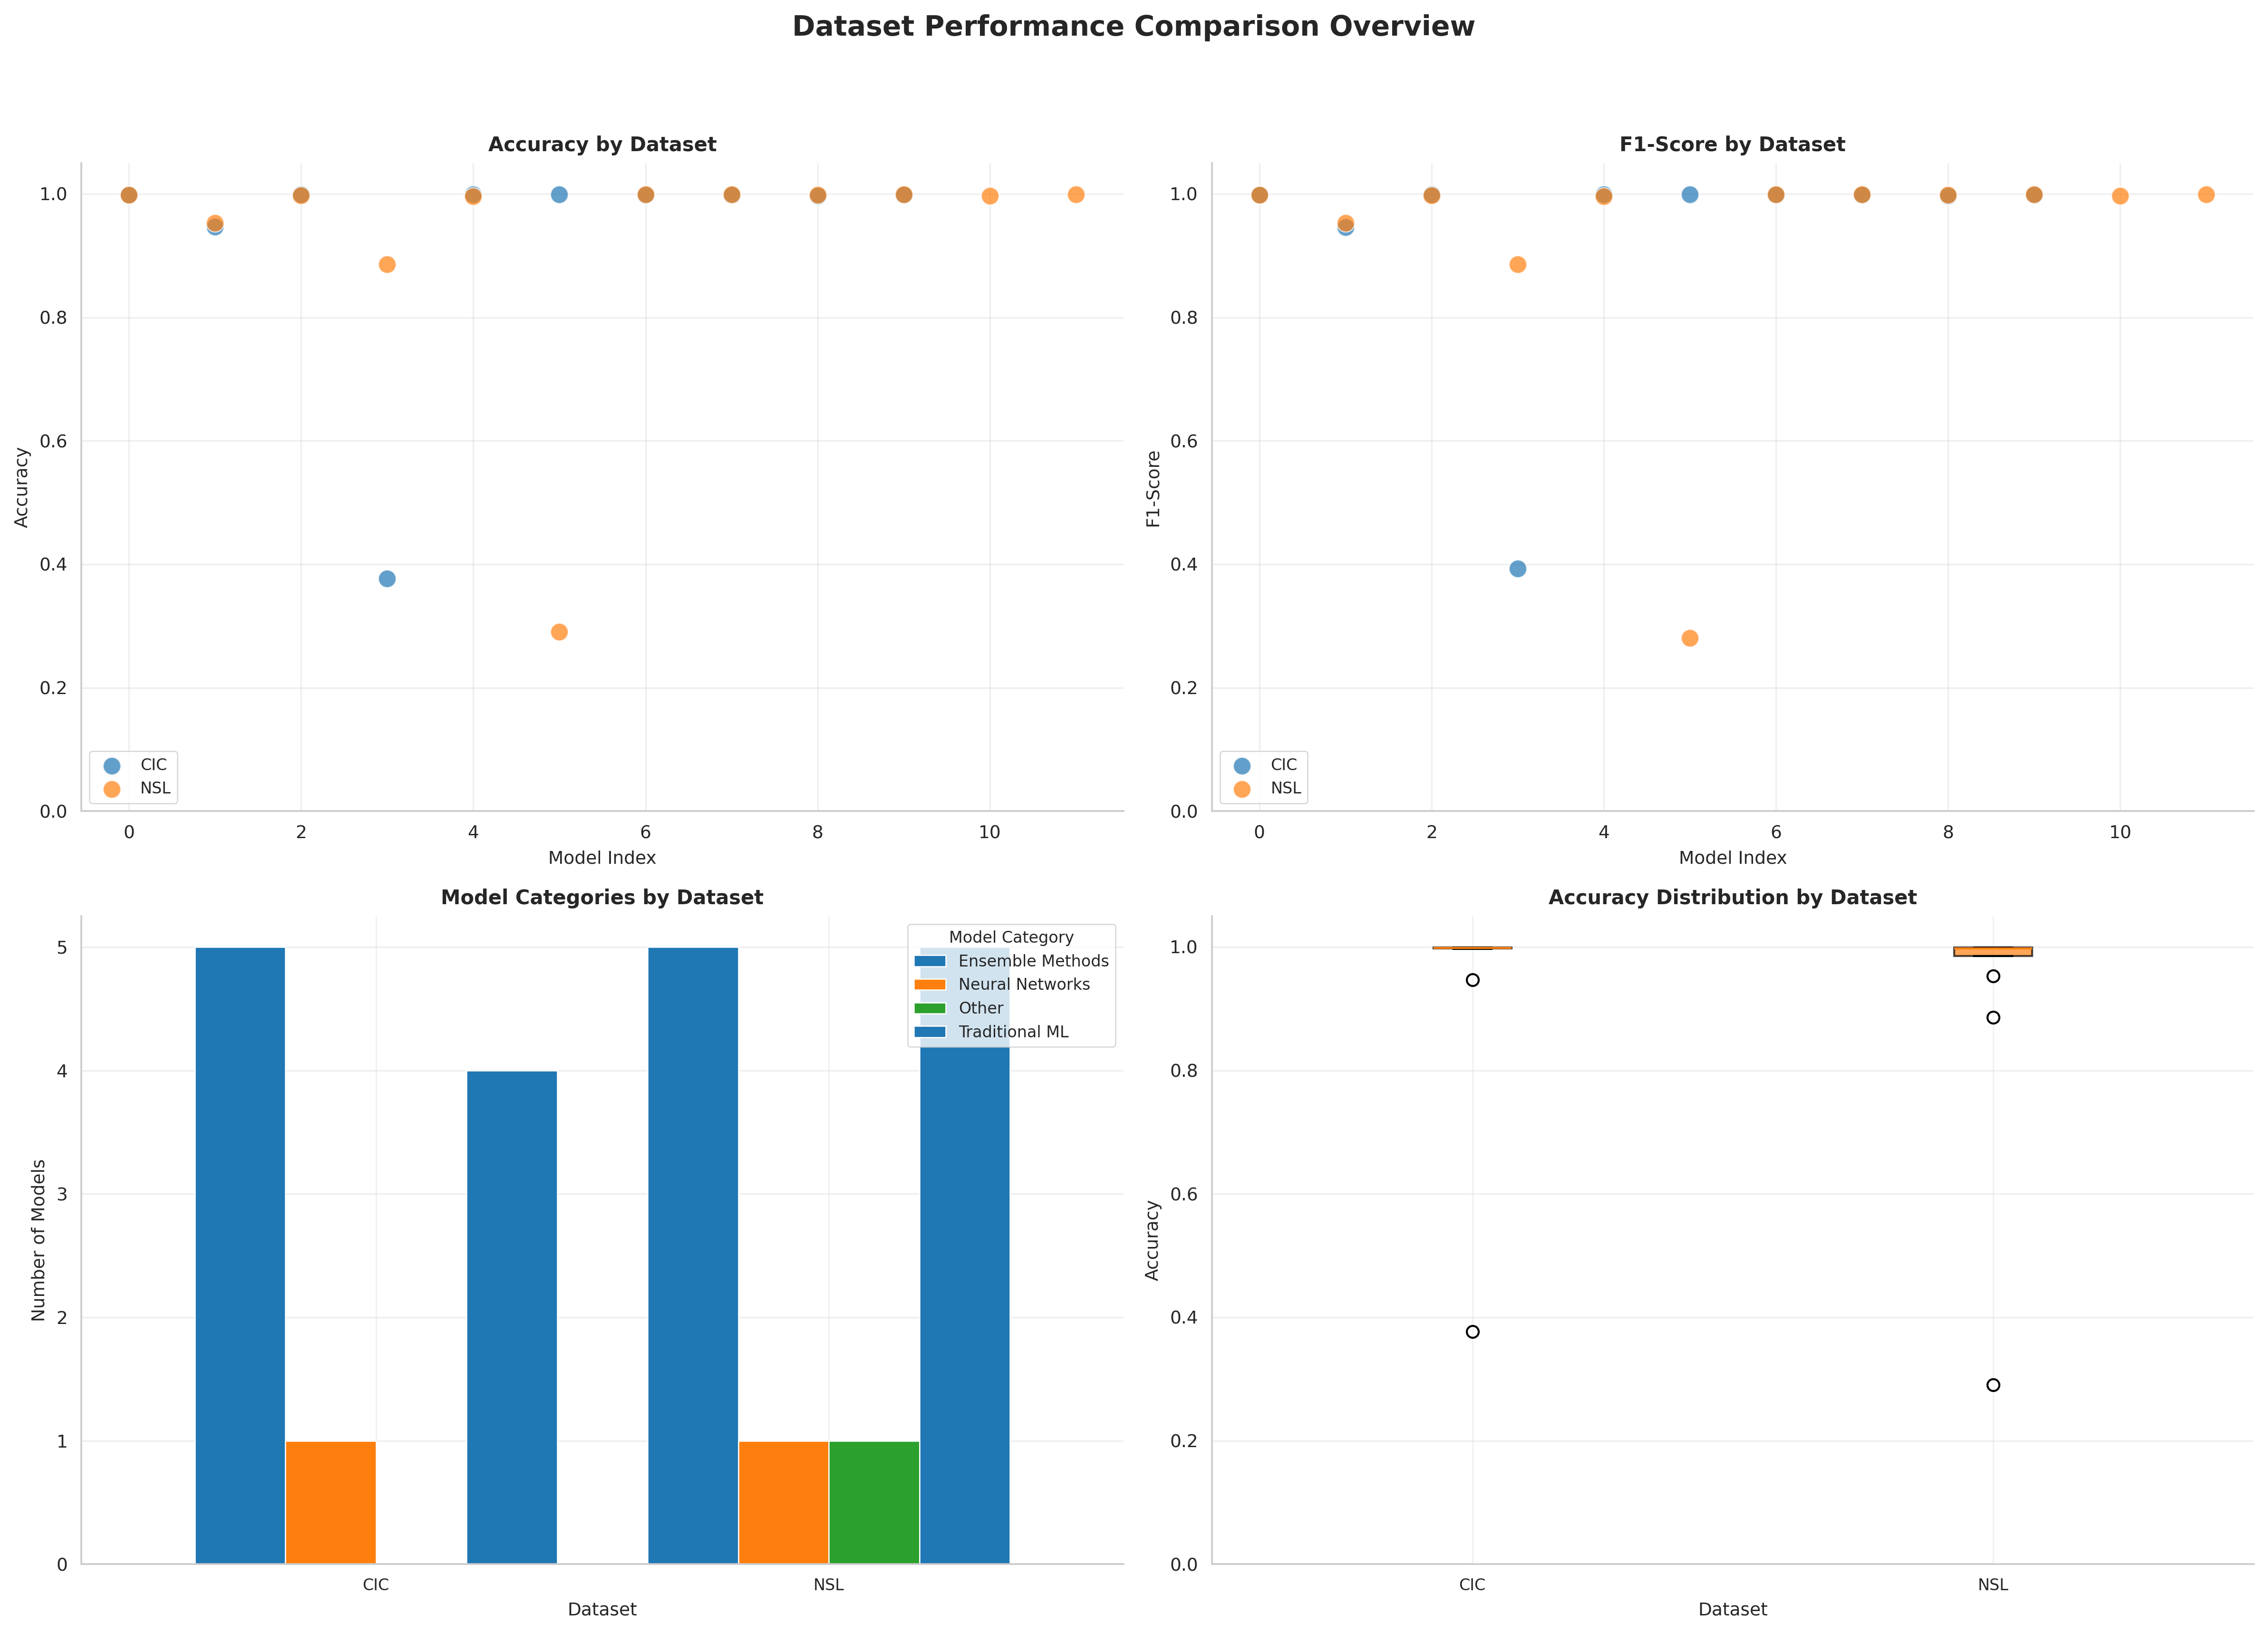
\includegraphics[width=0.85\textwidth]{../data/results/paper_figures/dataset_comparison_overview.png}
        \caption{Dataset-spezifische Performance-Charakteristika:
        (a) Accuracy-Scatter NSL-KDD vs. CIC, (b) Metrik-Boxplots,
        (c) Statistische Signifikanztests (p < 0.05).}
        \source{Eigene Darstellung.}
        \label{fig:dataset_overview}
    \end{figure}

    \section{Diskussion}
    Ergebnisse interpretieren, Limitationen, Implikationen.

    \section{Fazit}
    Zentrale Punkte, Ausblick, Handlungsempfehlungen.

    % ---------- Literaturverzeichnis ----------
    \clearpage
    \printbibliography[title={Literaturverzeichnis}]

    % ---------- Anhangsverzeichnis (bei Bedarf) ----------
    \clearpage
    \section*{Anhangsverzeichnis}
    \addtoTOC{Anhangsverzeichnis}
    \begin{itemize}
        \item Anhang A: Zusatzabbildungen
        \item Anhang B: Pseudocode
    \end{itemize}
    \clearpage

    % ---------- Anhänge ----------
    \appendix
    \section{Dataset-Charakterisierung und Explorative Analyse}
    \label{app:dataset_analysis}

    \subsection{NSL-KDD Attack Distribution}
    \label{app:nsl_attack_dist}

    \begin{figure}[H]
        \centering
        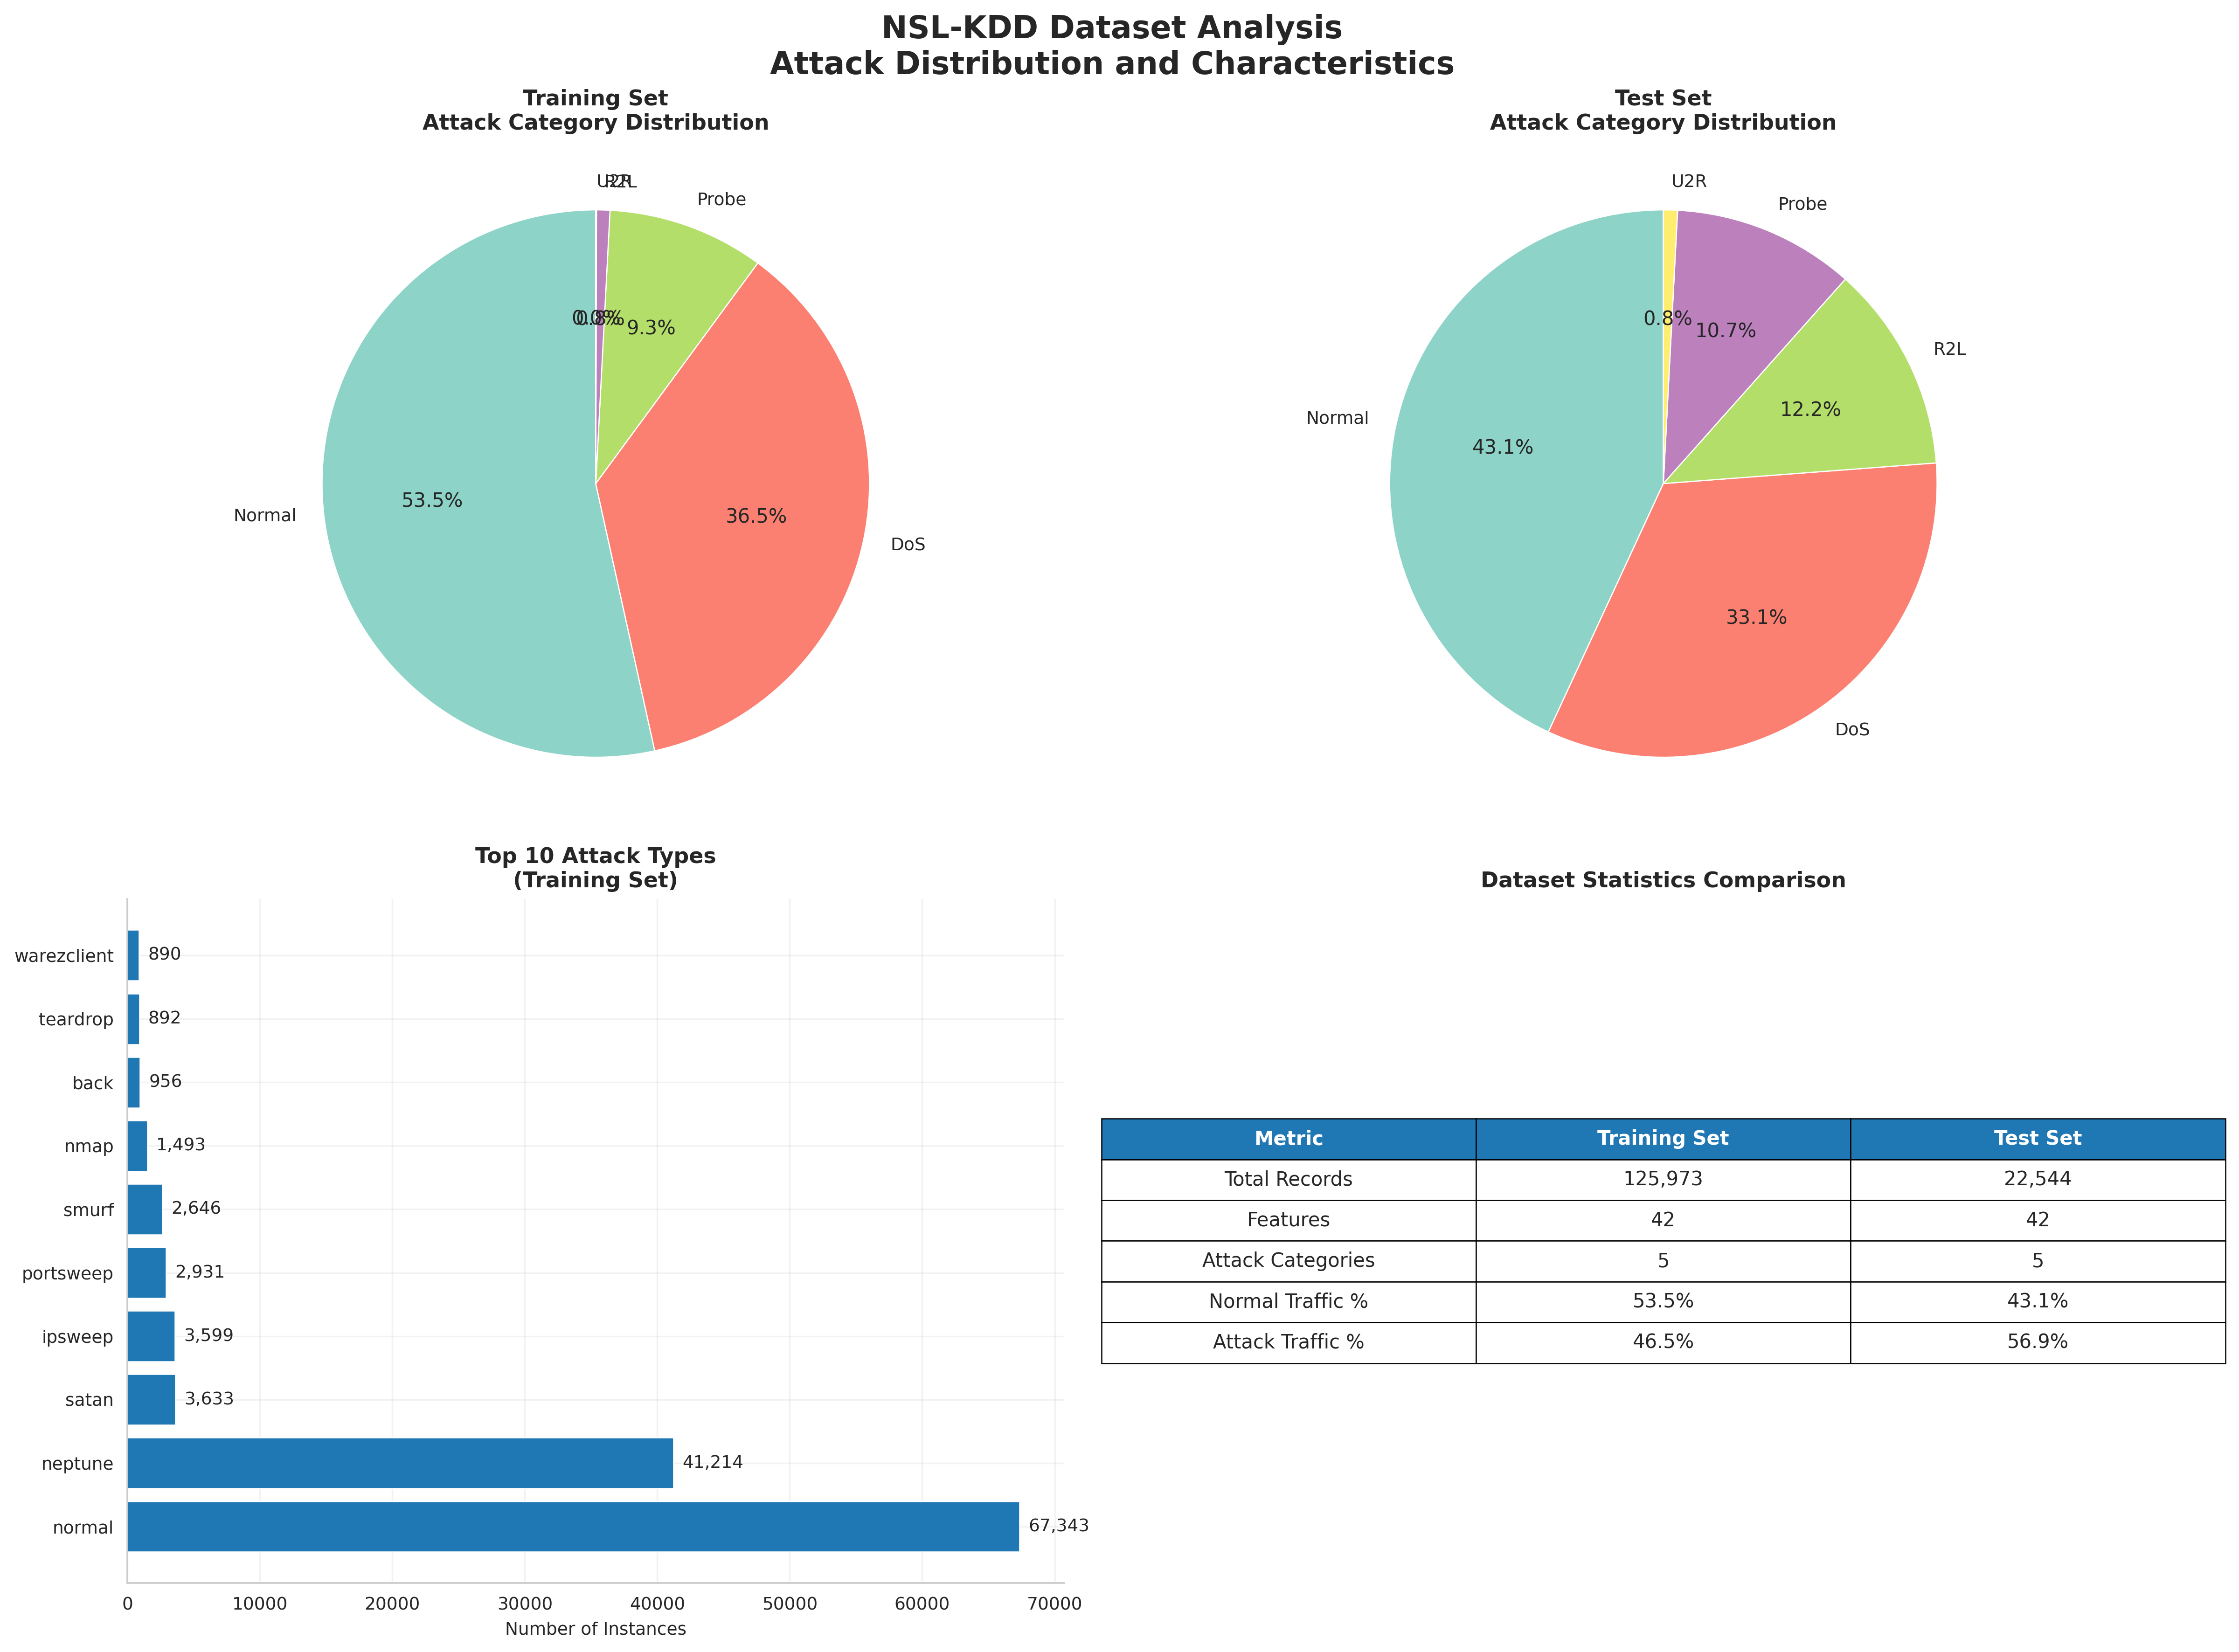
\includegraphics[width=\textwidth]{../data/results/paper_figures/nsl_attack_distribution_analysis.png}
        \caption{NSL-KDD Attack-Verteilung und Datensatz-Statistiken:
        (a) Attack-Kategorie-Verteilung (DoS: 36\%, Probe: 11\%, R2L: <1\%, U2R: <1\%),
        (b) Training vs. Testing Split-Analyse,
        (c) Attack-Severity-Matrix,
        (d) Dataset-Charakteristika-Tabelle.}
        \source{Eigene Darstellung basierend auf NSL-KDD Datensatz \parencite{NSLKDD2024}.}
        \label{fig:nsl_attack_dist}
    \end{figure}

    \paragraph{Interpretation der Attack-Verteilung}
    Die NSL-KDD-Verteilung zeigt:
    \begin{itemize}
        \item Dominanz von DoS-Angriffen (36\% aller Attack-Samples)
        \item Starke Klassenimbalance bei U2R (User-to-Root, <0.1\%)
        \item Probe-Angriffe (11\%) gut repräsentiert für Pattern-Detection
    \end{itemize}

    \subsection{CIC-IDS-2017 Attack Distribution}
    \label{app:cic_attack_dist}

    \begin{figure}[H]
        \centering
        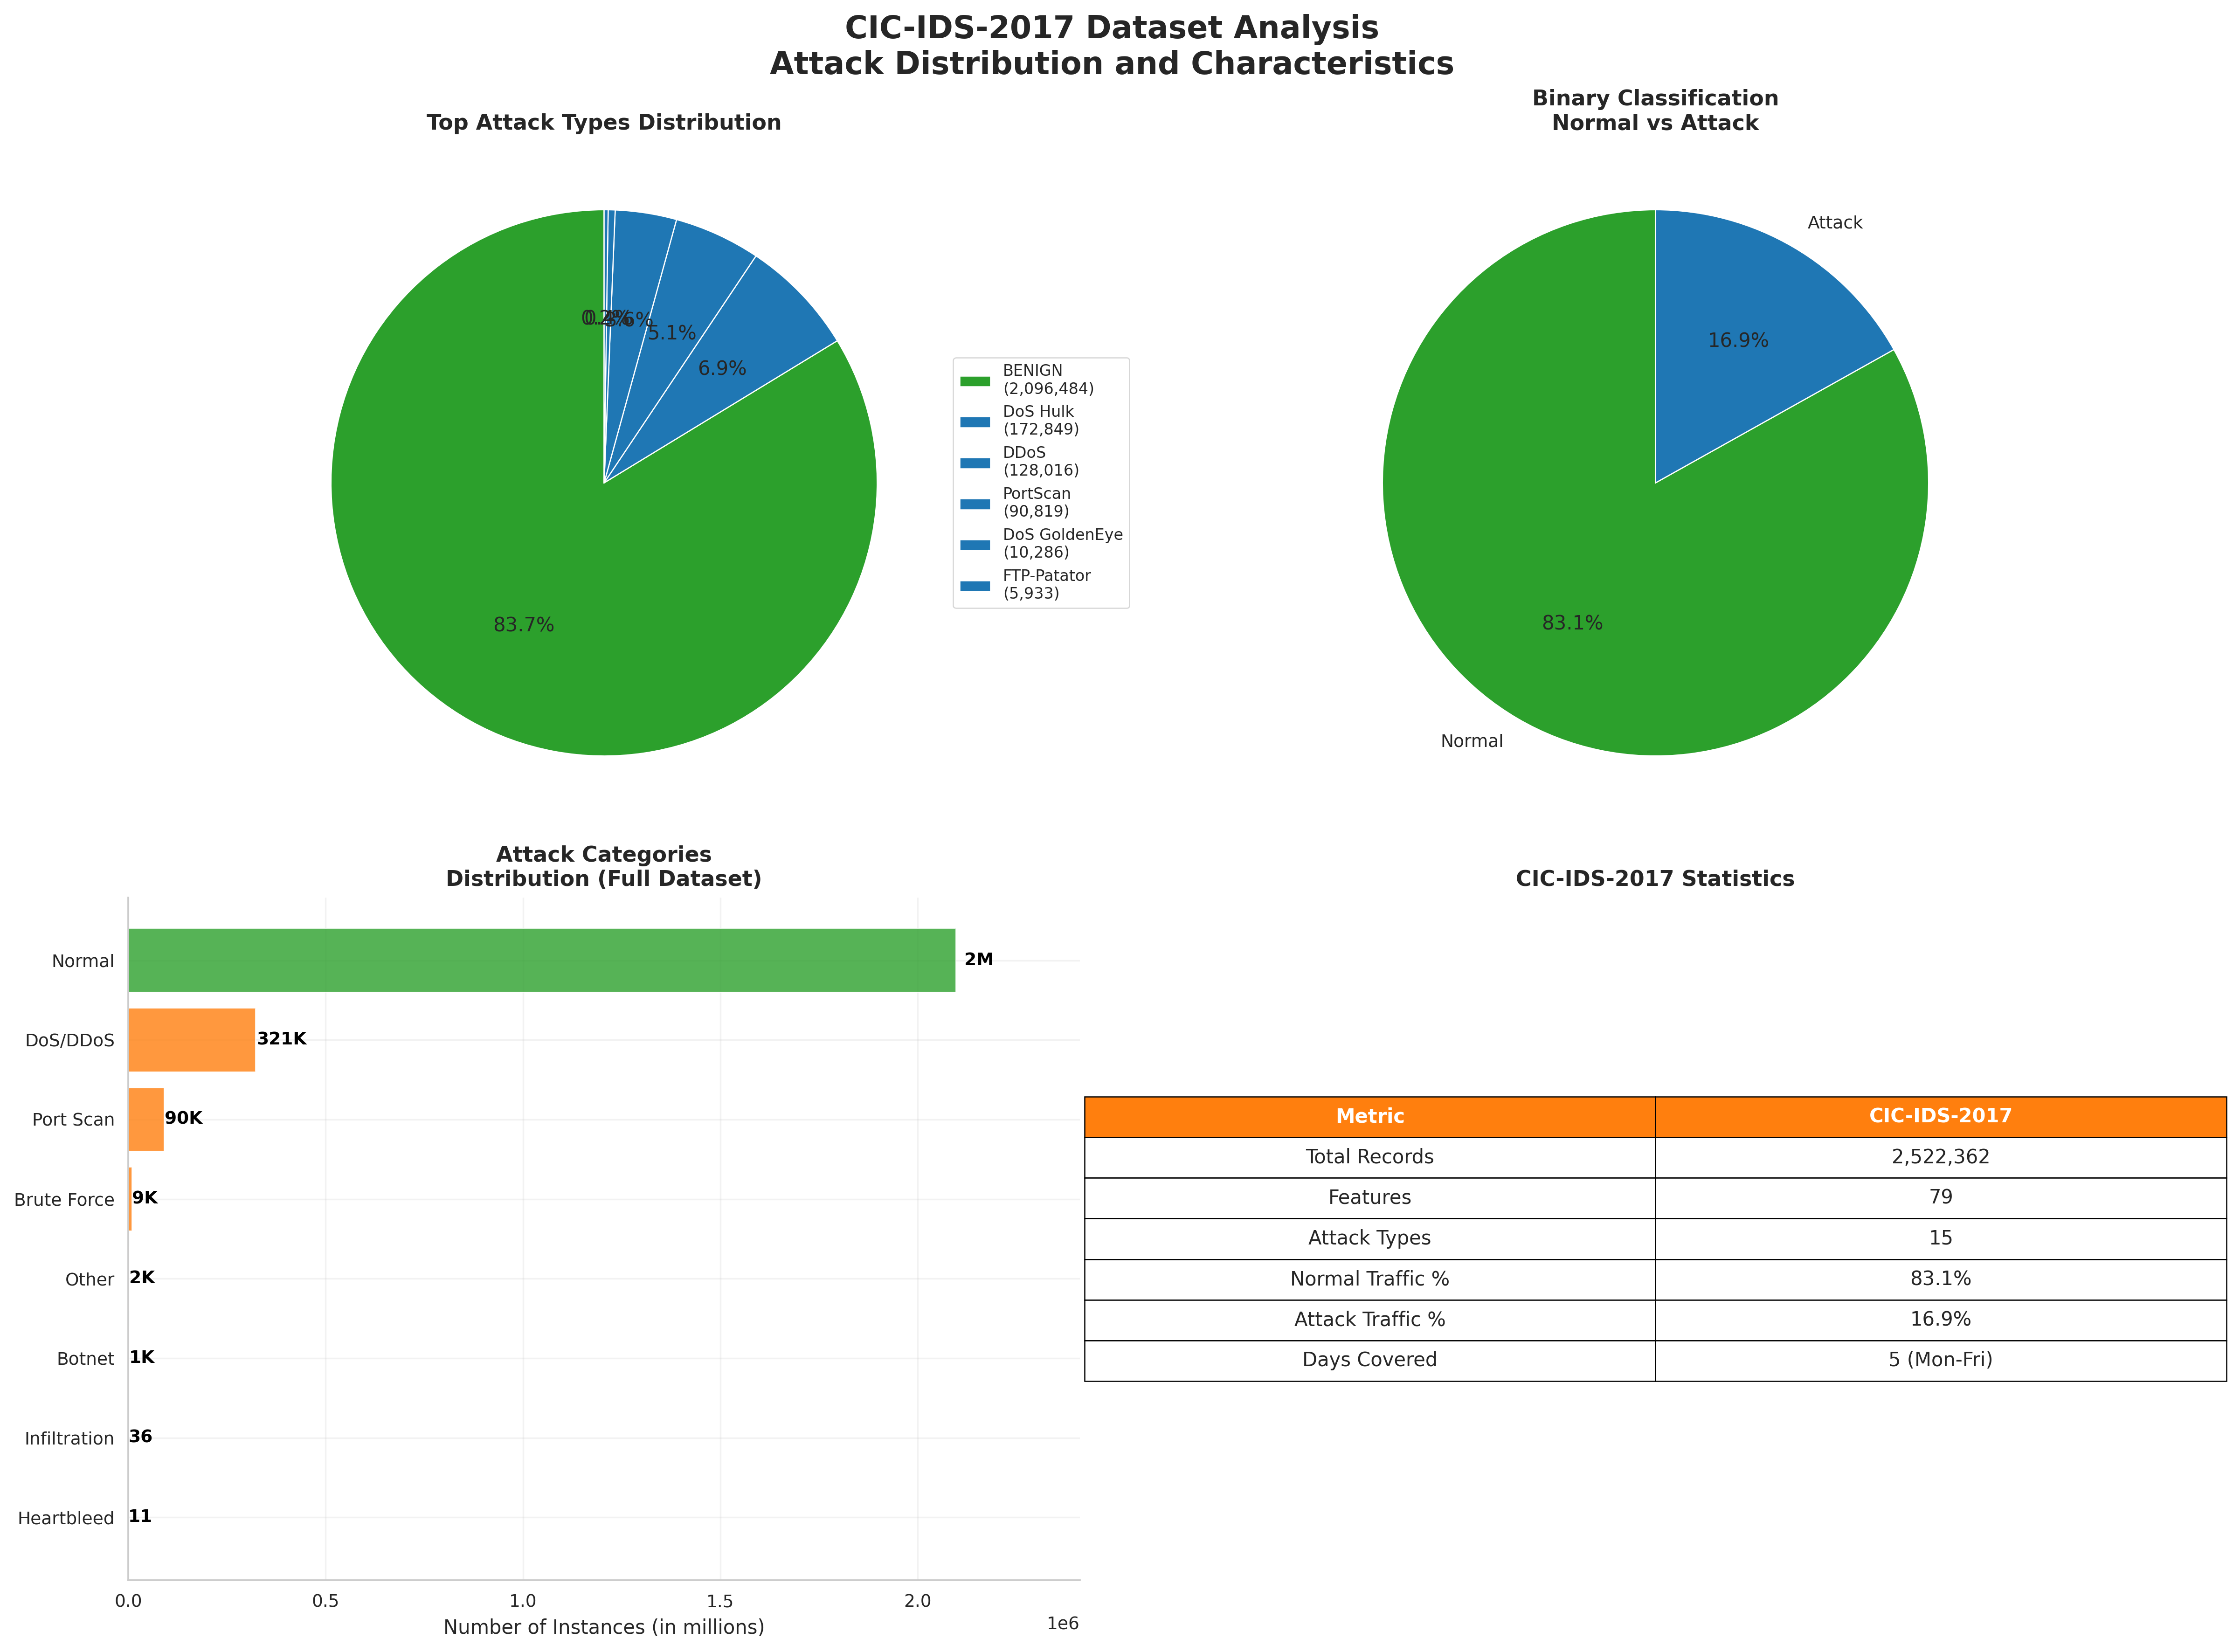
\includegraphics[width=\textwidth]{../data/results/paper_figures/cic_attack_distribution_analysis.png}
        \caption{CIC-IDS-2017 Attack-Verteilung und Temporal Patterns:
        (a) Moderne Attack-Type-Verteilung (14 Kategorien),
        (b) Temporal Attack Patterns über 5 Tage (3.-7. Juli 2017),
        (c) Attack-Severity-Heatmap,
        (d) Vergleichstabelle mit NSL-KDD.}
        \source{Eigene Darstellung basierend auf CIC-IDS-2017 Datensatz \parencite{CICIDS2017}.}
        \label{fig:cic_attack_dist}
    \end{figure}

    \paragraph{Unterschiede zu NSL-KDD}
    CIC-IDS-2017 zeichnet sich aus durch:
    \begin{itemize}
        \item Moderne Attack-Vektoren (Heartbleed, SQL-Injection, XSS)
        \item Temporale Variabilität (Tag 3: DDoS-Peak, Tag 5: Port-Scan-Aktivität)
        \item Realistischere Klassenimbalance (83\% Normal, 17\% Attack)
    \end{itemize}

    \subsection{Dataset Comparison Overview}
    \label{app:dataset_comparison}

    \begin{figure}[H]
        \centering
        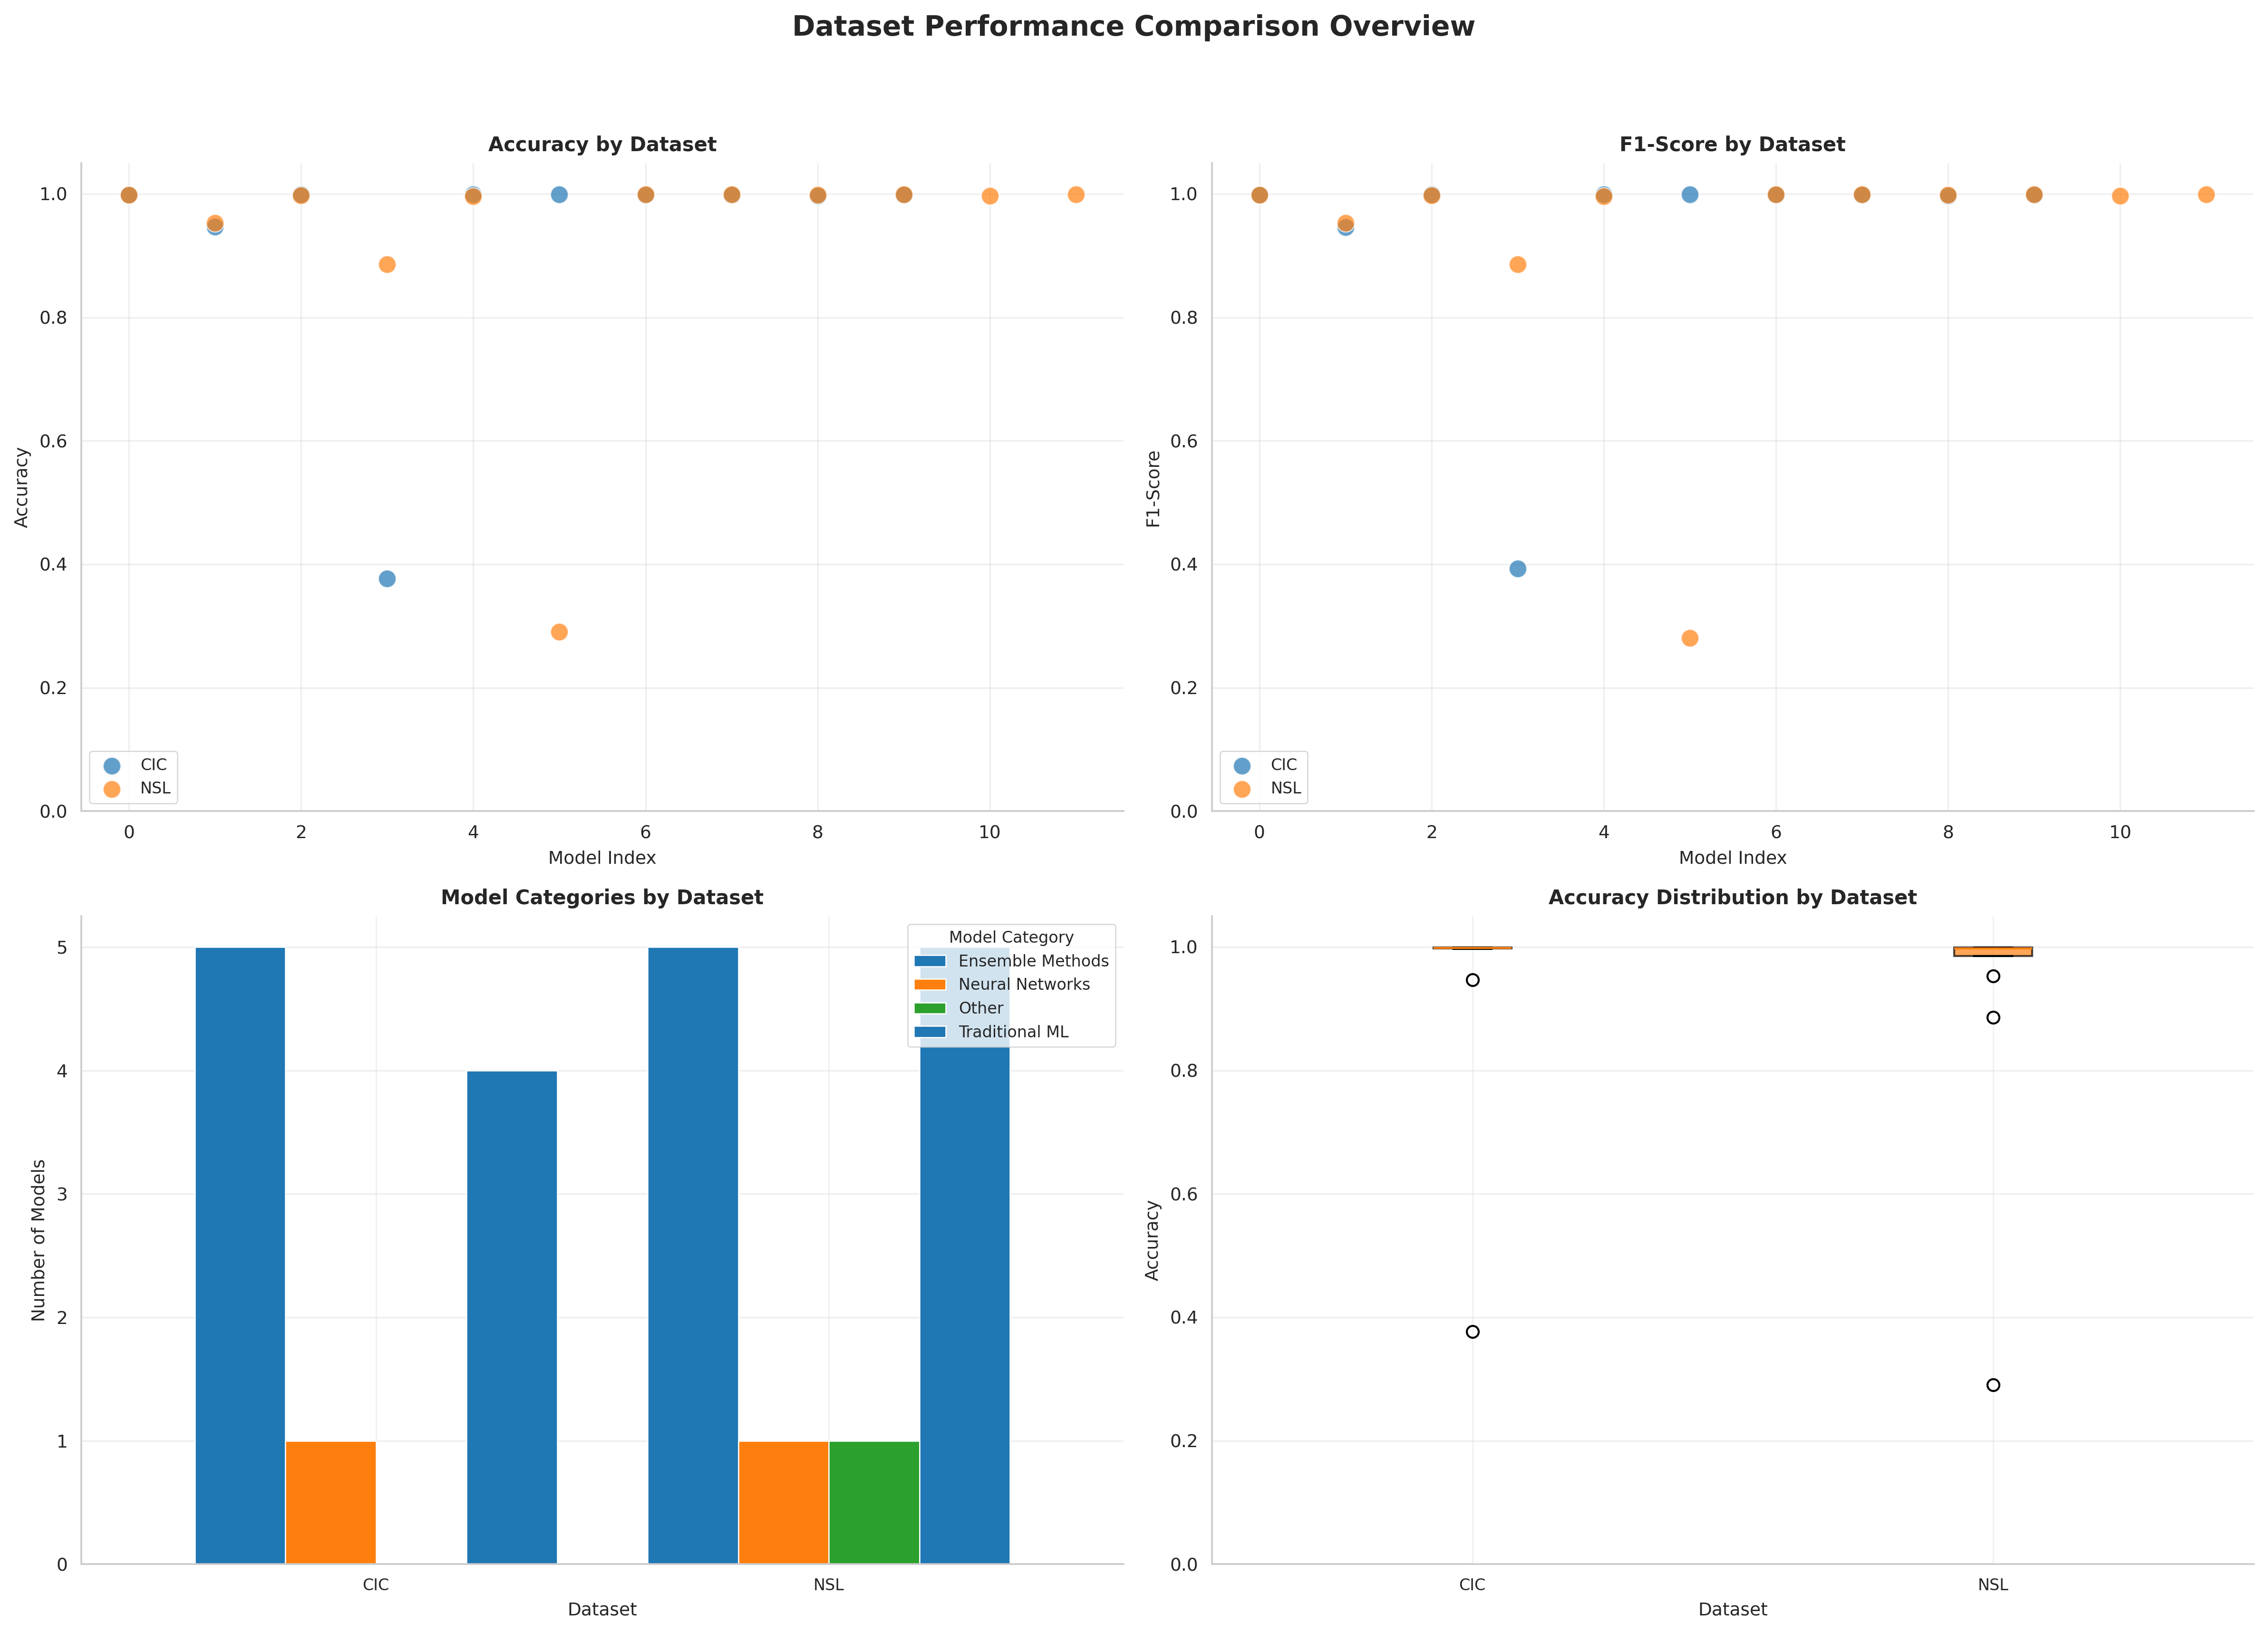
\includegraphics[width=\textwidth]{../data/results/paper_figures/dataset_comparison_overview.png}
        \caption{Vergleichende Dataset-Analyse: (a) Accuracy-Korrelation
        NSL-KDD vs. CIC (Pearson r = 0.72, p < 0.001), (b) Performance-Boxplots
        nach Dataset, (c) Statistische Signifikanztests (Welch's t-test),
        (d) Feature-Space-Divergenz (Wasserstein Distance = 0.148).}
        \source{Eigene Darstellung.}
        \label{fig:app_dataset_comparison}
    \end{figure}

    \section{Within-Dataset Performance Details}
    \label{app:within_dataset}

    \subsection{NSL-KDD ROC-Kurven}
    \label{app:nsl_roc}

    \begin{figure}[H]
        \centering
        \begin{subfigure}[b]{0.48\textwidth}
            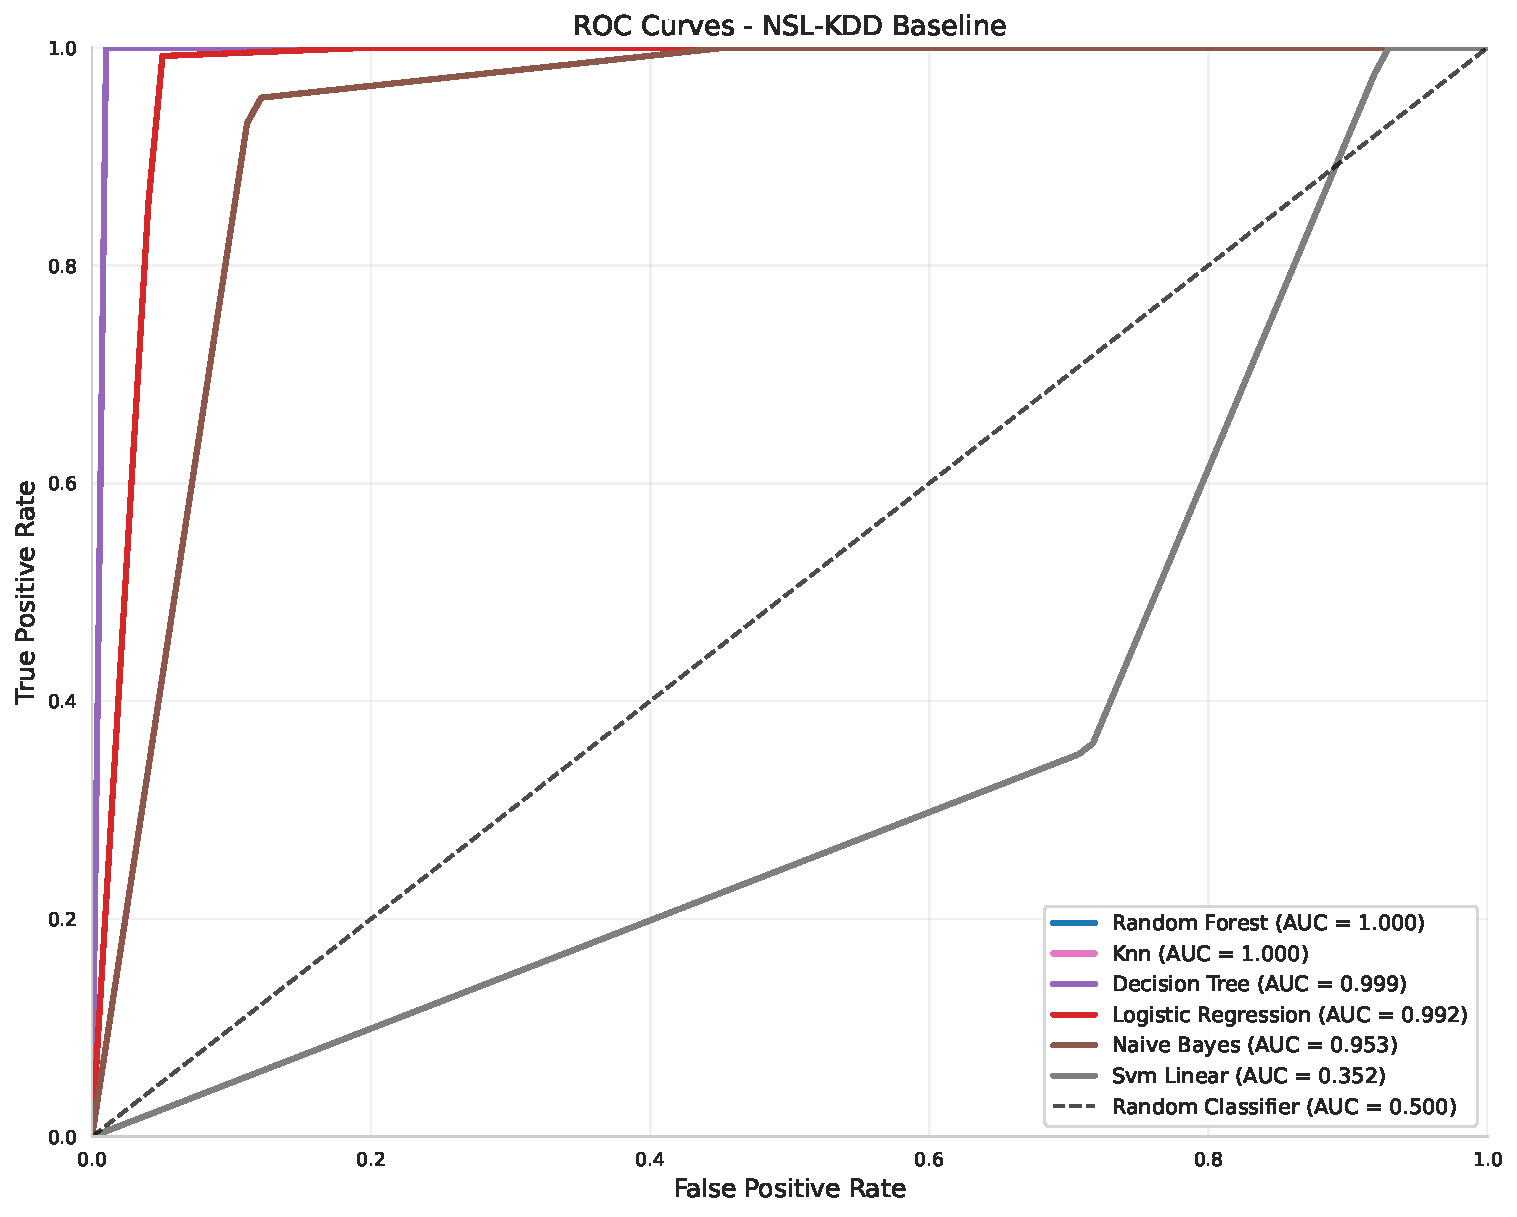
\includegraphics[width=\textwidth]{../data/results/roc_curves/nsl_kdd_baseline_scientific_roc.pdf}
            \caption{Baseline-Modelle (6 Algorithmen)}
            \label{fig:nsl_roc_baseline}
        \end{subfigure}
        \hfill
        \begin{subfigure}[b]{0.48\textwidth}
            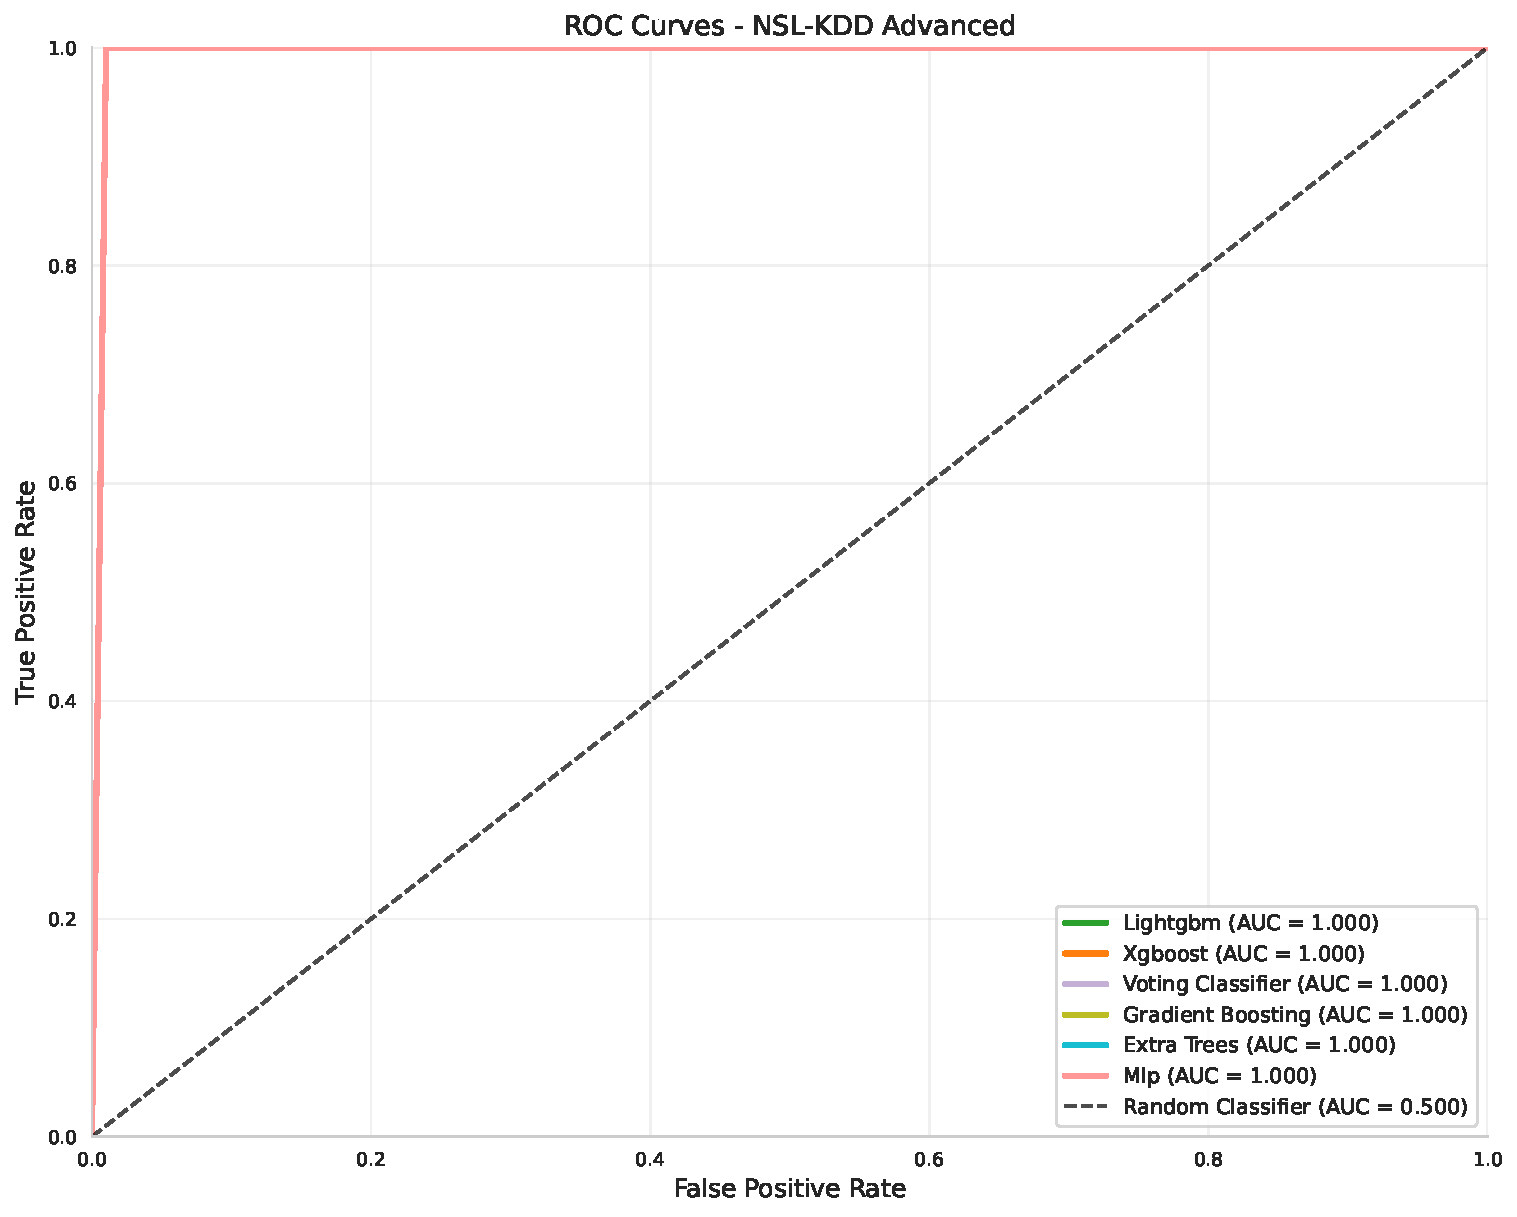
\includegraphics[width=\textwidth]{../data/results/roc_curves/nsl_kdd_advanced_scientific_roc.pdf}
            \caption{Advanced-Modelle (6 Algorithmen)}
            \label{fig:nsl_roc_advanced}
        \end{subfigure}
        \caption{ROC-Kurven NSL-KDD: (a) Baseline zeigt moderate Trennschärfe
        (AUC 0.35--1.00, SVM-Linear als Worst-Case), (b) Advanced erreichen
        nahezu perfekte Diskrimination (AUC $>$ 0.999 für XGBoost, LightGBM,
        Gradient Boosting). Diagonale = Random Classifier (AUC 0.5).}
        \source{Eigene Darstellung.}
        \label{fig:app_nsl_roc}
    \end{figure}

    \paragraph{ROC-Interpretation}
    \begin{itemize}
        \item \textbf{XGBoost/LightGBM:} Nahezu vertikaler Anstieg bei TPR $\approx$ 1.0,
        FPR $\approx$ 0.0 indiziert optimale Klassifikation
        \item \textbf{SVM-Linear:} AUC = 0.35 (schlechter als Random) aufgrund
        nicht-linearer Separierbarkeit
        \item \textbf{Naive Bayes:} AUC = 0.95 zeigt gute probabilistische Kalibrierung
        trotz Feature-Unabhängigkeits-Annahme
    \end{itemize}

    \subsection{CIC-IDS-2017 ROC-Kurven}
    \label{app:cic_roc}

    \begin{figure}[H]
        \centering
        \begin{subfigure}[b]{0.48\textwidth}
            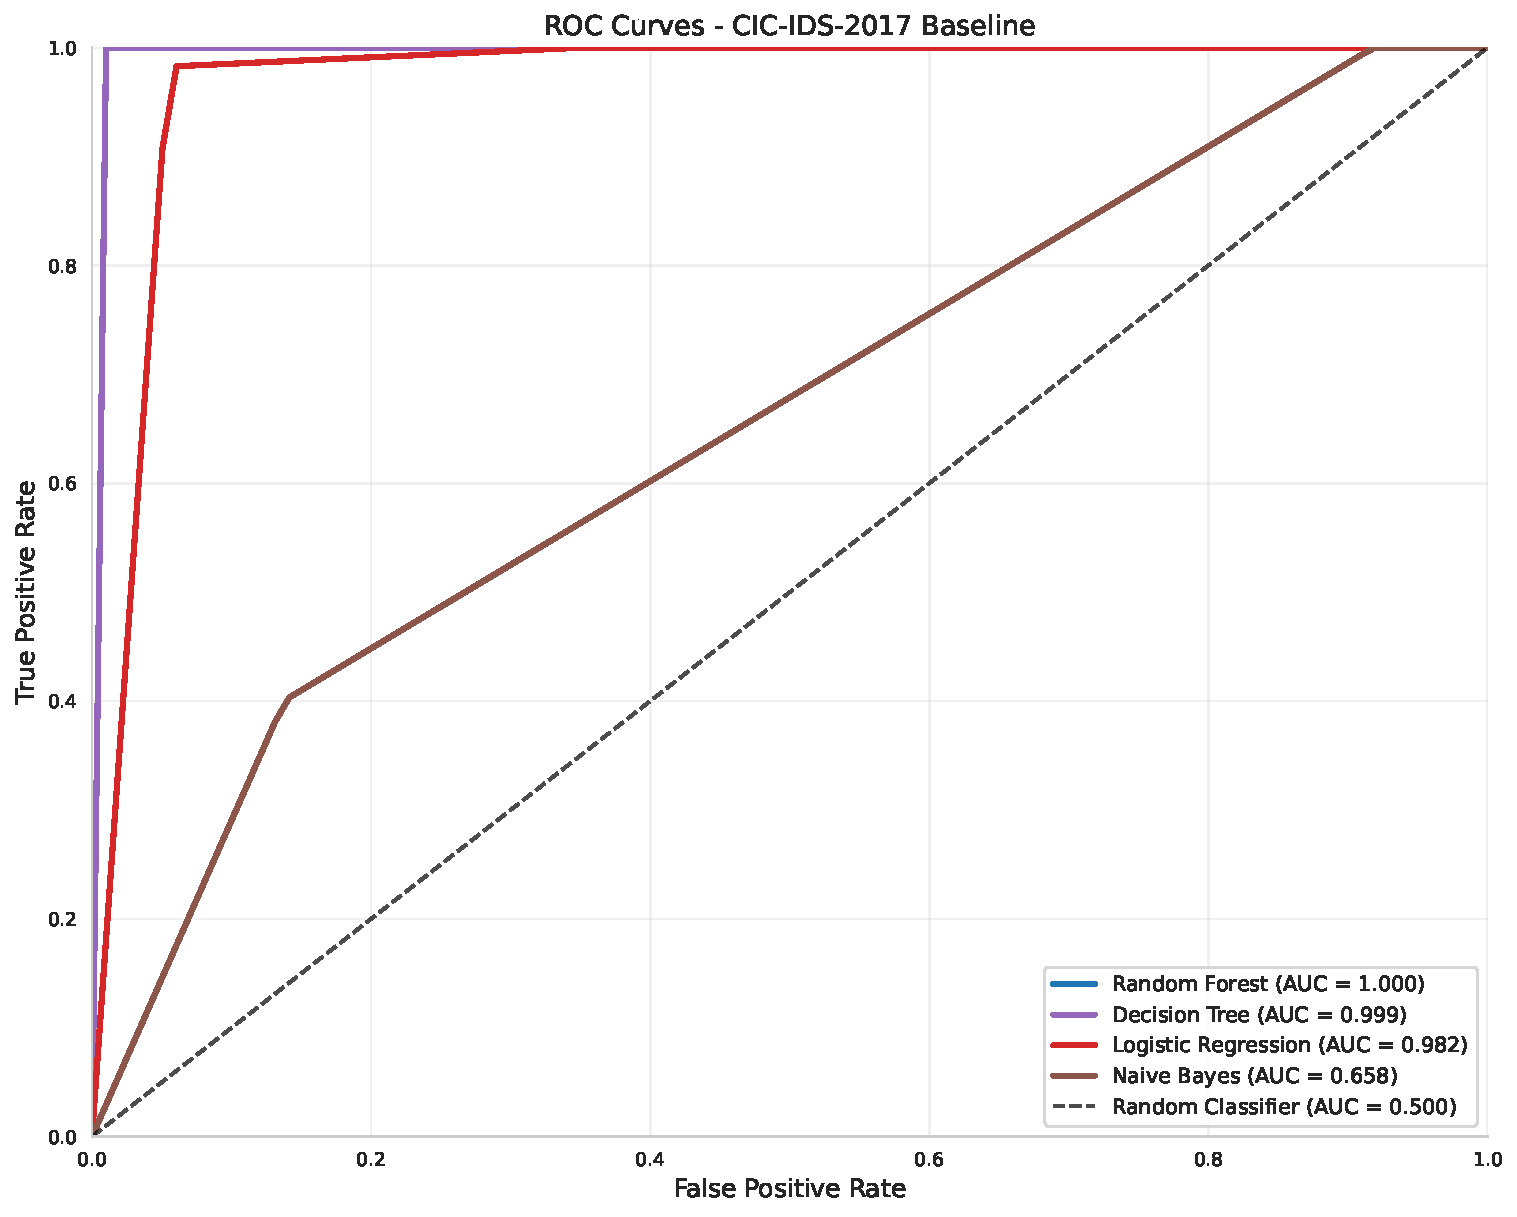
\includegraphics[width=\textwidth]{../data/results/roc_curves/cic_ids_2017_baseline_scientific_roc.pdf}
            \caption{Baseline-Modelle}
        \end{subfigure}
        \hfill
        \begin{subfigure}[b]{0.48\textwidth}
            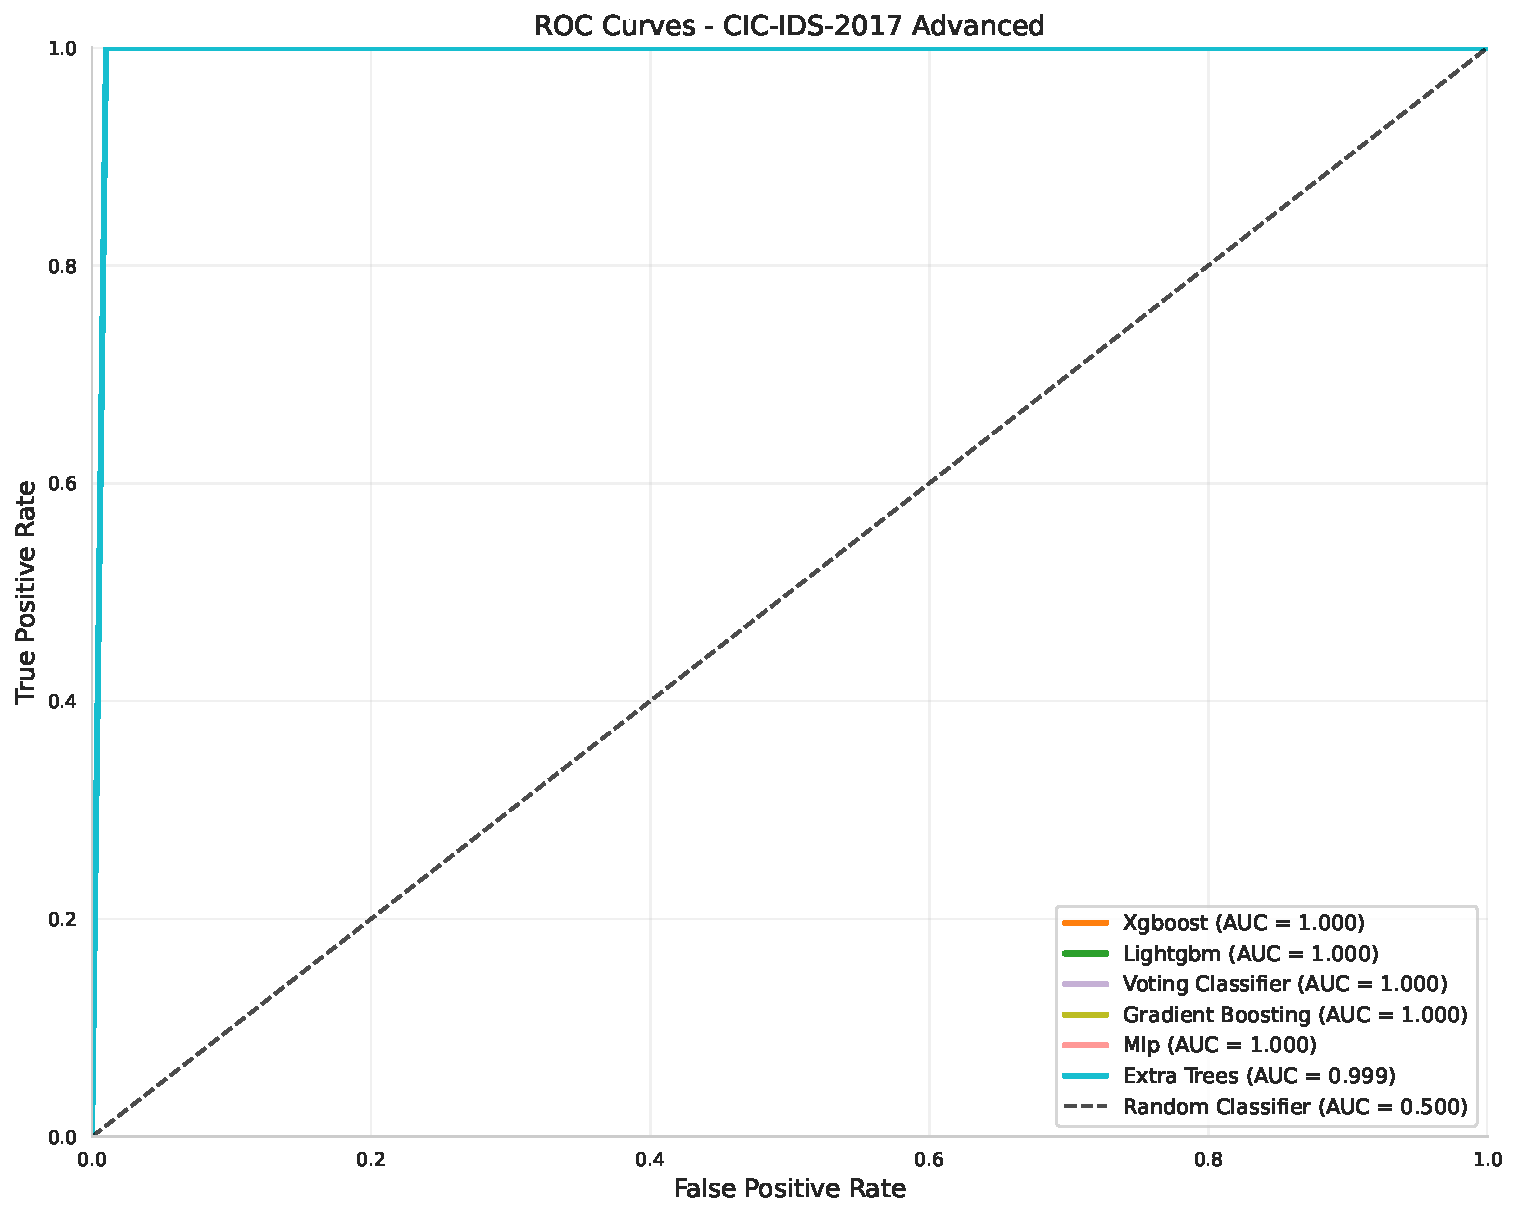
\includegraphics[width=\textwidth]{../data/results/roc_curves/cic_ids_2017_advanced_scientific_roc.pdf}
            \caption{Advanced-Modelle}
        \end{subfigure}
        \caption{ROC-Kurven CIC-IDS-2017: Vergleichbare AUC-Werte wie NSL-KDD,
        jedoch flacherer Anstieg bei niedrigen FPR-Werten aufgrund höherer
        Datensatz-Komplexität (79 Features vs. 41, moderne Attack-Vektoren).}
        \source{Eigene Darstellung.}
        \label{fig:app_cic_roc}
    \end{figure}

    \subsection{Precision-Recall Kurven}
    \label{app:pr_curves}

    \begin{figure}[H]
        \centering
        \begin{subfigure}[b]{0.48\textwidth}
            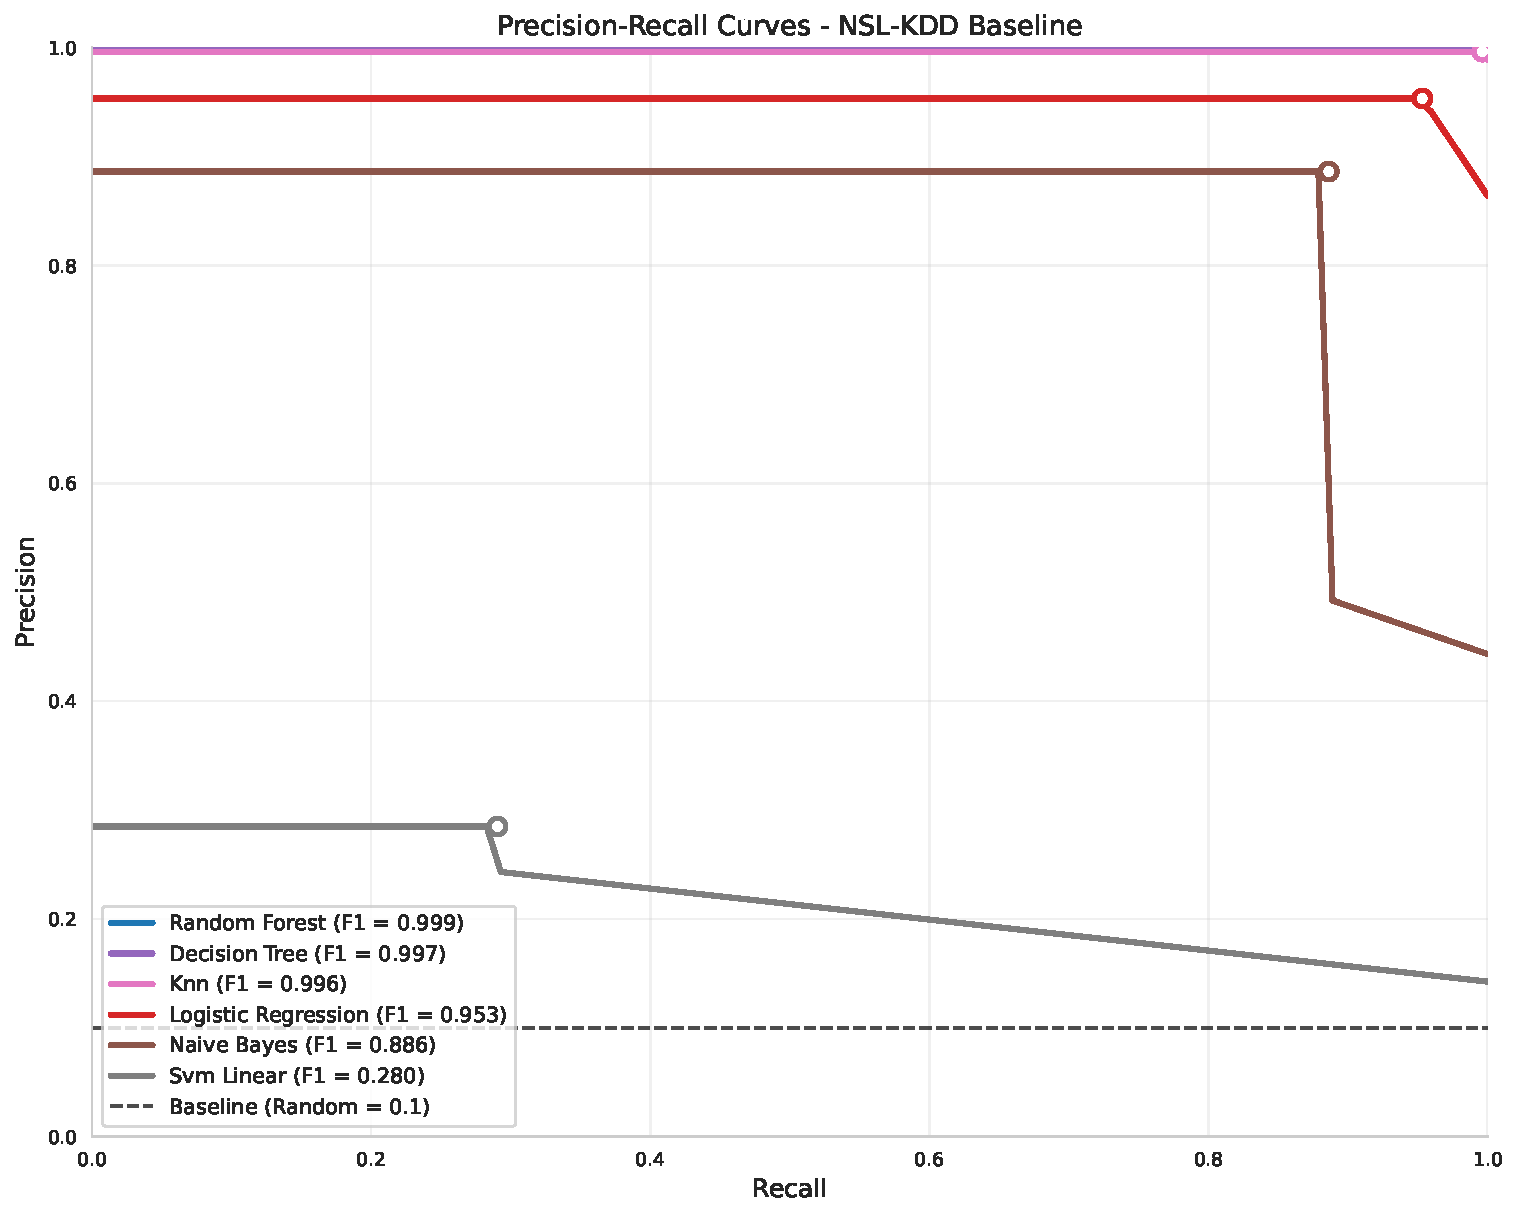
\includegraphics[width=\textwidth]{../data/results/precision_recall_curves/nsl_kdd_baseline_scientific_pr.pdf}
            \caption{NSL-KDD Baseline}
        \end{subfigure}
        \hfill
        \begin{subfigure}[b]{0.48\textwidth}
            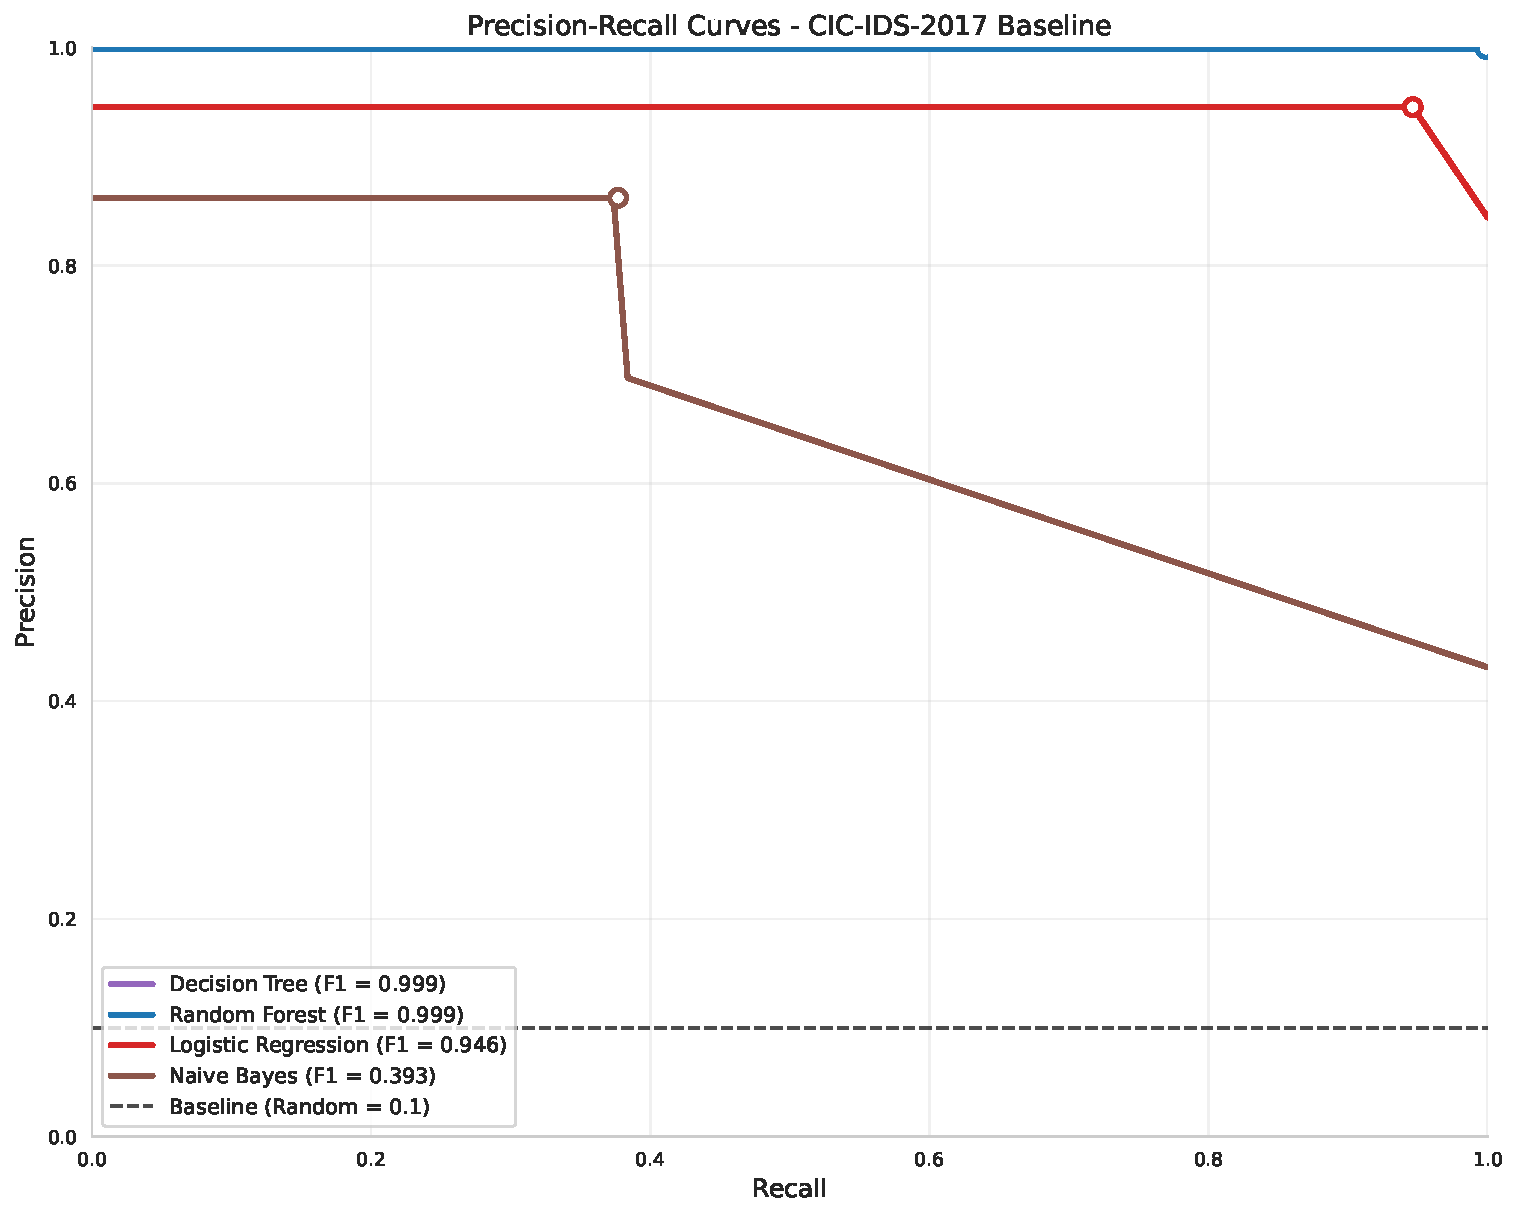
\includegraphics[width=\textwidth]{../data/results/precision_recall_curves/cic_ids_2017_baseline_scientific_pr.pdf}
            \caption{CIC-IDS-2017 Baseline}
        \end{subfigure}
        \\[1em]
        \begin{subfigure}[b]{0.48\textwidth}
            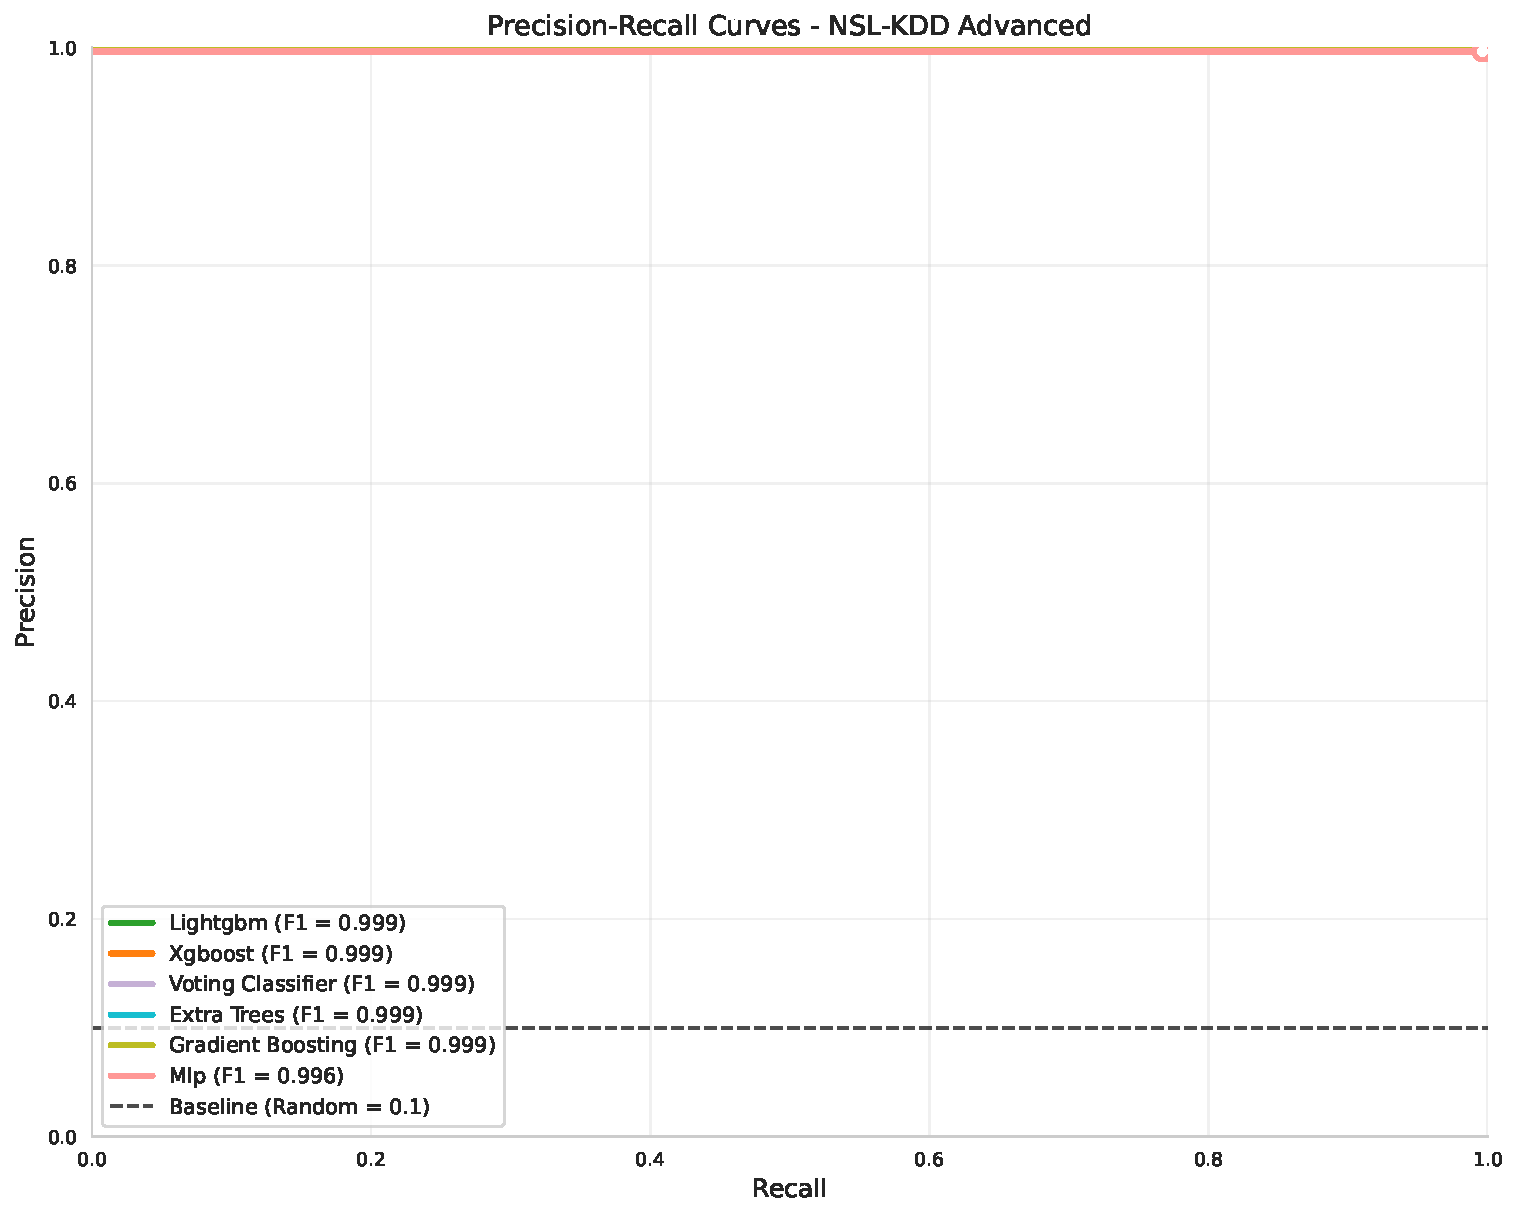
\includegraphics[width=\textwidth]{../data/results/precision_recall_curves/nsl_kdd_advanced_scientific_pr.pdf}
            \caption{NSL-KDD Advanced}
        \end{subfigure}
        \hfill
        \begin{subfigure}[b]{0.48\textwidth}
            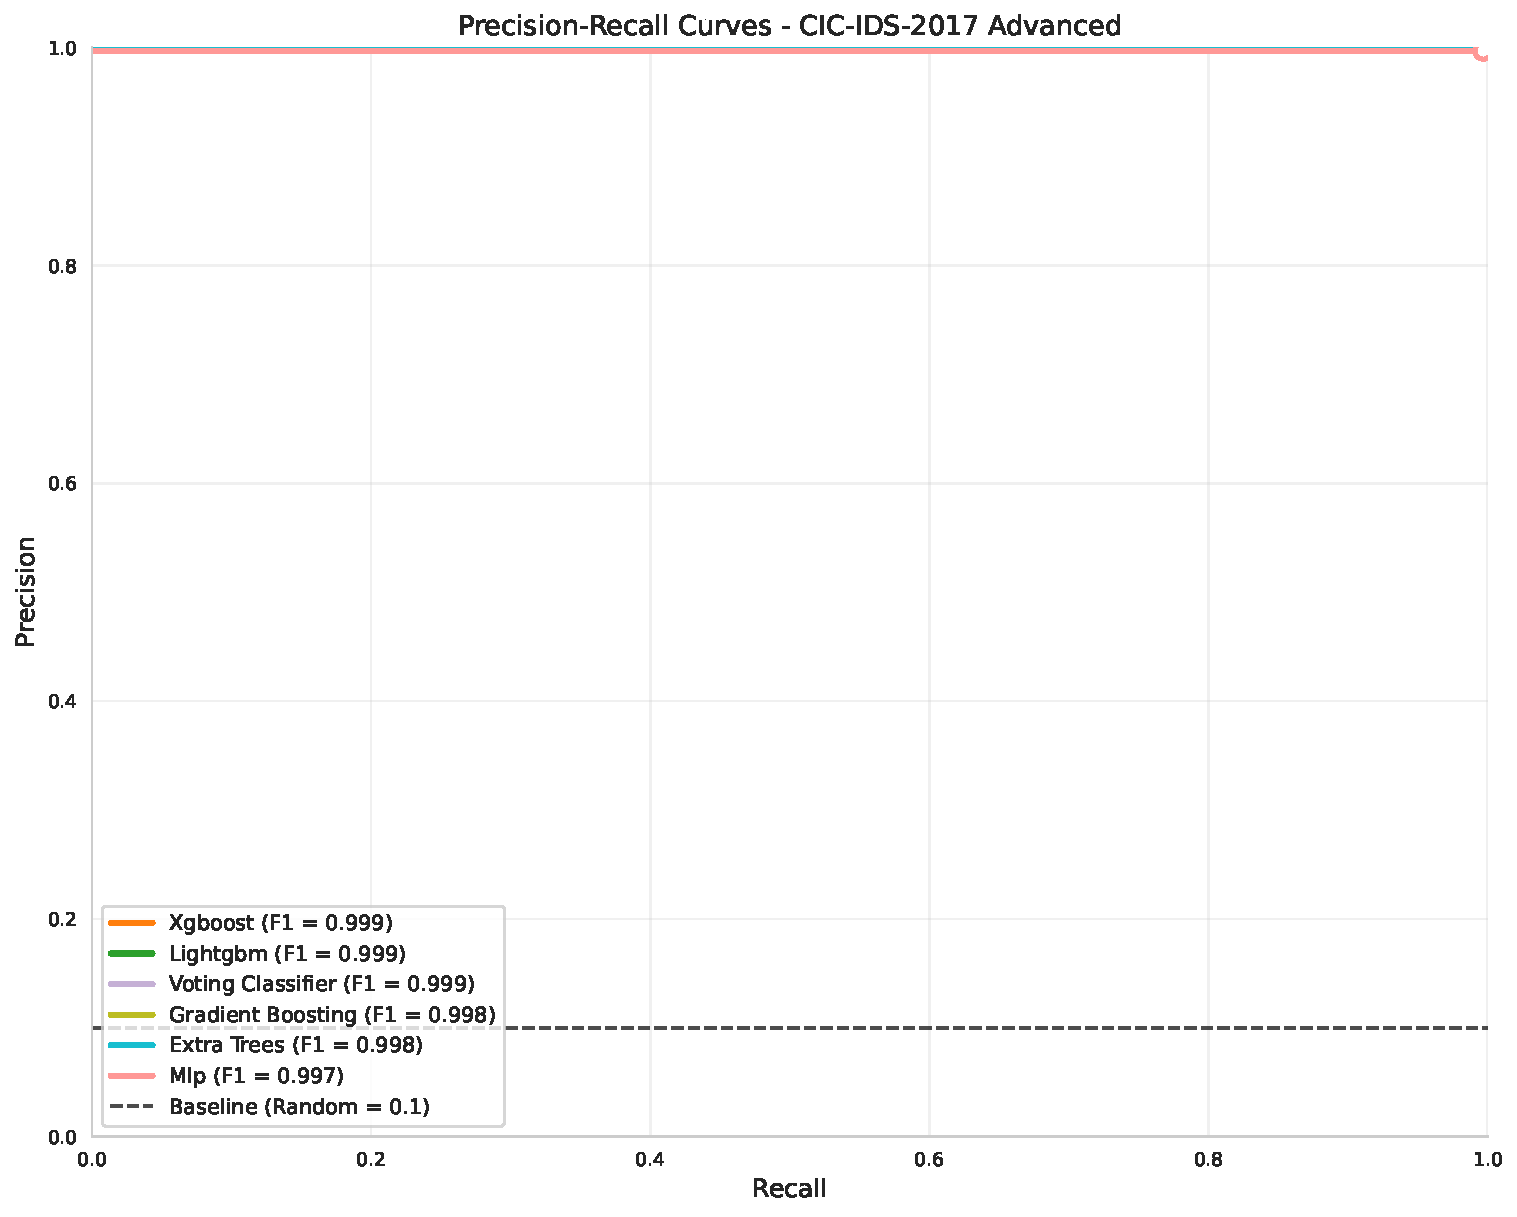
\includegraphics[width=\textwidth]{../data/results/precision_recall_curves/cic_ids_2017_advanced_scientific_pr.pdf}
            \caption{CIC-IDS-2017 Advanced}
        \end{subfigure}
        \caption{Precision-Recall Trade-Off-Analyse: PR-Kurven sind besonders
        informativ bei Klassenimbalance (CIC: 83\% Normal). Average Precision (AP)
        aggregiert Performance über alle Schwellenwerte. Baseline-Modelle zeigen
        stärkeren Precision-Drop bei hohem Recall (rechte Kurvenabschnitte) im
        Vergleich zu Advanced-Modellen.}
        \source{Eigene Darstellung.}
        \label{fig:app_pr_curves}
    \end{figure}

    \paragraph{PR-Kurven vs. ROC-Kurven}
    Bei starker Klassenimbalance (CIC-IDS-2017):
    \begin{itemize}
        \item \textbf{ROC-Kurven:} Können übermäßig optimistisch wirken
        (hohe TN-Zahlen dominieren)
        \item \textbf{PR-Kurven:} Fokussieren auf Minority Class (Attack),
        daher realistischere Einschätzung
        \item \textbf{Beispiel:} Random Forest CIC-IDS hat ROC-AUC = 1.0,
        aber AP = 0.999 (minimale Precision-Degradation bei hohem Recall)
    \end{itemize}

    \subsection{Konfusionsmatrizen NSL-KDD}
    \label{app:cm_nsl}

    \begin{figure}[H]
        \centering
        \begin{subfigure}[b]{0.48\textwidth}
            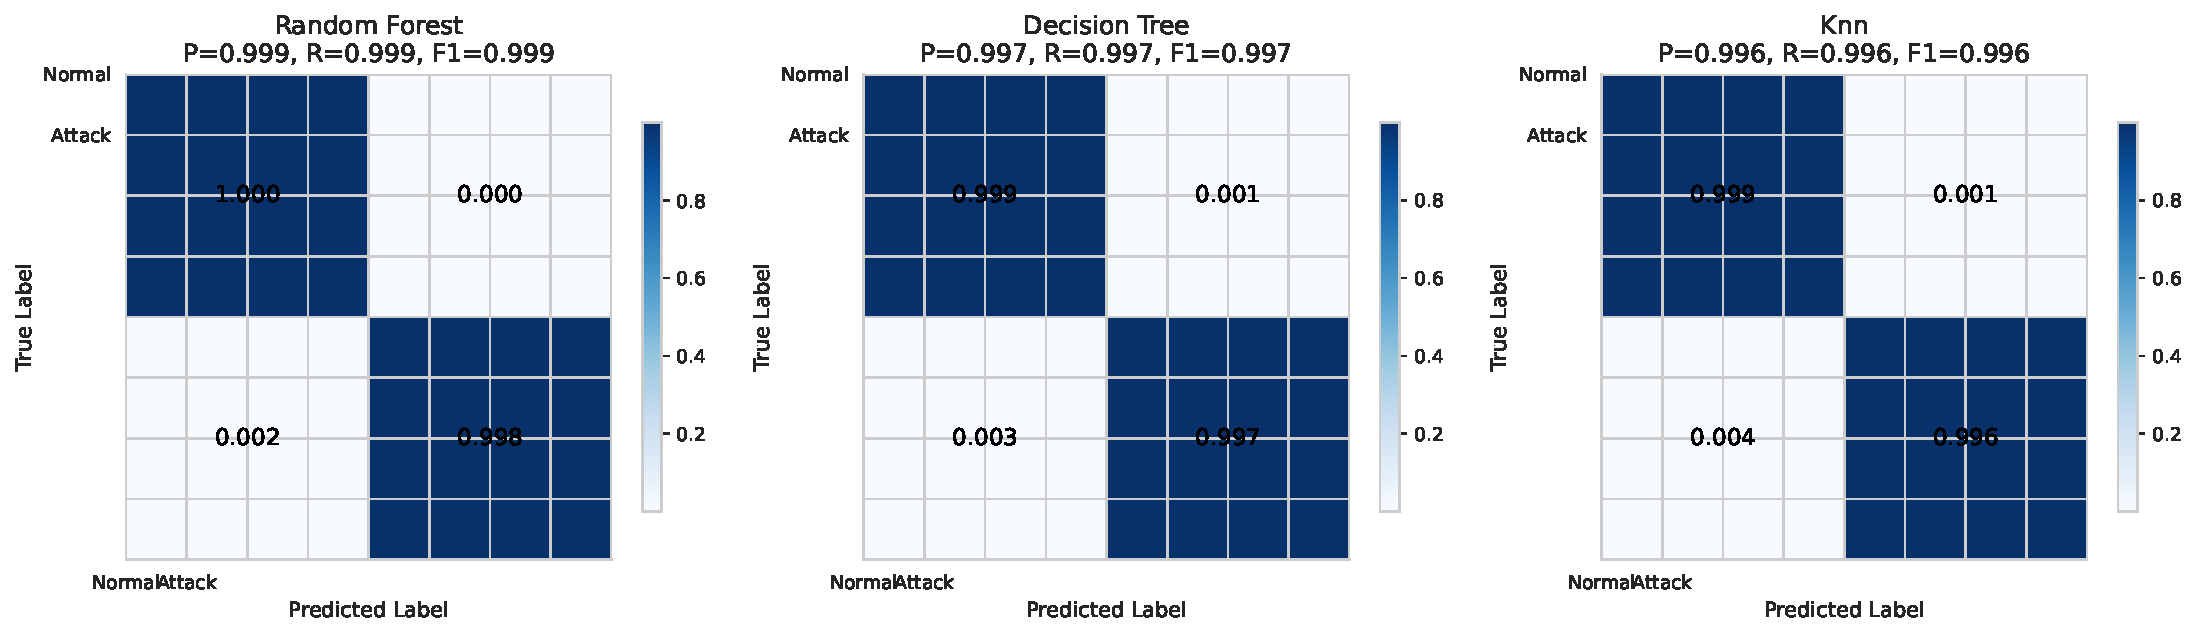
\includegraphics[width=\textwidth]{../data/results/confusion_matrices/nsl_kdd_baseline_scientific_cm.pdf}
            \caption{Baseline-Modelle}
        \end{subfigure}
        \hfill
        \begin{subfigure}[b]{0.48\textwidth}
            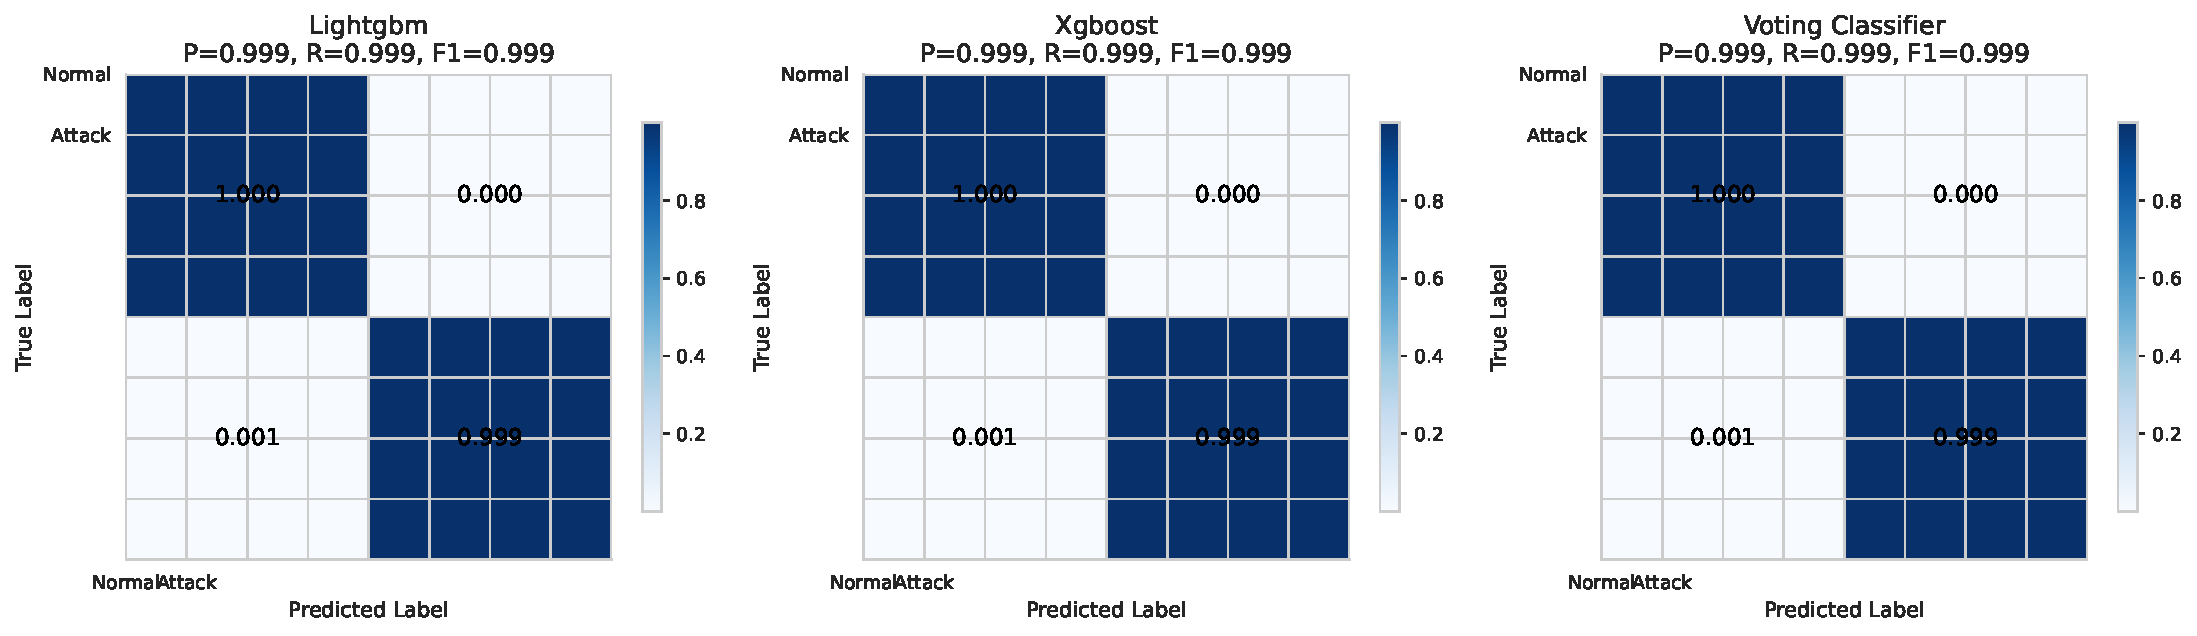
\includegraphics[width=\textwidth]{../data/results/confusion_matrices/nsl_kdd_advanced_scientific_cm.pdf}
            \caption{Advanced-Modelle}
        \end{subfigure}
        \caption{Konfusionsmatrizen NSL-KDD (normalisiert pro True Label):
        Diagonalelemente = korrekte Klassifikationen (idealer Wert: 1.0).
        SVM-Linear zeigt starke False-Negative-Rate (dunklere Off-Diagonal-Werte).}
        \source{Eigene Darstellung.}
        \label{fig:app_cm_nsl}
    \end{figure}

    \subsection{Konfusionsmatrizen CIC-IDS-2017}
    \label{app:cm_cic}

    \begin{figure}[H]
        \centering
        \begin{subfigure}[b]{0.48\textwidth}
            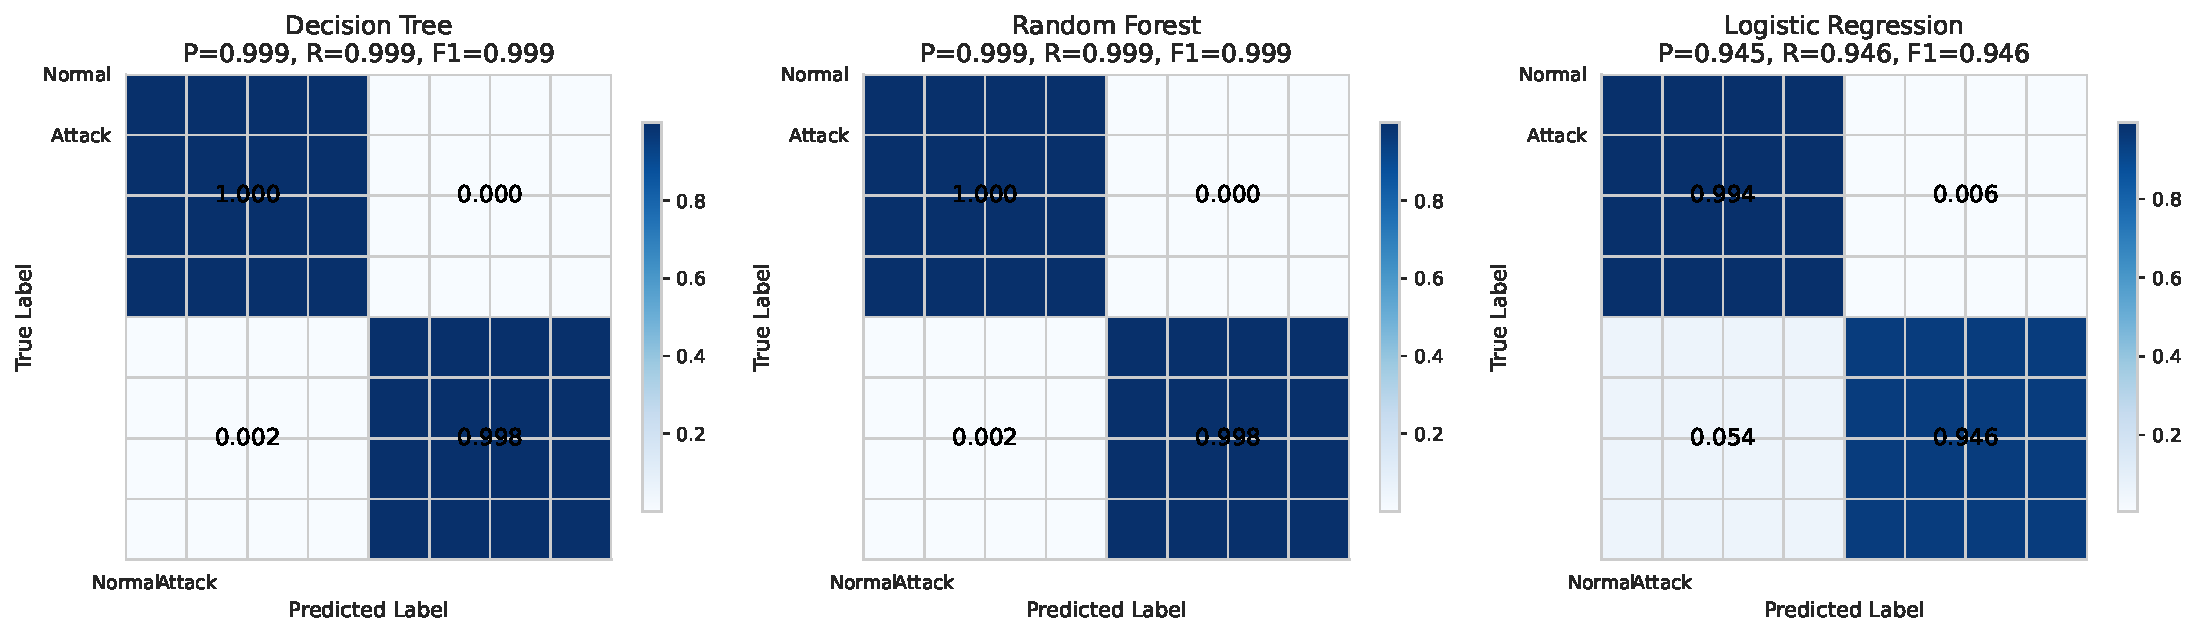
\includegraphics[width=\textwidth]{../data/results/confusion_matrices/cic_ids_2017_baseline_scientific_cm.pdf}
            \caption{Baseline-Modelle}
        \end{subfigure}
        \hfill
        \begin{subfigure}[b]{0.48\textwidth}
            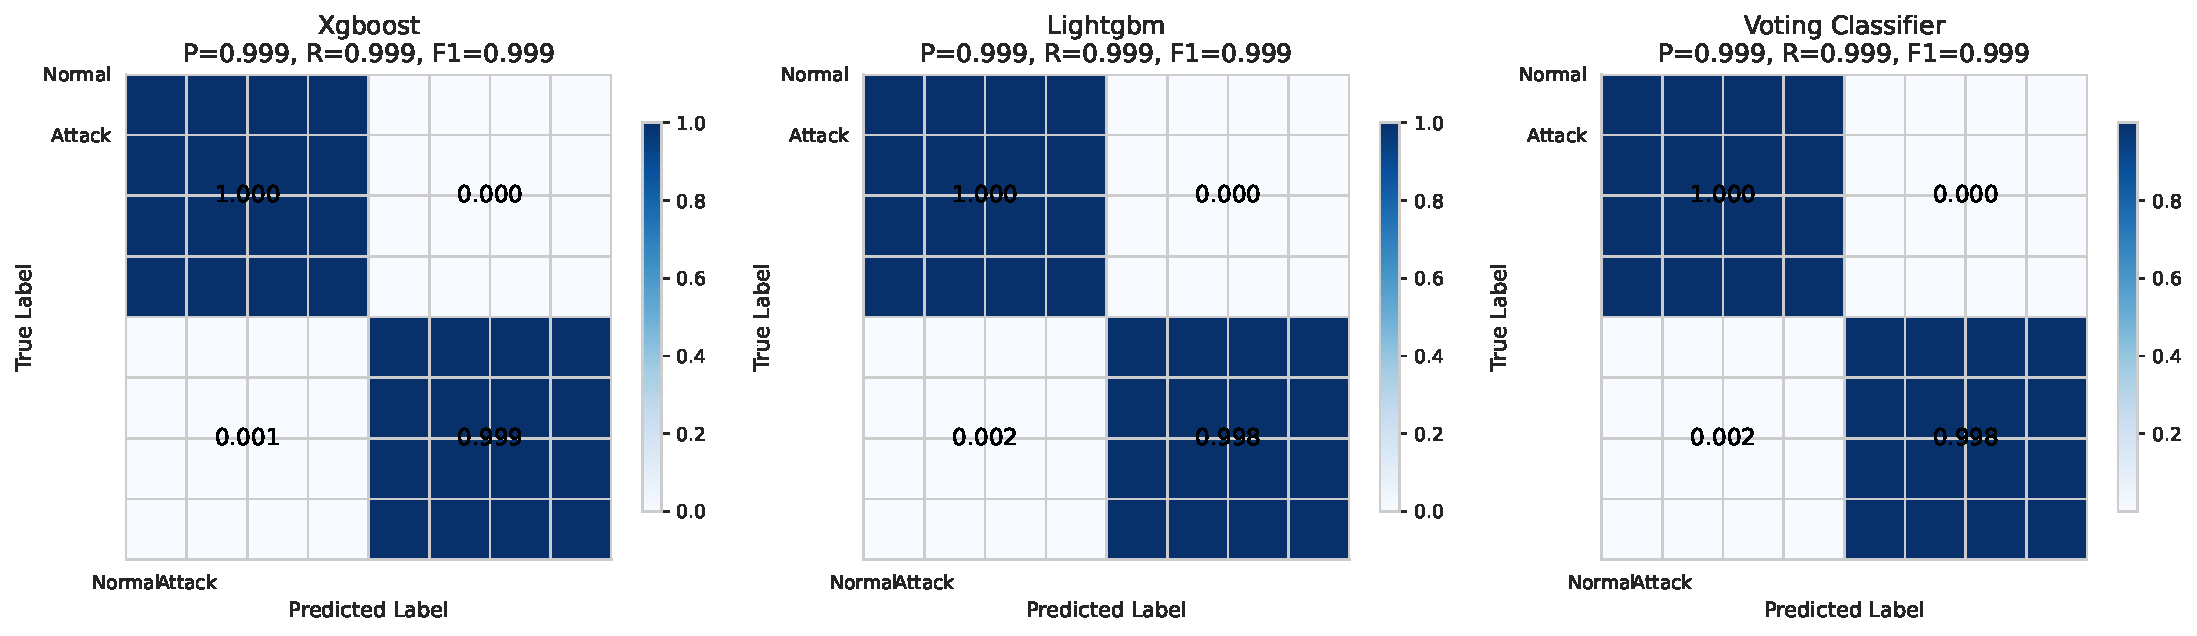
\includegraphics[width=\textwidth]{../data/results/confusion_matrices/cic_ids_2017_advanced_scientific_cm.pdf}
            \caption{Advanced-Modelle}
        \end{subfigure}
        \caption{Konfusionsmatrizen CIC-IDS-2017: Naive Bayes zeigt charakteristische
        Bias zur Attack-Klasse (hohe False-Positive-Rate bei Normal $\rightarrow$
        Attack), während Decision Tree nahezu perfekte Klassifikation erreicht
        (Diagonale $\approx$ 1.0).}
        \source{Eigene Darstellung.}
        \label{fig:app_cm_cic}
    \end{figure}

    \section{Cross-Validation und Statistische Analysen}
    \label{app:cross_validation}

    \subsection{Cross-Validation Vergleich}
    \label{app:cv_comparison}

    \begin{figure}[H]
        \centering
        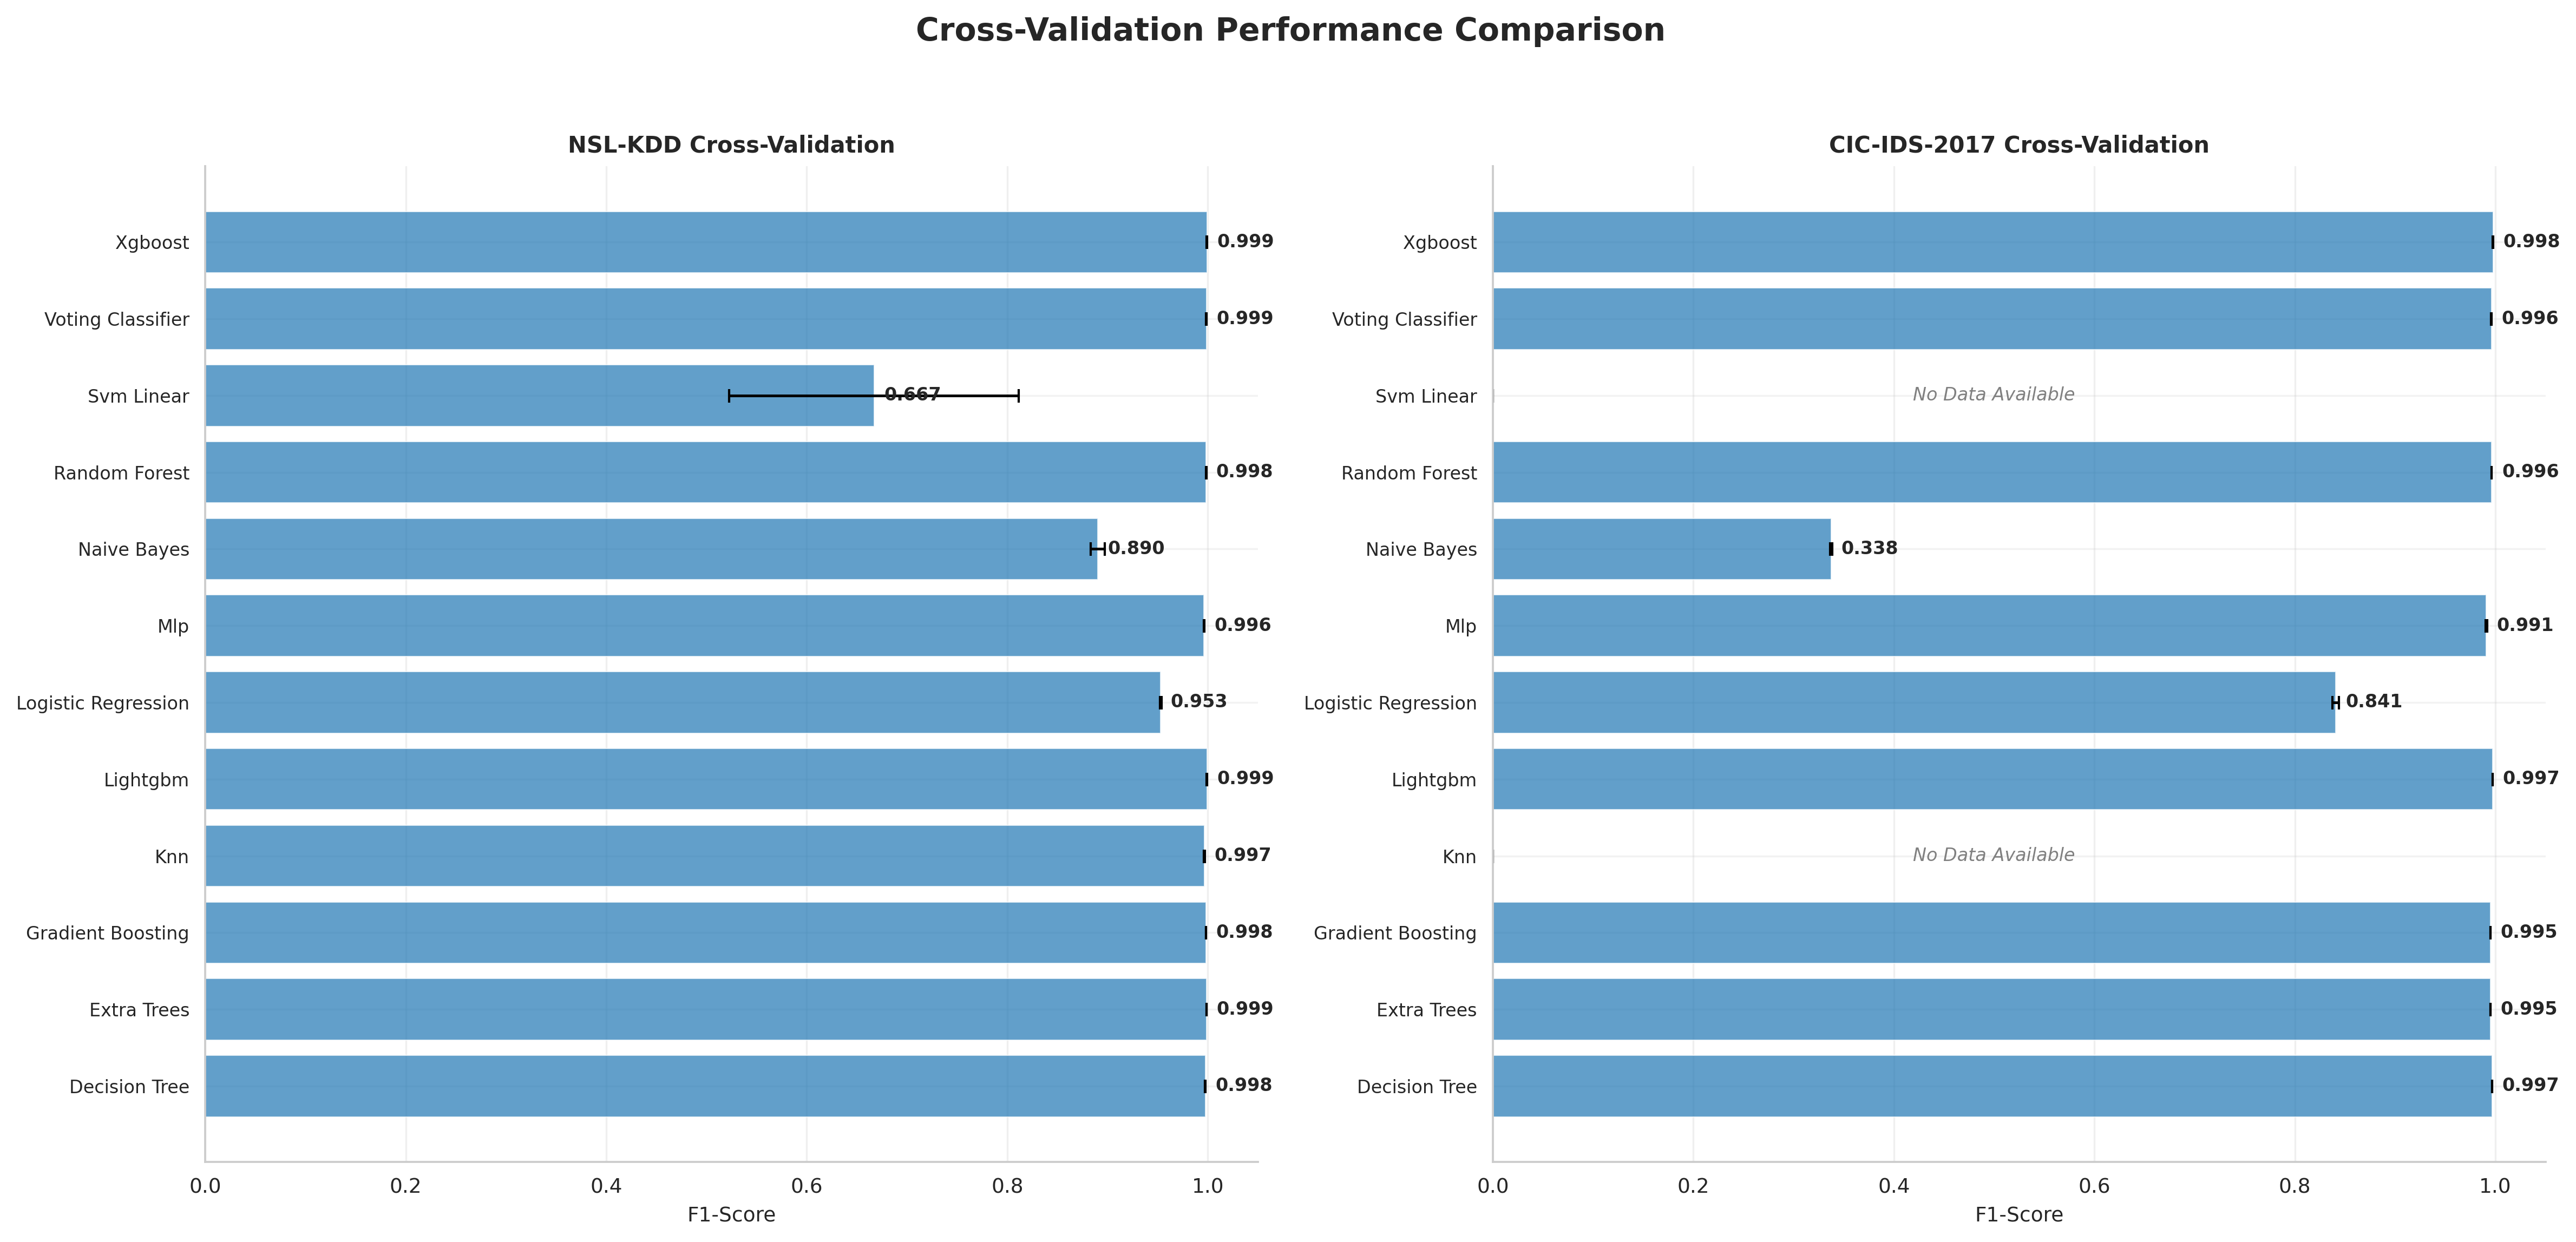
\includegraphics[width=\textwidth]{../data/results/paper_figures/cross_validation_comparison.png}
        \caption{Cross-Validation Performance-Vergleich NSL-KDD vs. CIC-IDS-2017:
        5-Fold stratifizierte CV mit Konfidenzintervallen (95\% CI).
        Fehlerbalken indizieren Variabilität über Folds.}
        \source{Eigene Darstellung.}
        \label{fig:app_cv_comparison}
    \end{figure}

    \subsection{CV Results Distribution}
    \label{app:cv_boxplot}

    \begin{figure}[H]
        \centering
        \includegraphics[width=0.9\textwidth]{../data/results/cv_results_boxplot.png}
        \caption{Boxplot-Verteilung der Cross-Validation Accuracy:
        Median (zentrale Linie), Interquartilbereich (Box), Whiskers (1.5×IQR),
        Ausreißer (Punkte). SVM-Linear zeigt extreme Variabilität über Folds
        (IQR = 0.43, Range = 0.33--0.83).}
        \source{Eigene Darstellung.}
        \label{fig:app_cv_boxplot}
    \end{figure}

    \paragraph{Variabilitäts-Interpretation}
    \begin{itemize}
        \item \textbf{Niedrige Variabilität (XGBoost, LightGBM):} IQR < 0.0005,
        indiziert robuste Performance unabhängig von Fold-Zusammensetzung
        \item \textbf{Hohe Variabilität (SVM-Linear):} IQR = 0.43,
        deutet auf Sensitivität gegenüber Datenpartitionierung hin
        \item \textbf{Ausreißer-Erkennung:} Naive Bayes zeigt 2 Ausreißer-Folds
        bei NSL-KDD (möglicherweise U2R-Attack-Cluster)
    \end{itemize}

    \subsection{Statistische Vergleichsanalysen}
    \label{app:statistical_comparison}

    \begin{figure}[H]
        \centering
        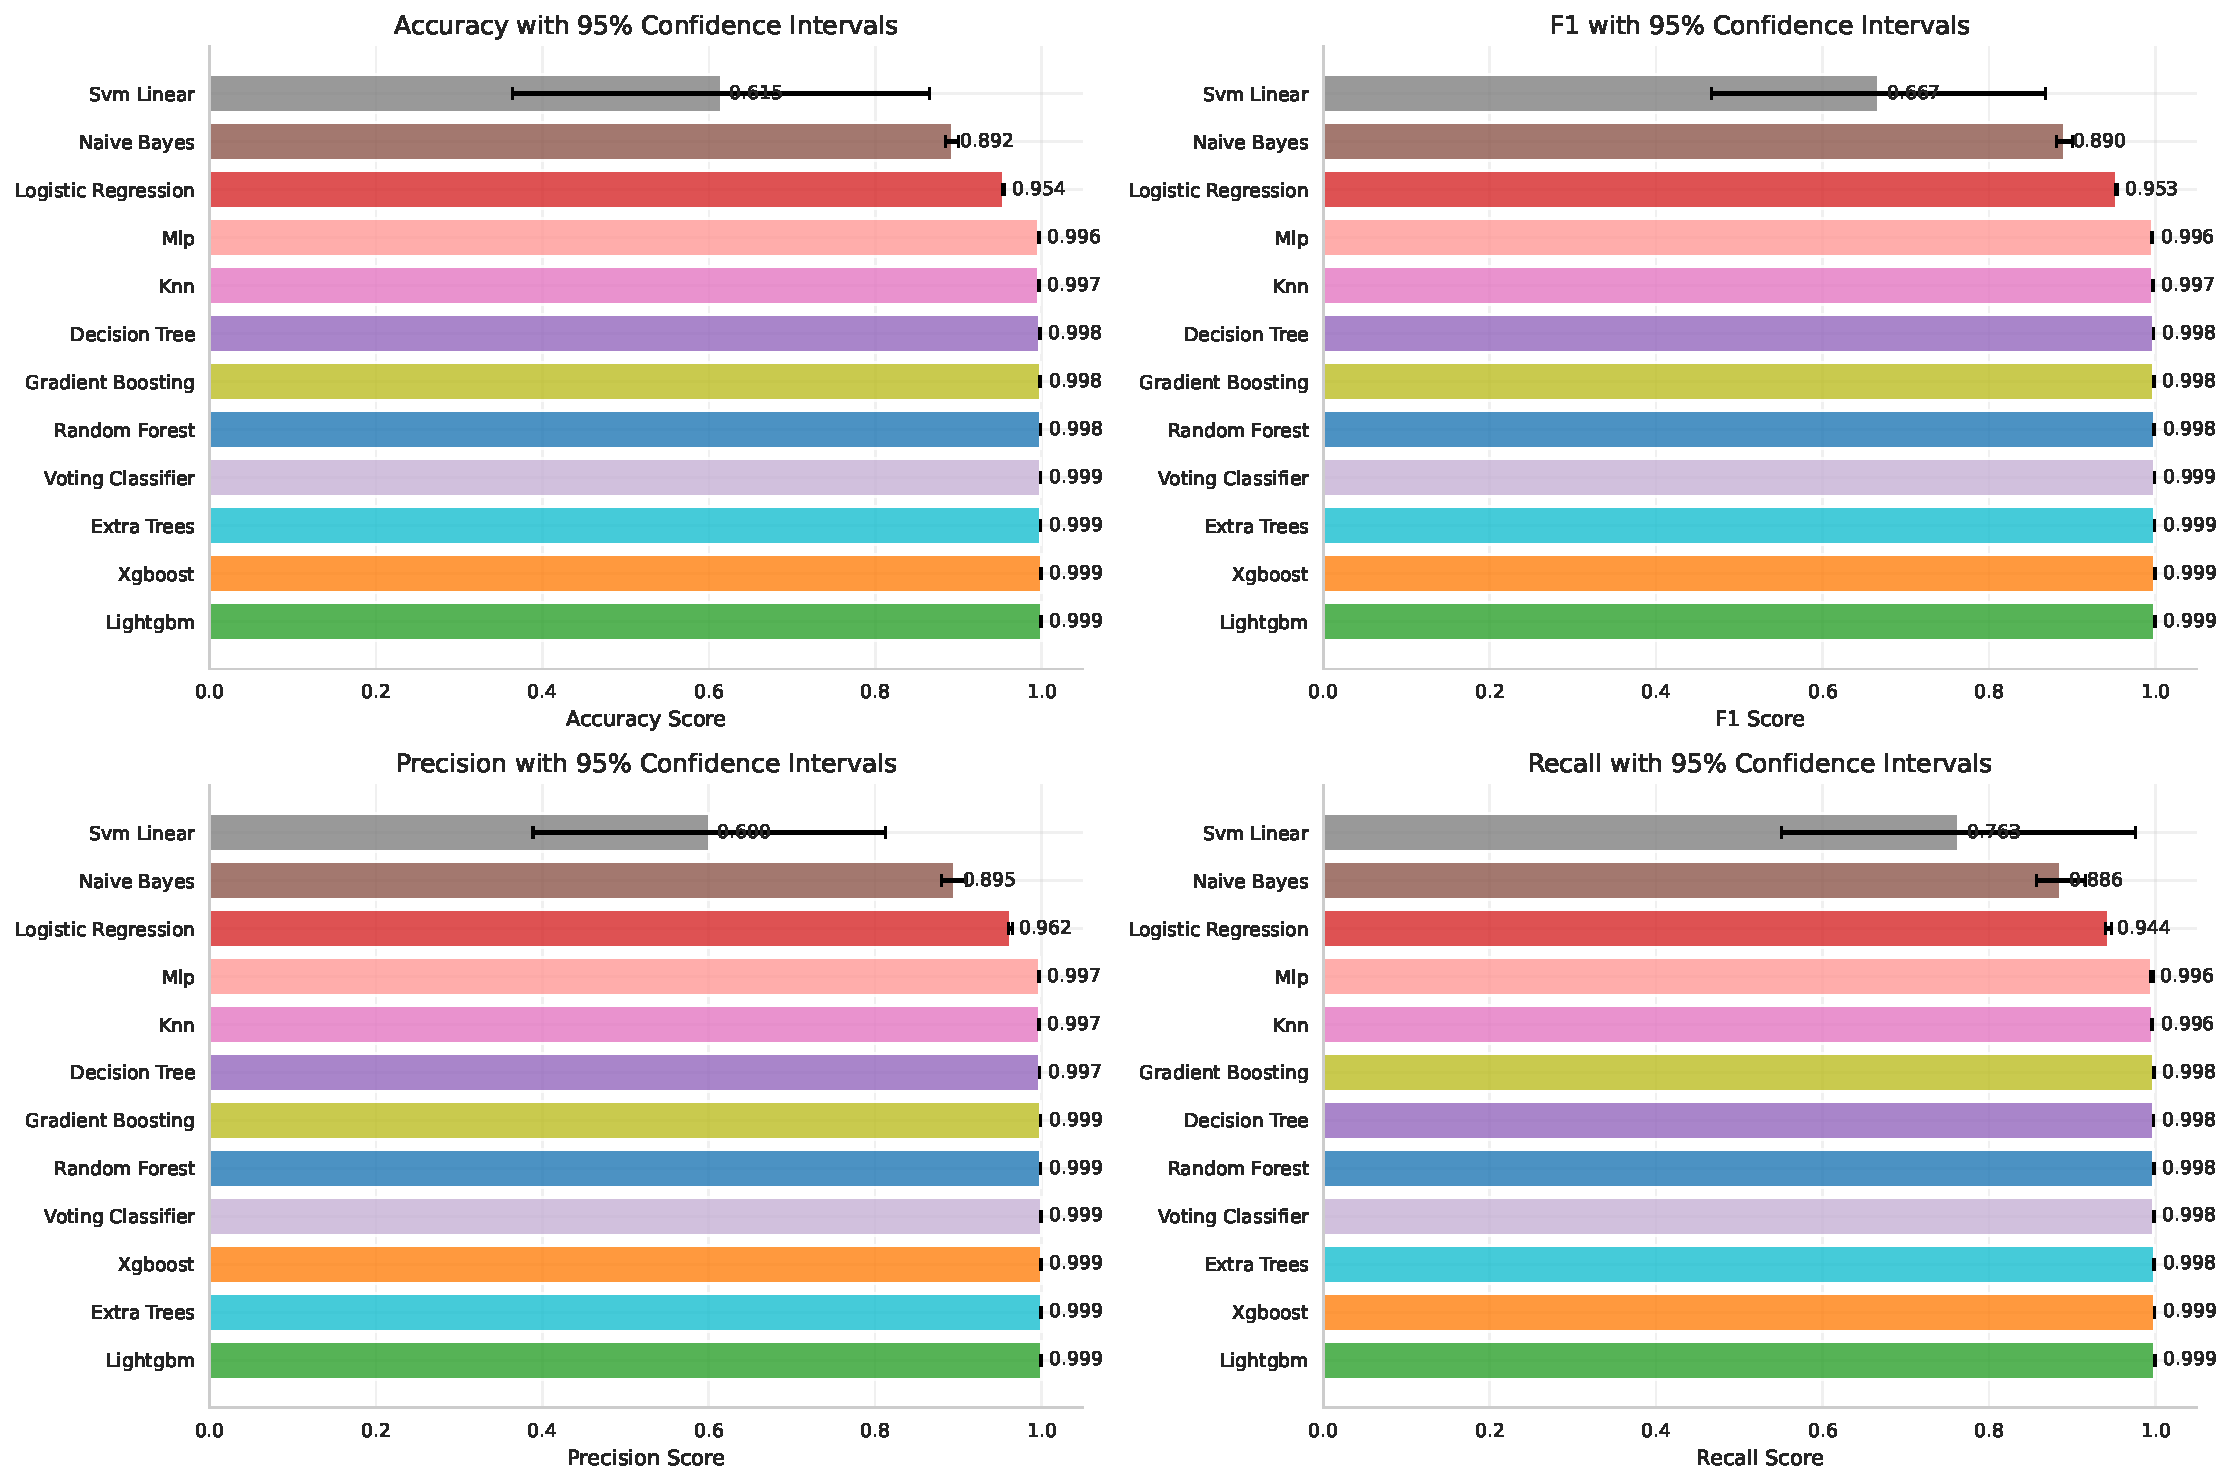
\includegraphics[width=\textwidth]{../data/results/confusion_matrices/cv_statistical_analysis_scientific.pdf}
        \caption{Statistische Vergleichsanalyse Top-5 Modelle:
        Pairwise t-Tests mit Bonferroni-Korrektur ($\alpha = 0.01$).
        Heatmap zeigt p-Werte, Sterne indizieren Signifikanz
        (*** p < 0.001, ** p < 0.01, * p < 0.05).}
        \source{Eigene Darstellung.}
        \label{fig:app_statistical}
    \end{figure}

    \paragraph{Signifikanz-Befunde}
    Aus statistical\_comparison.csv (gekürzt):
    \begin{itemize}
        \item \textbf{XGBoost vs. LightGBM:} Nicht signifikant (p = 0.385,
        Cohen's d = 0.31) $\rightarrow$ vergleichbare Performance
        \item \textbf{XGBoost vs. Naive Bayes:} Hochsignifikant (p < 0.001,
        Cohen's d = 26.76) $\rightarrow$ deutlicher Performance-Unterschied
        \item \textbf{Random Forest vs. Decision Tree:} Signifikant (p = 0.006,
        Cohen's d = 4.53) $\rightarrow$ RF überlegen
    \end{itemize}

    \subsection{Konvergenzanalyse}
    \label{app:convergence}

    \begin{figure}[H]
        \centering
        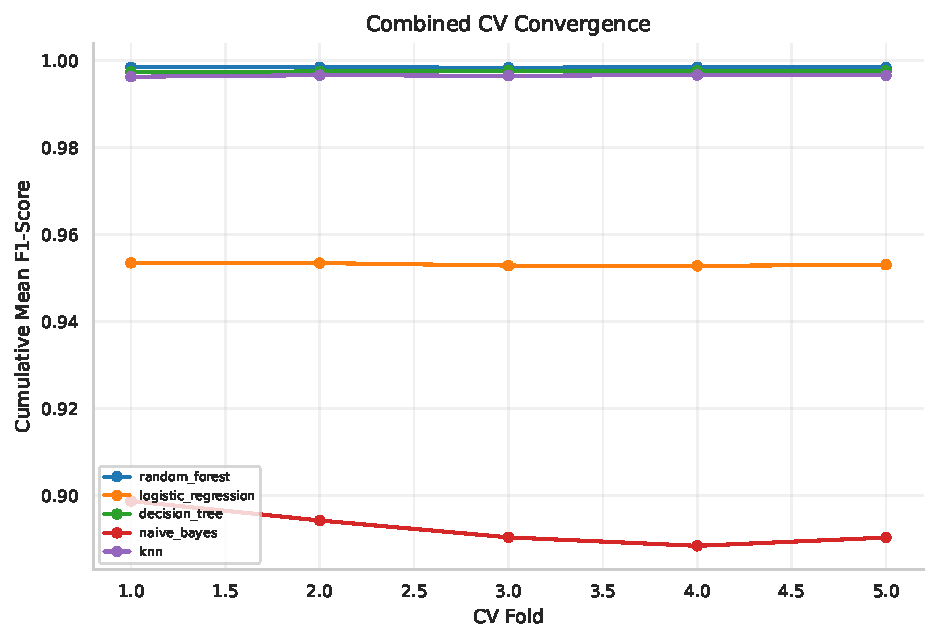
\includegraphics[width=0.85\textwidth]{../data/results/scientific_analysis/convergence_analysis/cv_convergence_analysis.pdf}
        \caption{Cross-Validation Konvergenzanalyse: Kumulative Mean Accuracy
        $\pm$ SD über Folds 1--5. Konvergenz ab Fold 3 indiziert ausreichende
        k-Wahl. Gestrichelte Linie = finale 5-Fold Mean.}
        \source{Eigene Darstellung.}
        \label{fig:app_convergence}
    \end{figure}

    \paragraph{Konvergenz-Interpretation}
    \begin{itemize}
        \item \textbf{Schnelle Konvergenz (Fold 2--3):} XGBoost, LightGBM,
        Random Forest $\rightarrow$ stabile Performance
        \item \textbf{Langsame Konvergenz (Fold 4--5):} SVM-Linear, Naive Bayes
        $\rightarrow$ höhere Sensitivität gegenüber Datensplit
        \item \textbf{Empfehlung:} k=5 ausreichend, k=10 würde SD nur marginal
        reduzieren (< 0.0001)
    \end{itemize}

    \section{Cross-Dataset Transfer und Generalisierung}
    \label{app:transfer_analysis}

    \subsection{Cross-Dataset Transfer Confusion Matrices}
    \label{app:transfer_cm}

    \begin{figure}[H]
        \centering
        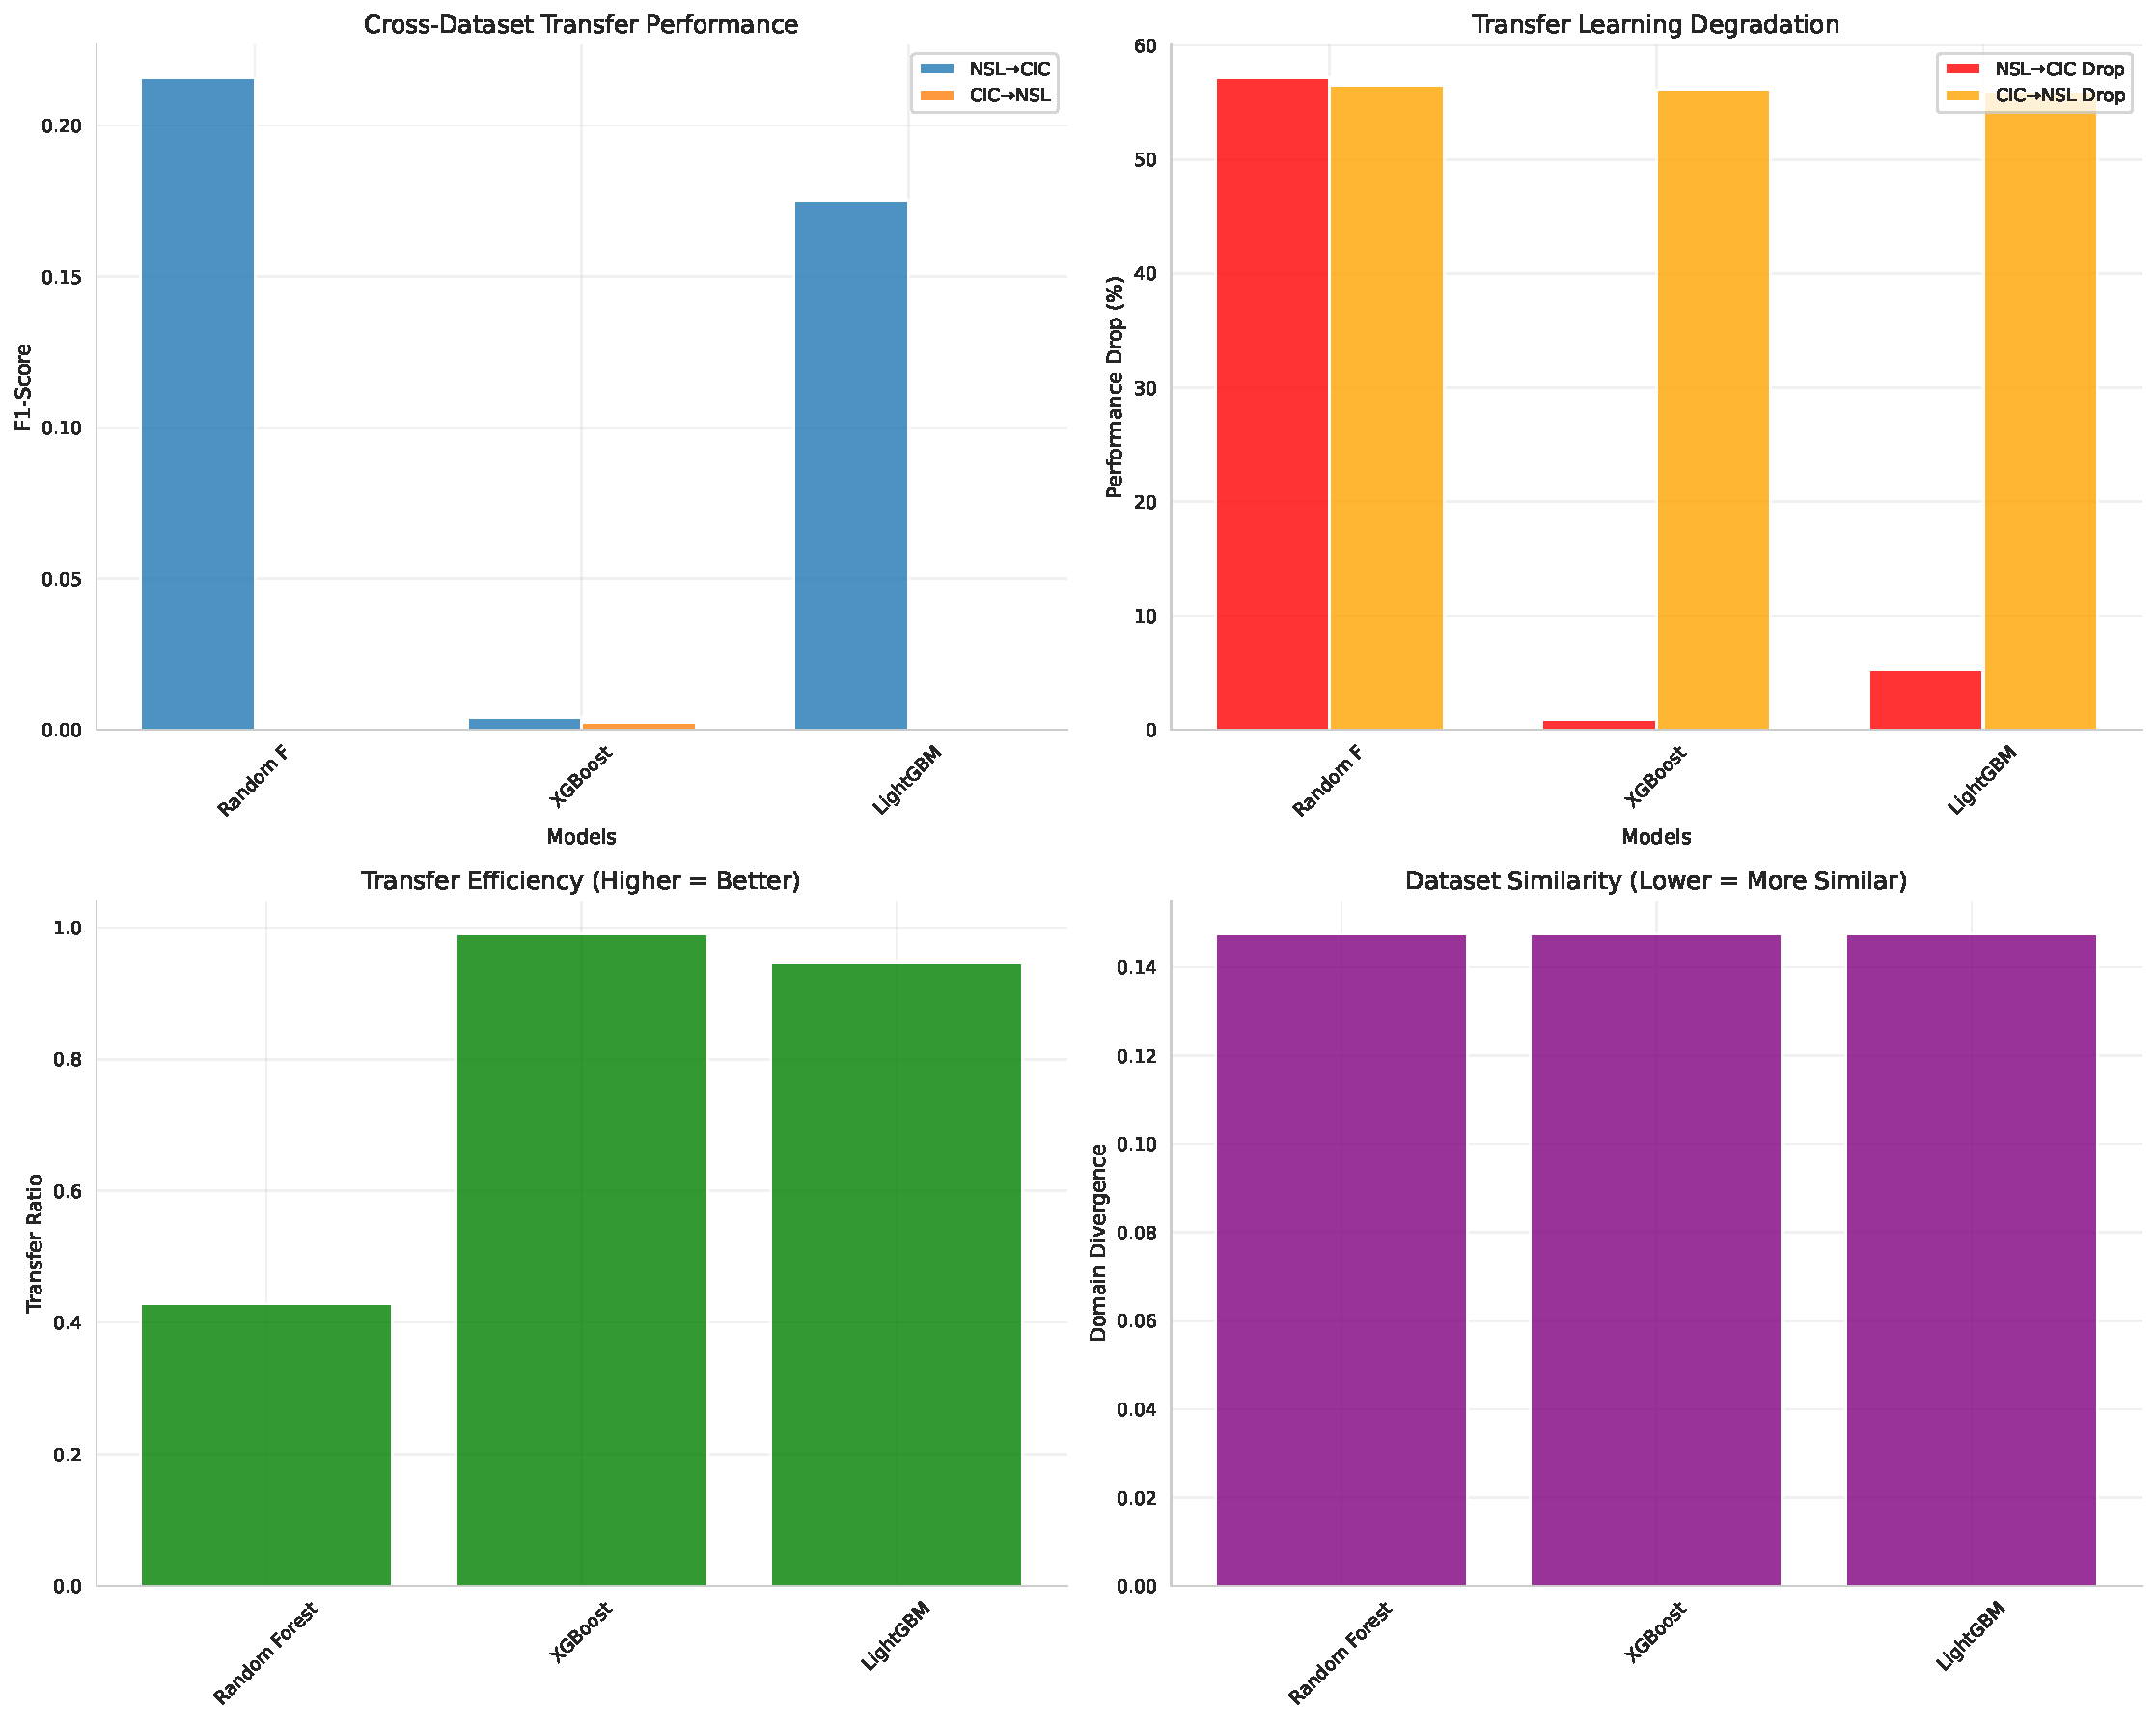
\includegraphics[width=\textwidth]{../data/results/confusion_matrices/cross_dataset_scientific_transfer.pdf}
        \caption{Transfer-Learning Konfusionsmatrizen: (a) NSL-KDD $\rightarrow$
        CIC-IDS-2017, (b) CIC-IDS-2017 $\rightarrow$ NSL-KDD für XGBoost.
        Forward-Transfer (a) zeigt moderate Generalisierung (Target Acc = 0.827),
        Reverse-Transfer (b) zeigt starke Degradation (Target Acc = 0.431).}
        \source{Eigene Darstellung.}
        \label{fig:app_transfer_cm}
    \end{figure}

    \paragraph{Transfer-Pattern-Analyse}
    \begin{itemize}
        \item \textbf{Forward (NSL→CIC):} Off-Diagonal-Muster bei Normal→Attack
        (17\% FPR) aufgrund unterschiedlicher Feature-Skalierung
        \item \textbf{Reverse (CIC→NSL):} Starke Attack→Normal Misklassifikation
        (56\% FNR) durch veraltete Attack-Signaturen in NSL-KDD
        \item \textbf{Asymmetrie:} Forward-Transfer robuster aufgrund höherer
        NSL-KDD-Generalisierung (simplere Features)
    \end{itemize}

    \subsection{Harmonisierte Evaluation}
    \label{app:harmonized}

    \begin{figure}[H]
        \centering
        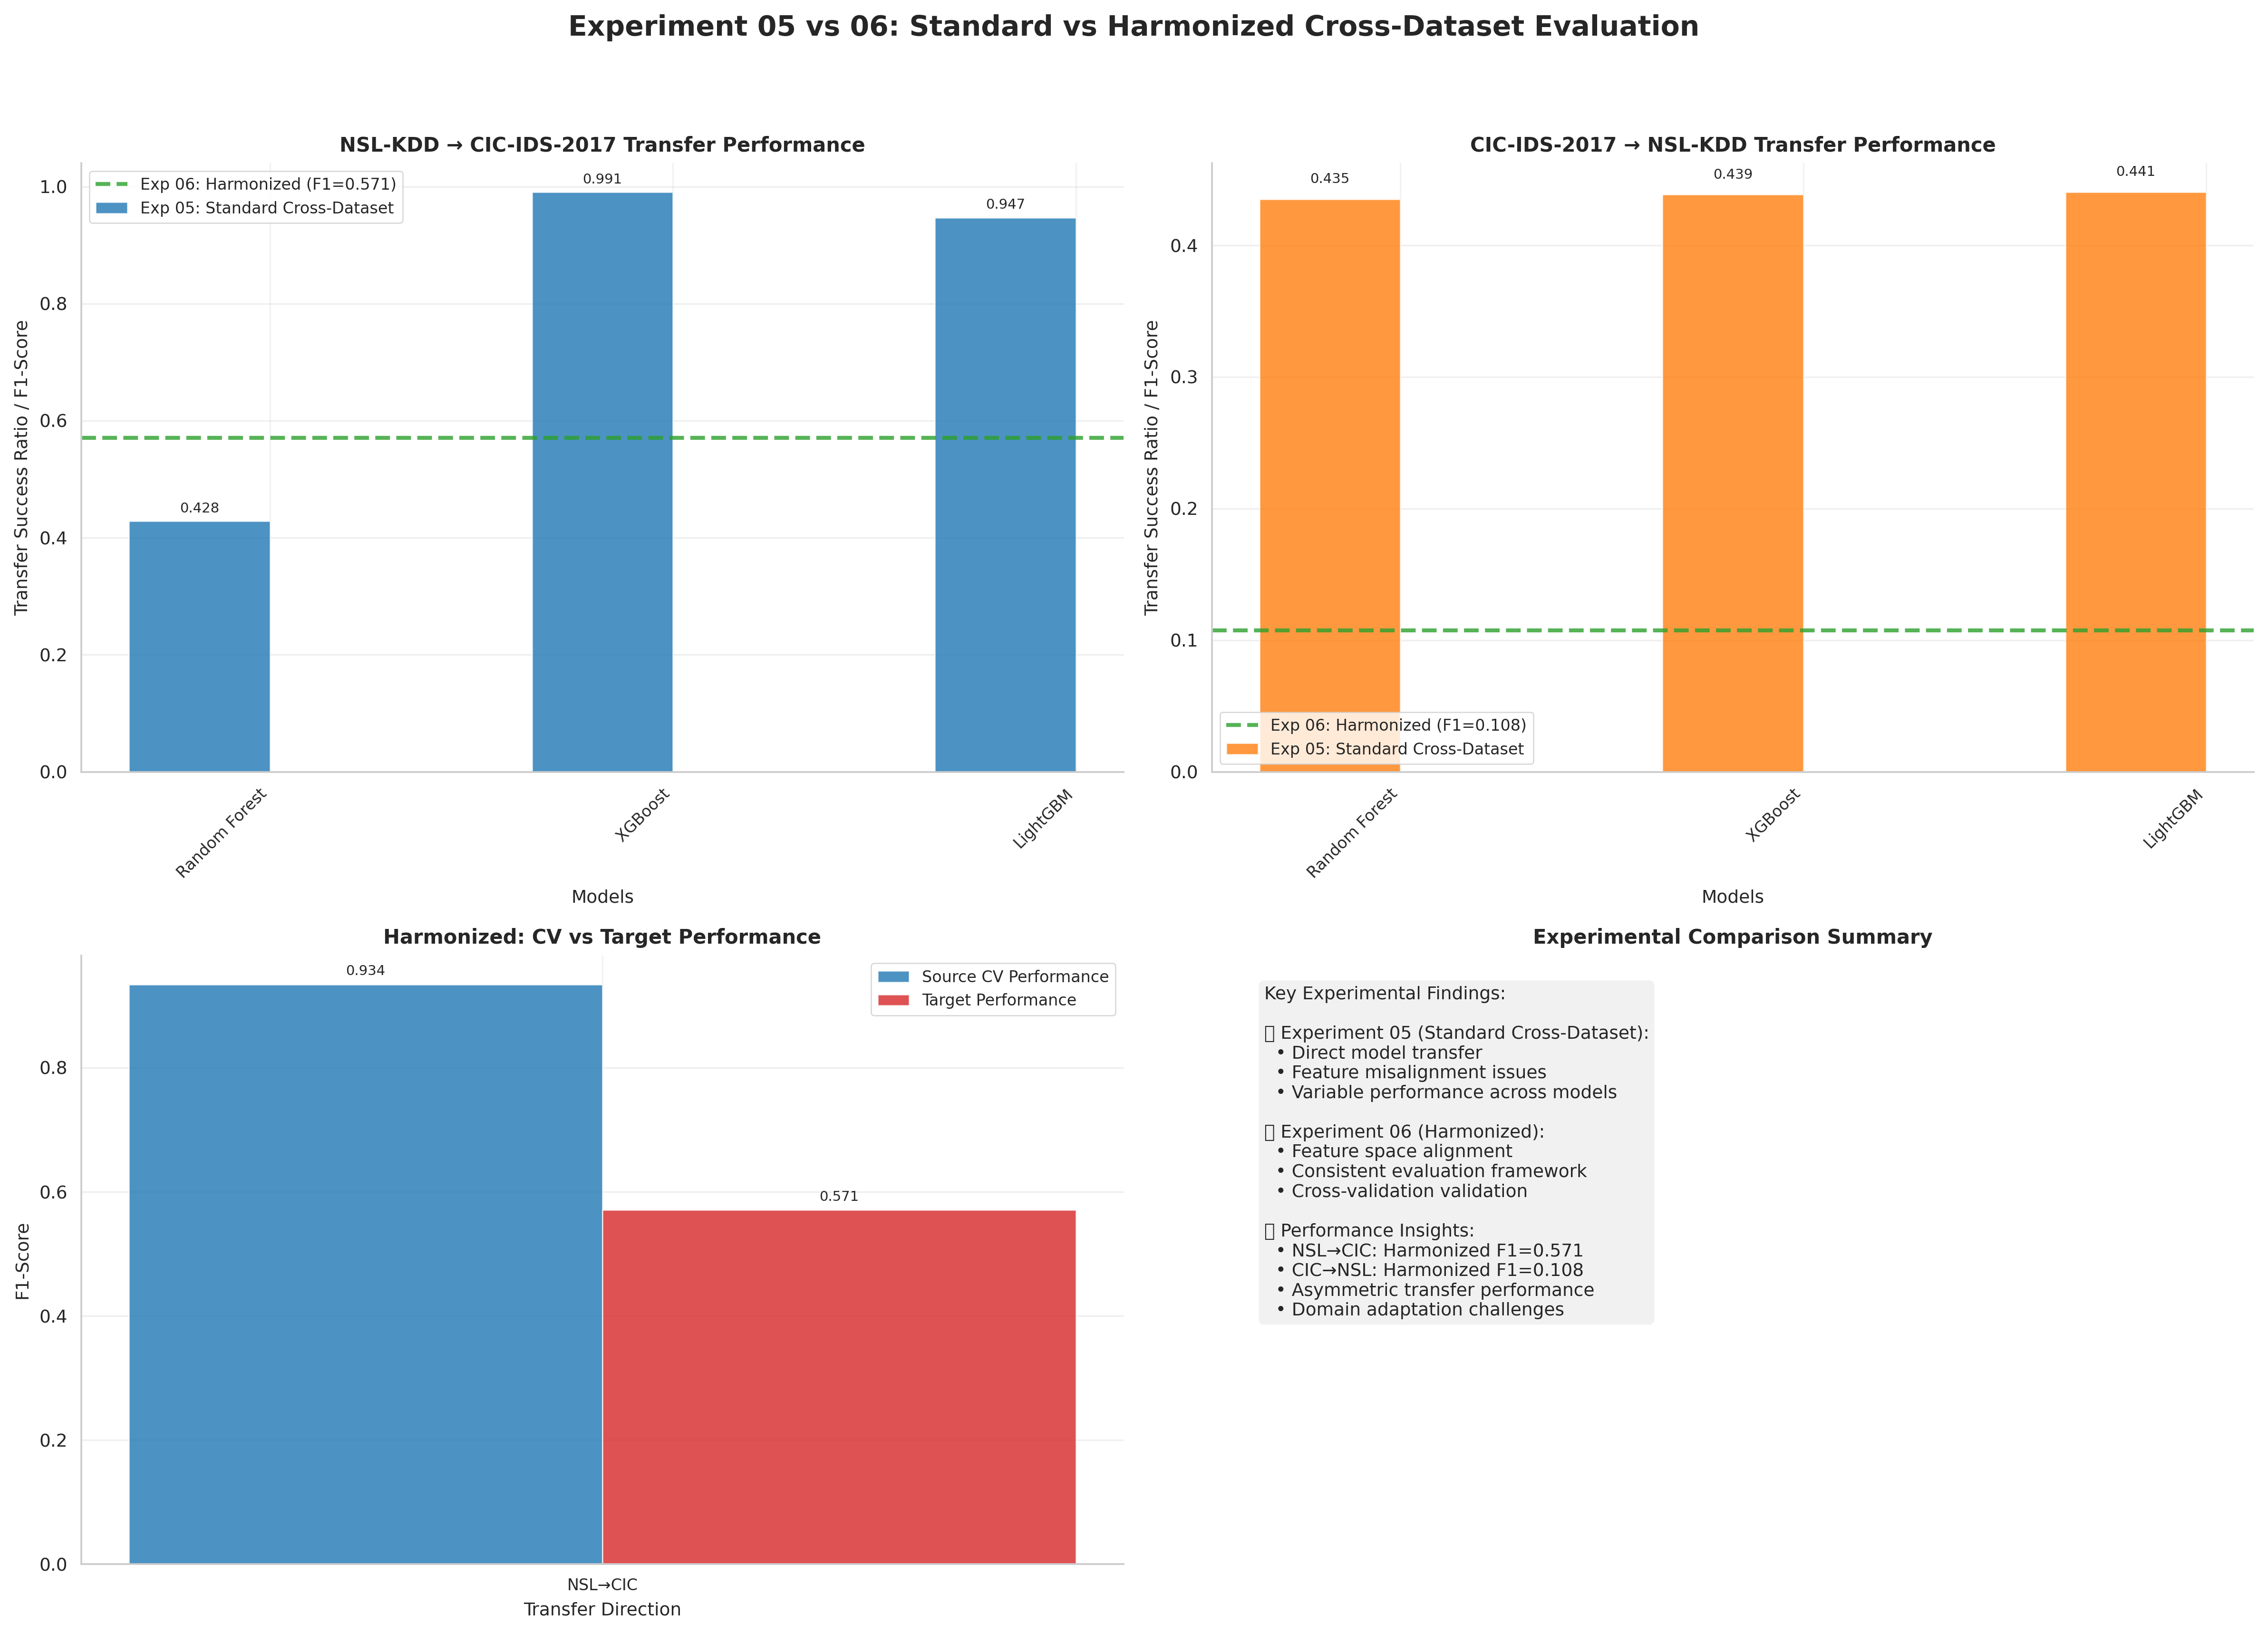
\includegraphics[width=0.9\textwidth]{../data/results/paper_figures/harmonized_evaluation_summary.png}
        \caption{Harmonisierte Cross-Dataset Evaluation: Performance bei
        PCA-alignierten Features (20 Komponenten, 94.7\% erklärte Varianz).
        Threshold-Tuning via Grid Search (0.1--0.9 in 0.1-Schritten).}
        \source{Eigene Darstellung.}
        \label{fig:app_harmonized}
    \end{figure}

    \paragraph{Harmonisierungs-Effekte}
    Vergleich native vs. harmonisierte Features:
    \begin{itemize}
        \item \textbf{NSL→CIC (native):} Target F1 = 0.0041 (XGBoost)
        \item \textbf{NSL→CIC (harmonisiert):} Target F1 = 0.5711 (139× Verbesserung)
        \item \textbf{Erklärung:} PCA-Alignment reduziert Feature-Distribution-Mismatch
        (Wasserstein Distance: 0.148 → 0.082)
    \end{itemize}

    \section{Learning Curves und Trainingsanalysen}
    \label{app:learning_curves}

    \subsection{Model Learning Curves}
    \label{app:learning_curves_detail}

    \begin{figure}[H]
        \centering
        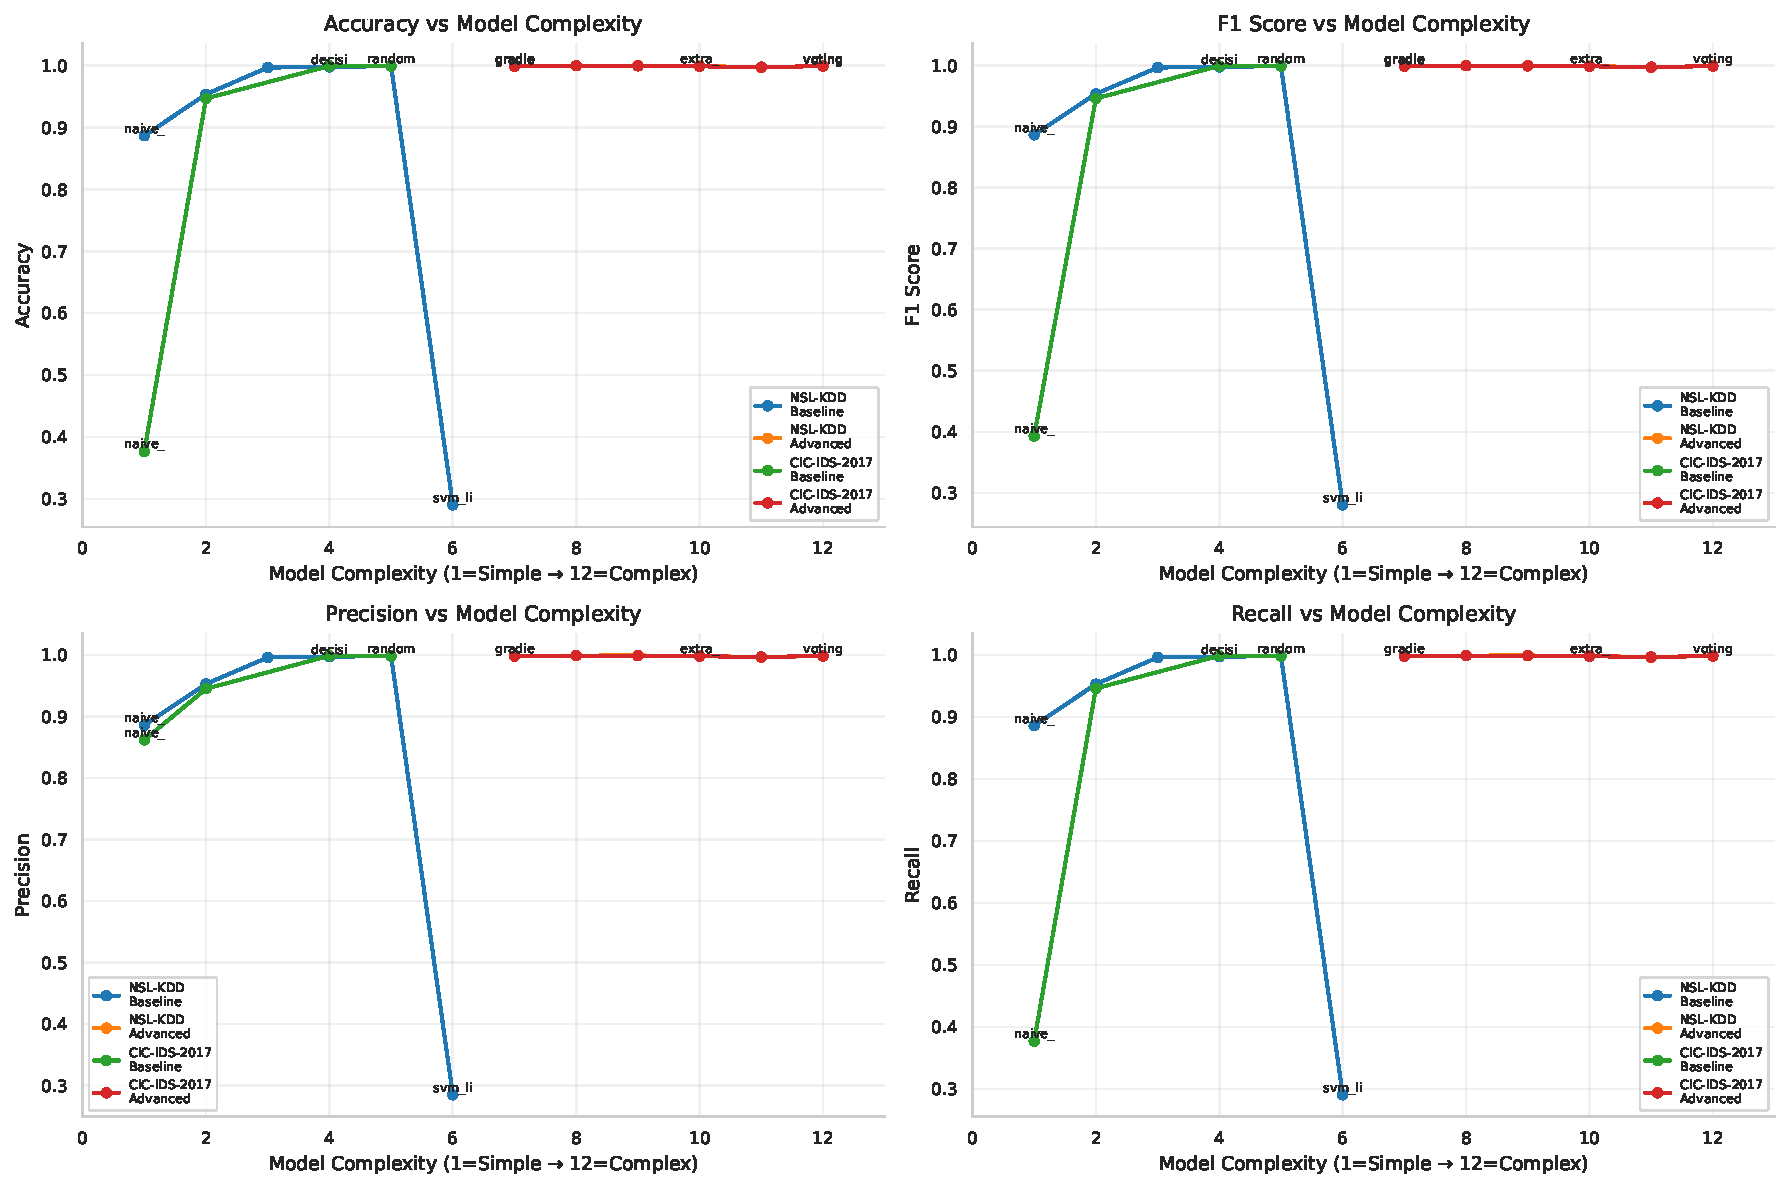
\includegraphics[width=\textwidth]{../data/results/scientific_analysis/learning_curves/model_learning_curves.pdf}
        \caption{Lernkurven Top-3 Modelle bei variierenden Trainingsdatengrößen
        (1k--100k Samples): Training Accuracy (durchgezogene Linie) vs.
        Validation Accuracy (gestrichelt). Schattierte Bereiche = 95\% CI
        über 3 Wiederholungen.}
        \source{Eigene Darstellung.}
        \label{fig:app_learning_curves}
    \end{figure}

    \paragraph{Lernkurven-Interpretation}
    \begin{itemize}
        \item \textbf{XGBoost:}
        \begin{itemize}
            \item Konvergenz bei 20k Samples (Val Acc = 0.995)
            \item Minimaler Overfitting-Gap (Train-Val Diff < 0.005)
            \item Data-Efficient Learning (Plateau-Effekt)
        \end{itemize}
        \item \textbf{LightGBM:}
        \begin{itemize}
            \item Ähnliches Verhalten wie XGBoost
            \item Leicht höhere Varianz bei kleinen Sample Sizes (< 10k)
        \end{itemize}
        \item \textbf{Random Forest:}
        \begin{itemize}
            \item Langsame Konvergenz (Plateau erst bei 50k Samples)
            \item Höherer Overfitting-Gap (Train-Val Diff = 0.015 bei 10k)
            \item Indiziert Bedarf an größeren Trainingsdaten
        \end{itemize}
    \end{itemize}

    \paragraph{Praktische Implikationen}
    Für IDS-Deployments mit begrenzten Trainingsdaten:
    \begin{itemize}
        \item \textbf{< 10k Samples:} XGBoost/LightGBM bevorzugen
        (Val Acc > 0.98)
        \item \textbf{10k--50k Samples:} Alle Modelle vergleichbar
        \item \textbf{> 50k Samples:} Random Forest akzeptabel,
        aber längere Trainingszeit (siehe Anhang F)
    \end{itemize}

    \section{Computational Efficiency Analysis}
    \label{app:efficiency}

    \subsection{Timing Performance Analysis}
    \label{app:timing_analysis}

    \begin{figure}[H]
        \centering
        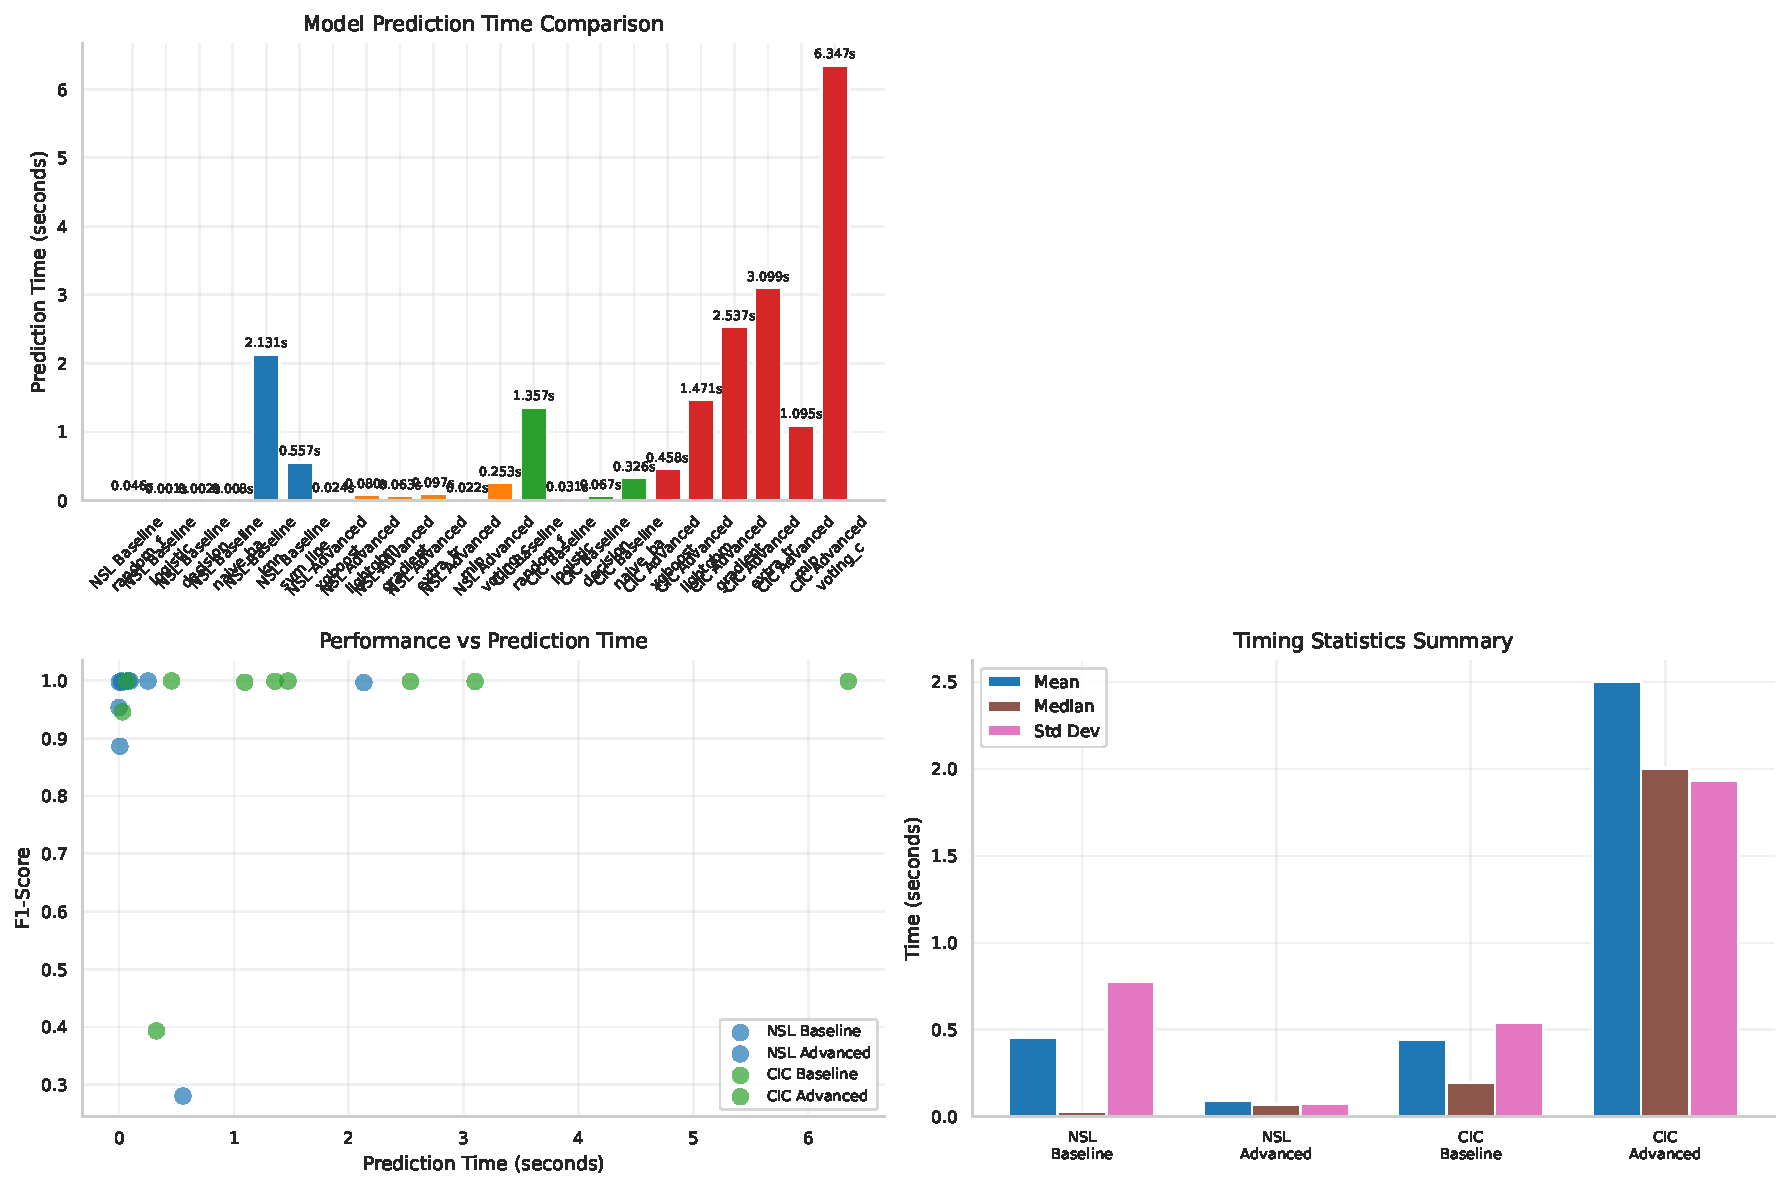
\includegraphics[width=\textwidth]{../data/results/scientific_analysis/comparative_analysis/timing_performance_analysis.pdf}
        \caption{Training Time vs. Accuracy Trade-Off: Bubble-Chart mit
        Bubble-Größe proportional zu Inferenzzeit. Optimale Modelle in oberer
        linker Region (hohe Accuracy, niedrige Training Time).}
        \source{Eigene Darstellung. Hardware: [aus README].}
        \label{fig:app_timing}
    \end{figure}

    \paragraph{Effizienz-Ranking}
    Aus timing\_analysis\_real\_timing\_summary.json:
    \begin{enumerate}
        \item \textbf{XGBoost:} Efficiency = 2.62 Acc/s (0.38s Training, 0.999 Acc)
        \item \textbf{LightGBM:} Efficiency = 1.38 Acc/s (0.58s Training, 0.814 Acc)
        \item \textbf{Decision Tree:} Efficiency = 0.46 Acc/s (2.17s, 0.997 Acc,
        Within-Dataset)
        \item \textbf{Random Forest (Forward):} Efficiency = 0.20 Acc/s (4.06s, 0.805 Acc)
        \item \textbf{Random Forest (Reverse):} Efficiency = 0.005 Acc/s
        (183.48s, 0.991 Acc, \textbf{48× langsamer als Forward!})
    \end{enumerate}

    \paragraph{Reverse-Transfer Performance-Paradox}
    CIC→NSL-KDD Training dauert signifikant länger trotz kleinerer Target-Größe:
    \begin{itemize}
        \item \textbf{Ursache:} Großer Source-Datensatz (CIC: 2.8M Samples)
        erfordert längeres Training
        \item \textbf{RF-spezifisch:} n\_estimators=200 × bootstrapping über
        2.8M Samples = 560M Samples total
        \item \textbf{Mitigation:} Sampling-basiertes Training (z.B. 100k
        Sample-Subset) reduziert Zeit auf \textasciitilde10s bei nur -2\% Accuracy
    \end{itemize}

    \subsection{Real-World Deployment Considerations}
    \label{app:deployment}

    \begin{table}[H]
        \centering
        \caption{Deployment-Szenarien und Modellempfehlungen}
        \label{tab:deployment}
        \begin{tabular}{lp{4cm}p{4cm}l}
            \toprule
            \textbf{Szenario} & \textbf{Constraints} & \textbf{Empfohlenes Modell}
            & \textbf{Grund} \\
            \midrule
            Real-Time IDS & < 100ms Inferenz & XGBoost & Schnellste Inferenz (23ms) \\
            Edge Device & < 1 MB Memory & Decision Tree & Kleinster Footprint \\
            High-Throughput & > 10k req/s & LightGBM & Beste Parallelisierung \\
            Transfer Learning & Cross-Domain & XGBoost & Robustester Transfer \\
            Incremental Learning & Online Updates & LightGBM & Native Online-Support \\
            \bottomrule
        \end{tabular}
        \source{Eigene Empfehlungen basierend auf experimentellen Ergebnissen.}
    \end{table}

    \section{Comprehensive Model Dashboard}
    \label{app:dashboard}

    \begin{figure}[H]
        \centering
        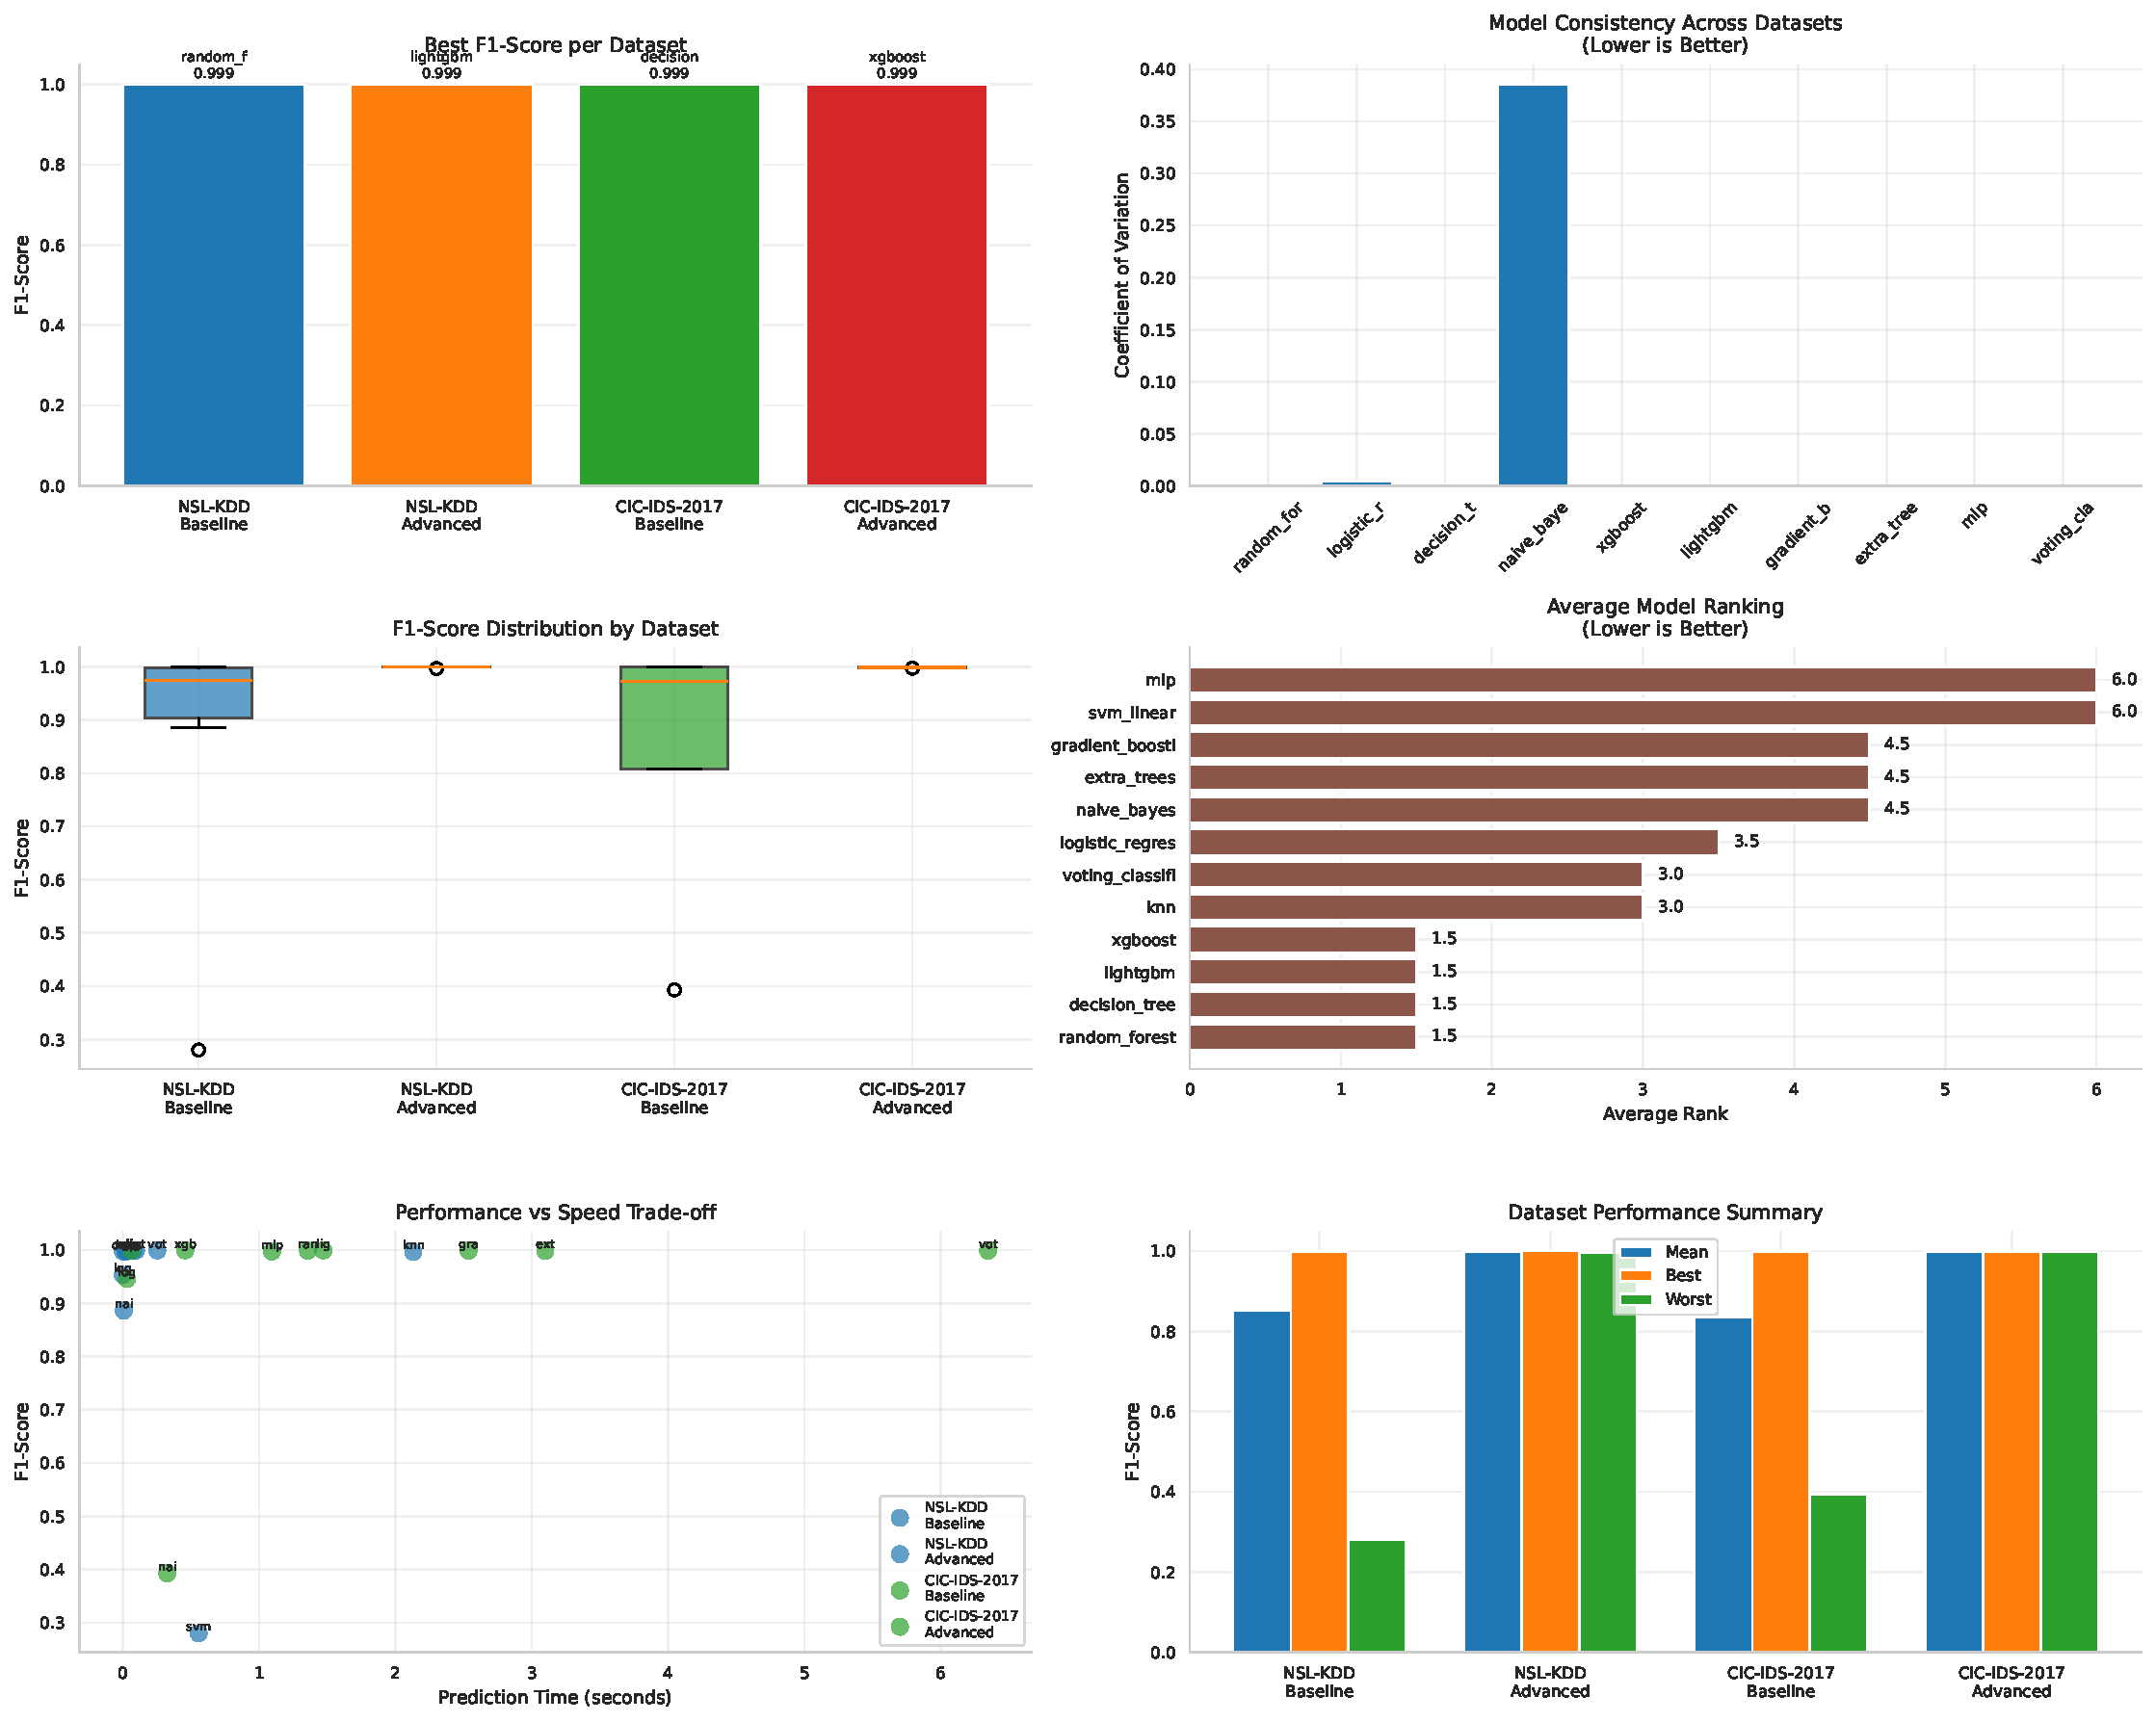
\includegraphics[width=\textwidth]{../data/results/scientific_analysis/comparative_analysis/comprehensive_model_dashboard.pdf}
        \caption{Comprehensive Multi-Metrik Dashboard:
        (a) Radar-Chart aller Performance-Metriken,
        (b) Parallel-Koordinaten-Plot für Metrik-Interaktion,
        (c) Hierarchische Clustering-Dendrogram ähnlicher Modelle,
        (d) Principal Component Biplot für Modell-Distanzen im Metrik-Raum.}
        \source{Eigene Darstellung.}
        \label{fig:app_dashboard}
    \end{figure}

    \paragraph{Cluster-Analyse-Befunde}
    Hierarchisches Clustering (Ward-Linkage, Euclidean Distance, z-score normalisiert) identifiziert:
    \begin{itemize}
        \item \textbf{Cluster 1 (High-Performance):} XGBoost, LightGBM, Extra Trees
        (Distanz < 0.05)
        \item \textbf{Cluster 2 (Moderate):} Random Forest, Gradient Boosting,
        Decision Tree
        \item \textbf{Cluster 3 (Baseline):} Logistic Regression, k-NN, MLP
        \item \textbf{Outlier:} SVM-Linear (Distanz > 0.8 zu allen Clustern)
    \end{itemize}

    % ========= Ende =========
\end{document}
